\section{eplusout.eio}\label{eplusout.eio}

This file contains some standard and some optional ``reports''. It is intended to be a somewhat intelligent report of input conditions when they don't fit well in other places or when they aren't substantial enough for their own ``file''. (e.g. \textbf{eplusout.bnd})~ Contents of the file are somewhat documented in various places in the \textbf{Input Output Reference document} -- as results of objects. This file or portions of it can be easily imported into spreadsheet programs and more analysis done there. Contents of this file include construction details, location information, site water mains temperature information, ``environment'' information, number of ``warmup'' days required in each environment.

The form of the file is a data dictionary line followed by the data. In this case, the data dictionary line precedes the first ``data'' line though there may be several defining ``dictionary lines''. Each dictionary line will show the field as \textless{}field name\textgreater{} followed by other fields that will be in the data lines. Data will be displayed similarly. Each field of dictionary or data will be separated from the next by a comma ``,'' -- and produce a comma delimited file. However, the lines for data will not be contiguous -- some follow a stream of consciousness of the EnergyPlus execution.

This section is subdivided into grouped sections by type.

Note that the lines in the eplusout.eio file can be extremely long (current limit is 500 characters).

\subsection{Simulation Parameters}\label{simulation-parameters}

! \textless{}Version\textgreater{}, Version ID

~Version, \textless{}version\textgreater{}

! \textless{}Timesteps per Hour\textgreater{}, \#TimeSteps, Minutes per TimeStep

~Timesteps Per Hour,~ 4, 15

! \textless{}Run Control\textgreater{}, Do Zone Sizing, Do System Sizing, Do Plant Sizing, Do Design Days, Do Weather Simulation

~Run Control, Yes, Yes, No, No, Yes

! \textless{}GroundTemperatures\textgreater{}, Months From Jan to Dec \{Deg C\}

~GroundTemperatures,~ 20.03,~ 20.03,~ 20.13,~ 20.30,~ 20.43,~ 20.52,~ 20.62,~ 20.77,~ 20.78,~ 20.55,~ 20.44,~ 20.20

! \textless{}GroundTemperatures:Surface\textgreater{}, Months From Jan to Dec \{Deg C\}

~GroundTemperatures:Surface,~ 18.00,~ 18.00,~ 18.00,~ 18.00,~ 18.00,~ 18.00,~ 18.00,~ 18.00,~ 18.00,~ 18.00,~ 18.00,~ 18.00

! \textless{}GroundTemperatures:Deep\textgreater{}, Months From Jan to Dec \{Deg C\}

~GroundTemperatures:Deep,~ 16.00,~ 16.00,~ 16.00,~ 16.00,~ 16.00,~ 16.00,~ 16.00,~ 16.00,~ 16.00,~ 16.00,~ 16.00,~ 16.00

! \textless{}GroundReflectances\textgreater{}, Months From Jan to Dec \{dimensionless\}

~GroundReflectances,~ 0.20,~ 0.20,~ 0.20,~ 0.20,~ 0.20,~ 0.20,~ 0.20,~ 0.20,~ 0.20,~ 0.20,~ 0.20,~ 0.20

! \textless{}Snow Ground Reflectance Modifiers\textgreater{}, Normal, Daylighting \{dimensionless\}

~Snow Ground Reflectance Modifiers,~~ 1.000,~~ 1.000

! \textless{}Snow GroundReflectances\textgreater{}, Months From Jan to Dec \{dimensionless\}

~Snow GroundReflectances,~ 0.20,~ 0.20,~ 0.20,~ 0.20,~ 0.20,~ 0.20,~ 0.20,~ 0.20,~ 0.20,~ 0.20,~ 0.20,~ 0.20

! \textless{}Snow GroundReflectances For Daylighting\textgreater{}, Months From Jan to Dec \{dimensionless\}

~Snow GroundReflectances For Daylighting,~ 0.20,~ 0.20,~ 0.20,~ 0.20,~ 0.20,~ 0.20,~ 0.20,~ 0.20,~ 0.20,~ 0.20,~ 0.20,~ 0.20

! \textless{}Location\textgreater{}, Location Name, Latitude \{N+/S- Deg\}, Longitude \{E+/W- Deg\},~ Time Zone Number \{GMT+/-\}, Elevation \{m\},~ Standard Pressure at Elevation \{Pa\}

Location,CHICAGO IL USA TMY2-94846 WMO\# = 725300,41.78,-87.75,-6.00,190.00,99063.

! \textless{}Site Water Mains Temperature Information\textgreater{}, Calculation Method\{\}, Water Mains Temperature Schedule Name\{\}, Annual Average Outdoor Air Temperature\{C\}, Maximum Difference In Monthly Average Outdoor Air Temperatures\{deltaC\}

~Site Water Mains Temperature Information, ,CorrelationFromWeatherFile,~ 9.99,~ 28.78

! \textless{}Building Information\textgreater{}, Building Name,North Axis \{deg\},Terrain,~ Loads Convergence Tolerance Value,Temperature Convergence Tolerance Value,~ Solar Distribution,Maximum Number of Warmup Days,Minimum Number of Warmup Days

~Building, BUILDING,~ 30.000,City,~~ 0.04000,~~ 0.40000,FullExterior,25,6

! Inside Convection Algorithm, Value \{Simple \textbar{} Detailed \textbar{} CeilingDiffuser\}

Inside Convection Algorithm,Simple

! Outside Convection Algorithm, Value \{Simple \textbar{} Detailed\}

Outside Convection Algorithm,Simple

! Solution Algorithm, Value \{CTF \textbar{} EMPD \textbar{} CONDFD \textbar{} HAMT\}

Solution Algorithm, CTF

! Sky Radiance Distribution, Value \{Anisotropic\}

Sky Radiance Distribution,Anisotropic

! \textless{}Environment:Site Atmospheric Variation\textgreater{},Wind Speed Profile Exponent \{\},Wind Speed Profile Boundary Layer Thickness \{m\},Air Temperature Gradient Coefficient \{K/m\}

Environment:Site Atmospheric Variation,0.330,460.000,6.500000E-003

! \textless{} Input Surface Geometry Information\textgreater{},Starting Corner,Vertex Input Direction,Coordinate System

~SurfaceGeometry,UpperLeftCorner,CounterClockwise,RelativeCoordinateSystem

The simulation parameters output is the simplest form of reporting in the \textbf{eplusout.eio} file. Each of the ``header'' records (lines starting with an ``!'') are followed immediately by the one and only data line. By and large, these data lines are all merely echoes of the entries in the IDF (or defaulted for blank fields). For most of these descriptions, you can look at the object fields (of same name) in the \href{file:///E:/Docs4PDFs/InputOutputReference.pdf}{Input Output Reference} document.

\subsection{Version}\label{version}

! \textless{}Version\textgreater{}, Version ID

~Version, \textless{}version\textgreater{}

This is the version of the IDF as entered in the IDF file. If it does not match the current EnergyPlus Version, a warning will be issued and show in the \textbf{eplusout.err} file.

\subsection{Timestep}\label{timestep}

! \textless{}Timesteps per Hour\textgreater{}, \#TimeSteps, Minutes per TimeStep

~Timesteps Per Hour,~ 4, 15

This is the number of timesteps in hour as entered in the IDF file as well as showing how many minutes will encompass each timestep (i.e.~4 timesteps in hour = 15 minutes per timestep).

\subsection{SimulationControl}\label{simulationcontrol}

! \textless{}Run Control\textgreater{}, Do Zone Sizing, Do System Sizing, Do Plant Sizing, Do Design Days, Do Weather Simulation, Do HVAC Sizing Simulation

~Run Control, Yes, Yes, Yes, No, Yes, No

This shows how the sizing and running (design days vs.~weather file) will be accomplished. Design days are required for sizing but do not necessarily need to be ``run'' after sizing has completed. Thus, the user can choose to do sizing, not do a ``normal'' calculation with the design day definitions but then go ahead and run the full simulation year. Some advanced sizing methods require also running HVAC Sizing Simulations.

\subsection{Building}\label{building}

! \textless{}Building Information\textgreater{}, Building Name,North Axis \{deg\},Terrain,~ Loads Convergence Tolerance Value,Temperature Convergence Tolerance Value,~ Solar Distribution,Maximum Number of Warmup Days

~Building Information, BUILDING,~ 30.000,City,~~ 0.04000,~~ 0.40000,FullExterior,25

This shows the values put in for the Building Object in the IDF.

\subsection{Inside Convection Algorithm}\label{inside-convection-algorithm}

! \textless{}Inside Convection Algorithm\textgreater{}, Value \{Simple \textbar{} Detailed \textbar{} CeilingDiffuser\}

Inside Convection Algorithm,Simple

This shows the global inside (interior) convection algorithm selected by the IDF value. This may be overridden by zone entries or even surface entries.

\subsection{Outside Convection Algorithm}\label{outside-convection-algorithm}

! \textless{}Outside Convection Algorithm\textgreater{}, Value \{Simple \textbar{} Detailed ! TARP ! MoWitt ! DOE-2 ! BLAST\}

Outside Convection Algorithm,Simple

This shows the global outside (exterior) convection algorithm selected by the IDF value. This may be overridden by zone entries or even surface entries.

\subsection{Solution Algorithm}\label{solution-algorithm}

! \textless{}Solution Algorithm\textgreater{}, Value \{CTF \textbar{} EMPD \textbar{} CONDFD \textbar{} HAMT\},Inside Surface Max Temperature Limit\{C\}

Solution Algorithm, CTF,200

This shows the solution algorithm approach selected by the IDF value and Inside Surface Max Temperature override or default value.

\subsection{Sky Radiance Distribution}\label{sky-radiance-distribution}

! \textless{}Sky Radiance Distribution\textgreater{}, Value \{Anisotropic\}

Sky Radiance Distribution,Anisotropic

This shows the solution algorithm approach used in the simulation. As this value cannot be changed by the user, it is shown for information only.

\subsection{Site Atmospheric Variation}\label{site-atmospheric-variation}

! \textless{}Environment:Site Atmospheric Variation\textgreater{},Wind Speed Profile Exponent \{\},Wind Speed Profile Boundary Layer Thickness \{m\},Air Temperature Gradient Coefficient \{K/m\}

Environment:Site Atmospheric Variation,0.330,460.000,6.500000E-003

This shows actual values used for Site Atmospheric Variations.

\subsection{Shadowing/Sun Position Calculations}\label{shadowingsun-position-calculations}

! \textless{}Shadowing/Sun Position Calculations\textgreater{} {[}Annual Simulations{]}, Calculation Method, Value \{days\}, Allowable Number Figures in Shadow Overlap \{\}, Polygon Clipping Algorithm, Sky Diffuse Modeling Algorithm

Shadowing/Sun Position Calculations, AverageOverDaysInFrequency, 20, 15000, SutherlandHodgman, SimpleSkyDiffuseModeling

This shows how many days between the re-calculation of solar position during a weather file simulation. While a smaller number of days will lead to a more accurate solar position estimation (solar position is important in shadowing as well as determining how much solar enters the space), it also increases the calculation time necessarily to complete the simulation. The default, re-calculating every 20 days, gives a good compromise. The allowable number of figures in a shadow overlap can be increased if necessary for the model. There are two calculation methods available: AverageOverDaysInFrequency (default) and DetailedTimestepIntegration.

\subsection{AirflowNetwork Model:Control}\label{airflownetwork-modelcontrol}

! \textless{}AirflowNetwork Model:Control\textgreater{}, No Multizone or Distribution/Multizone with Distribution/Multizone without Distribution/Multizone with Distribution only during Fan Operation

AirflowNetwork Model:Control,MultizoneWithoutDistribution

This shows the AirflowNetwork Model:Control selected by the IDF value in the object AirflowNetwork:SimulationControl.

\subsection{AirflowNetwork Model:Wind Direction}\label{airflownetwork-modelwind-direction}

! \textless{}AirflowNetwork Model:Wind Direction\textgreater{}, Wind Direction \#1 to n (degree)

AirflowNetwork Model:Wind Direction, 0.0,30.0,60.0,90.0,120.0,150.0,180.0,210.0,240.0,270.0,300.0,330.0

\subsubsection{Field: \textless{}AirflowNetwork Model:Wind Direction\textgreater{}}\label{field-airflownetwork-modelwind-direction}

This field contains the field name ``AirflowNetwork Model:Wind Direction''.

\subsubsection{Field: Wind Direction \#1 to n}\label{field-wind-direction-1-to-n}

These values are the wind directions corresponding to the first through the Nth wind pressure coefficient value. If Wind Pressure Coefficient Type = Input in the AirflowNetwork:SimulationControl object, the wind directions described here are the inputs specified in the AirflowNetwork:MultiZone:WindPressureCoefficientArray object,. If Wind Pressure Coefficient Type = SurfaceAverageCalculation in the AirflowNetwork:SimulationControl object, the wind directions are also described here and are fixed at 30 degree increments.

\subsection{AirflowNetwork Model:Wind Pressure Coefficients}\label{airflownetwork-modelwind-pressure-coefficients}

! \textless{}AirflowNetwork Model:Wind Pressure Coefficients\textgreater{}, Name, Wind Pressure Coefficients \#1 to n (dimensionless)

AirflowNetwork Model:Wind Pressure Coefficients, NFACADE\_WPCVALUE, 0.60,0.48,4.00E-002,-0.56,-0.56,-0.42,-0.37,-0.42,-0.56,-0.56,4.00E-002,0.48

AirflowNetwork Model:Wind Pressure Coefficients, EFACADE\_WPCVALUE, -0.56,4.00E-002,0.48,0.60,0.48,4.00E-002,-0.56,-0.56,-0.42,-0.37,-0.42,-0.56

AirflowNetwork Model:Wind Pressure Coefficients, SFACADE\_WPCVALUE, -0.37,-0.42,-0.56,-0.56,4.00E-002,0.48,0.60,0.48,4.00E-002,-0.56,-0.56,-0.42

AirflowNetwork Model:Wind Pressure Coefficients, WFACADE\_WPCVALUE, -0.56,-0.56,-0.42,-0.37,-0.42,-0.56,-0.56,4.00E-002,0.48,0.60,0.48,4.00E-002

\subsubsection{Field:~ \textless{} AirflowNetwork Model: Wind Pressure Coefficients\textgreater{}}\label{field-airflownetwork-model-wind-pressure-coefficients}

This field contains the constant ``AirflowNetwork Model: Wind Pressure Coefficients'' for each line.

\subsubsection{Field: Name}\label{field-name}

This is the WindPressureCoefficientValues object name entered from the IDF.

\subsubsection{Field: Wind Pressure Coefficients \#1 to n}\label{field-wind-pressure-coefficients-1-to-n}

These values are the wind pressure coefficient for the building façade. These wind pressure coefficient values correspond to the first through Nth wind directions reported above for \textless{}AirflowNetwork Model:Wind Direction\textgreater{}. If Wind Pressure Coefficient Type = INPUT in the AirflowNetwork:SimulationControl object, the wind pressure coefficients described here are the inputs specified in the AirflowNetwork:MultiZone:Wind Pressure Coefficient Values object,. If Wind Pressure Coefficient Type = SurfaceAverageCalculation in the AirflowNetwork:SimulationControl object, the wind pressure coefficients are calculated internally and also described here.

\subsection{Zone Volume Capacitance Multiplier}\label{zone-volume-capacitance-multiplier}

! \textless{}Zone Volume Capacitance Multiplier\textgreater{}, Sensible Heat Capacity Multiplier, Moisture Capacity Multiplier, Carbon Dioxide Capacity Multiplier, Generic Contaminant Capacity Multiplier

Zone Volume Capacitance Multiplier,~~ 1.000, 1.000, 1.000, 1.000

This shows the zone volume capacitance multipliers selected by the IDF value or defaulted. The object for this item is ZoneCapacitanceMultiplier:ResearchSpecial.

\subsubsection{Field: Sensible Heat Capacity Multiplier}\label{field-sensible-heat-capacity-multiplier}

Value used to alter the effective heat capacitance of the zone air volume.

\subsubsection{Field: Moisture Capacity Multiplier}\label{field-moisture-capacity-multiplier}

Value used to alter the effective moisture capacitance of the zone air volume.

\subsubsection{Field: Carbon Dioxide Capacity Multiplier}\label{field-carbon-dioxide-capacity-multiplier}

Value used to alter the effective carbon dioxide capacitance of the zone air volume.

\subsubsection{Field: Generic Contaminant Capacity Multiplier}\label{field-generic-contaminant-capacity-multiplier}

Value used to alter the effective generic contaminant capacitance of the zone air volume.

\subsubsection{Surface Geometry}\label{surface-geometry}

! \textless{}SurfaceGeometry\textgreater{},Starting Corner,Vertex Input Direction,Coordinate System,Daylight Reference Point Coordinate System,Rectangular (Simple) Surface Coordinate System

Surface Geometry, UpperLeftCorner, Counterclockwise, RelativeCoordinateSystem, RelativeCoordinateSystem, RelativeToZoneOrigin

This shows the expected order of the vertices for each surface. The object for this item is GlobalGeometryRules.

\subsubsection{Field: Starting Corner}\label{field-starting-corner}

Value used to designate which corner the surface(s) start with.

\subsubsection{Field: Vertex Input Direction}\label{field-vertex-input-direction}

Value whether the coordinates for the surface are entered clockwise or counter-clockwise.

\subsubsection{Field: Coordinate System}\label{field-coordinate-system}

Value whether the coordinate system is World/Absolute or Relative.

\subsubsection{Field: Daylight Reference Point Coordinate System}\label{field-daylight-reference-point-coordinate-system}

If daylighting is used, this describes the coordinate system for entering daylight reference points.

\subsubsection{Field: Rectangular (Simple) Surface Coordinate System}\label{field-rectangular-simple-surface-coordinate-system}

For simple surfaces (Wall, Window, Door, and so forth) the coordinate system that is used to describe their starting point.

\subsubsection{Field: Number Nominal Surfaces}\label{field-number-nominal-surfaces}

This is the number of ``nominal'' surfaces (based on surface objects) that a quick calculation from the program has found. If the number of surfaces is not greater than 30, then the number of threads to be used will be set by the program to 1.

\subsubsection{Field: Number Parallel Sims}\label{field-number-parallel-sims}

This is the number of windowed/parallel simulations being run simultaneously as set by EP-Launch or other scripts distributed with the EnergyPlus program. Third party distributions may also set this item.

\subsection{Climate Group Outputs}\label{climate-group-outputs}

Climate related variables appear in two places for EnergyPlus outputs. Certain objects that are invariant throughout a simulation period have lines appear in the eplusout.eio file:

! \textless{}Environment:Weather Station\textgreater{},Wind Sensor Height Above Ground \{m\},Wind Speed Profile Exponent \{\},Wind Speed Profile Boundary Layer Thickness \{m\},Air Temperature Sensor Height Above Ground \{m\},Wind Speed Modifier Coefficient {[}Internal{]},Temperature Modifier Coefficient {[}Internal{]}

Environment:Weather Station,10.000,0.140,270.000,1.500,1.586,9.750E-003

! \textless{}Environment:Site Atmospheric Variation\textgreater{},Wind Speed Profile Exponent \{\},Wind Speed Profile Boundary Layer Thickness \{m\},Air Temperature Gradient Coefficient \{K/m\}

Environment:Site Atmospheric Variation,~~ 0.220, 370.000, 0.006500

! \textless{}Location\textgreater{}, Location Name, Latitude, Longitude, Time Zone Number, Elevation \{m\}

~Location, DENVER COLORADO,~~ 39.75, -104.87,~~ -7.00,~~~~~ 1610.26

! \textless{}Site Water Mains Temperature Information\textgreater{}, Calculation Method\{\}, Water Mains Temperature Schedule Name\{\}, Annual Average Outdoor Air Temperature\{C\}, Maximum Difference In Monthly Average Outdoor Air Temperatures\{deltaC\}

~Site Water Mains Temperature Information, ,~CorrelationFromWeatherFile,~ 9.99,~ 28.78

In addition for each ``environment'' simulated, information about the environment is shown:

! \textless{}Environment\textgreater{},Environment Name,Environment Type, Start Date, End Date, Start DayOfWeek, Duration \{\#days\}, Source:Start DayOfWeek,~ Use Daylight Savings, Use Holidays, Apply Weekend Holiday Rule

! \textless{}Environment:Special Days\textgreater{}, Special Day Name, Special Day Type, Source, Start Date, Duration \{\#days\}

! \textless{}Environment:Daylight Saving\textgreater{}, Daylight Saving Indicator, Source, Start Date, End Date

! \textless{}Environment:Design\_Day\_Misc\textgreater{},DayOfYear,ASHRAE A Coeff,ASHRAE B Coeff,ASHRAE C Coeff,Solar Constant-Annual Variation,Eq of Time \{minutes\}, Solar Declination Angle \{deg\}, Solar Model

! \textless{}Environment:WarmupDays\textgreater{}, NumberofWarmupDays

For example, a DesignDay:

Environment,PHOENIX ARIZONA WINTER,DesignDay, 1/21, 1/21,MONDAY,~ 1,N/A,N/A,N/A,N/A

Environment:Daylight Saving,No,DesignDay

Environment:Design\_Day\_Misc, 21,1228.9,0.1414,5.7310E-002,1.0,-11.14,-20.0

A Design RunPeriod:

Environment,EXTREME SUMMER WEATHER PERIOD FOR DESIGN,User Selected WeatherFile Typical/Extreme Period (Design) = Summer Extreme,07/13,07/19,SummerDesignDay,~ 7,Use RunPeriod Specified Day,No ,No ,No ,No ,No

Environment:Daylight Saving,No,RunPeriod Object

Environment:WarmupDays,~ 3

Or a RunPeriod (Name listed in the RunPeriod output is dependent on user input for the RunPeriod object -- when a blank is input, the name of the weather file location is used):

Environment,CHICAGO IL TMY2-94846 WMO\# = 725300,WeatherRunPeriod, 1/ 1,12/31,SUNDAY,365,UseWeatherFile,Yes,Yes,No

Environment:Daylight Saving,No,

Environment:Special Days,NEW YEARS DAY,Holiday,WeatherFile, 1/ 1,~ 1

Environment:Special Days,MEMORIAL DAY,Holiday,WeatherFile, 5/31,~ 1

Environment:Special Days,INDEPENDENCE DAY,Holiday,WeatherFile, 7/ 5,~ 1

Environment:Special Days,LABOR DAY,Holiday,WeatherFile, 9/ 6,~ 1

Environment:Special Days,THANKSGIVING,Holiday,WeatherFile,11/25,~ 1

Environment:Special Days,CHRISTMAS,Holiday,WeatherFile,12/25,~ 1

Environment:WarmupDays,~ 4

Note that in this display, using ``weekend rule'' and specific date holidays, the actual observed dates are shown in the output display -- in the example above, Independence Day (July 4) is actually observed on July 5.

\subsection{Climate Group -- Simple Outputs}\label{climate-group-simple-outputs}

Some of the climate outputs are a ``simple'' group. The ``header'' line is followed immediately by the data line.

\subsection{Location}\label{location}

This output represents the location data used for the simulation. Note that if a runperiod is used, the IDF ``Location'' is ignored and the location from the weather file is used instead.

\subsubsection{Field: \textless{}Location\textgreater{}}\label{field-location}

This data field will contain the constant ``Location''.

\subsubsection{Field: Location Name}\label{field-location-name}

This is the name given to the location whether from the IDF or the weather file.

\subsubsection{Field: Latitude}\label{field-latitude}

This is the latitude of the site, expressed decimally. Convention uses positive (+) values for North of the Equator and negative (-) values for South of the Equator. For example, S 30° 15' is expressed as --30.25.

\subsubsection{Field: Longitude}\label{field-longitude}

This is the longitude of the site, expressed decimally. Convention uses positive (+) values for East of the Greenwich meridian and negative (-) values for West of the Greenwich meridian. For example, E 130° 45' is expressed as +130.75.

\subsubsection{Field: Time Zone Number}\label{field-time-zone-number}

This is the time zone of the site, expressed decimally. Convention uses positive (+) values for GMT+ (Longitude East of the Greenwich meridian) and negative (-) values for GMT- (Longitude West of the Greenwich meridian). For example, the time zone for Central US time is --6. The time zone for parts of Newfoundland is --3.5 (-3 hours, 30 minutes from GMT).

\subsubsection{Field: Elevation \{m\}}\label{field-elevation-m}

This is the elevation of the site. Units are m.

\subsection{Site Water Mains Temperature}\label{site-water-mains-temperature}

This data field will contain the object ``Site:WaterMainsTemperature''.

\subsubsection{Calculation Method}\label{calculation-method}

This is calculation method used to determine site water mains temperature at each time step. Valid choices are: ``Schedule'', ``Correlation'' or ``CorrelationFromWeatherFile''.

\subsubsection{Water Mains Temperature Schedule Name}\label{water-mains-temperature-schedule-name}

This is name of a schedule that contains site water mains temperature for each time step.

\subsubsection{Annual Average Outdoor Air Temperature}\label{annual-average-outdoor-air-temperature}

This is the annual average outdoor air dry-bulb temperature for the site.

\subsubsection{Maximum Difference In Monthly Average Outdoor Air Temperatures}\label{maximum-difference-in-monthly-average-outdoor-air-temperatures}

This is the maximum difference in monthly-daily average of the outdoor air dry-bulb temperature for the site.

\subsection{Weather Station}\label{weather-station}

\subsubsection{Field: Wind Sensor Height Above Ground \{m\}}\label{field-wind-sensor-height-above-ground-m}

This is the wind sensor height above ground for weather data measurements.

\subsubsection{Field: Wind Speed Profile Exponent}\label{field-wind-speed-profile-exponent}

The wind speed profile exponent for the terrain surrounding the weather station.

\subsubsection{Field: Wind Speed Profile Boundary Layer Thickness \{m\}}\label{field-wind-speed-profile-boundary-layer-thickness-m}

The wind speed profile boundary layer thickness {[}m{]} for the terrain surrounding the weather station.

\subsubsection{Field: Air Temperature Sensor Height Above Ground \{m\}}\label{field-air-temperature-sensor-height-above-ground-m}

The height {[}m{]} above ground for the air temperature sensor.

\subsubsection{Field: Wind Speed Modifier Coefficient {[}Internal{]}}\label{field-wind-speed-modifier-coefficient-internal}

This field is intended to provide a slight help for the user to determine the calculations that will be used to calculate the Wind Speed at a specific height at the site.

The full calculation for Local Wind Speed is:

\begin{equation}
\text{LocalWindSpeed} = \text{WindSpeed}_{met} \left( \frac{\text{WindBoundaryLayerThickness}_{met}}{\text{AirSensorHeight}_{met}} \right)^{\text{WindExponent}_{met}} \left(\frac{\text{HeightAboveGround}_{site/component}}{\text{WindBoundaryLayerThickness}_{site}}\right)^{\text{SiteWindExponent}}
\end{equation}

The Wind Speed Modifier Coefficient {[}Internal{]} simplifies the equation to:

\begin{equation}
\text{LocalWindSpeed} = \text{WindSpeed}_{met} \left( \text{WindSpeedModifier} \right) \left(\frac{\text{HeightAboveGround}_{site/component}}{\text{WindBoundaryLayerThickness}_{site}}\right)^{\text{SiteWindExponent}}
\end{equation}

Where the Wind Speed Modifier encapsulates:

\begin{equation}
\text{WindSpeedModifier} = \left( \frac{\text{WindBoundaryLayerThickness}_{met}}{\text{AirSensorHeight}_{met}} \right)^{\text{WindExponent}_{met}}
\end{equation}

Where

\begin{itemize}
\tightlist
\item
  met = meteorological station
\item
  site = location of the building
\end{itemize}

\subsubsection{Field:Temperature Modifier Coefficient {[}Internal{]}}\label{fieldtemperature-modifier-coefficient-internal}

This field is intended to provide a slight help for the user to determine the calculations that will be used to calculate the air (dry-bulb) or wet-bulb temperature at a specific height at the site.

The site temperature modifier coefficient (TMC) is defined as:

\begin{equation}
TMC = frac{ \text{AtmosphericTemperatureGradient} \cdot \text{EarthRadius} \cdot \text{TemperatureSensorHeight}_{met} }
                  { \text{EarthRadius} + \text{TemperatureSensorHeight}_{met} }
\end{equation}

Then, the temperature at a height above ground is calculated as:

\begin{equation}
\text{ActualTemperature} = \text{Temperature}_{met} + TMC -
    frac{ \text{TemperatureGradient}_{site} * \text{EarthRadius} * \text{Height}_{site/component} }
        { \text{EarthRadius} + \text{Height}_{site/component} }
\end{equation}

Where

\begin{itemize}
\tightlist
\item
  met = meteorological station
\item
  site = location of the building
\end{itemize}

\subsection{Site Atmospheric Variation}\label{site-atmospheric-variation-1}

\subsubsection{Field: Wind Speed Profile Exponent}\label{field-wind-speed-profile-exponent-1}

The wind speed profile exponent for the terrain surrounding the site.

\subsubsection{Field: Wind Speed Profile Boundary Layer Thickness \{m\}}\label{field-wind-speed-profile-boundary-layer-thickness-m-1}

The wind speed profile boundary layer thickness {[}m{]} for the terrain surrounding the site.

\subsubsection{Field: Air Temperature Gradient Coefficient \{K/m\}}\label{field-air-temperature-gradient-coefficient-km}

The air temperature gradient coefficient {[}K/m{]} is a research option that allows the user to control the variation in outdoor air temperature as a function of height above ground. The real physical value is 0.0065 K/m.

\subsection{Ground Temperatures and Ground Reflectances}\label{ground-temperatures-and-ground-reflectances}

! \textless{}Site:GroundTemperature:BuildingSurface\textgreater{}, Months From Jan to Dec \{Deg C\}

~Site:GroundTemperature:BuildingSurface,~ 20.03,~ 20.03,~ 20.13,~ 20.30,~ 20.43,~ 20.52,~ 20.62,~ 20.77,~ 20.78,~ 20.55,~ 20.44,~ 20.20

! \textless{}Site:GroundTemperature:FCfactorMethod\textgreater{}, Months From Jan to Dec \{Deg C\}

~Site:GroundTemperature:FCfactorMethod,~ -1.89,~ -3.06,~ -0.99,~~ 2.23,~ 10.68,~ 17.20,~ 21.60,~ 22.94,~ 20.66,~ 15.60,~~ 8.83,~~ 2.56

! \textless{}Site:GroundTemperature:Shallow\textgreater{}, Months From Jan to Dec \{Deg C\}

~Site:GroundTemperature:Shallow,~ 13.00,~ 13.00,~ 13.00,~ 13.00,~ 13.00,~ 13.00,~ 13.00,~ 13.00,~ 13.00,~ 13.00,~ 13.00,~ 13.00

! \textless{}Site:GroundTemperature:Deep\textgreater{}, Months From Jan to Dec \{Deg C\}

~Site:GroundTemperature:Deep,~ 16.00,~ 16.00,~ 16.00,~ 16.00,~ 16.00,~ 16.00,~ 16.00,~ 16.00,~ 16.00,~ 16.00,~ 16.00,~ 16.00

! \textless{}Site:GroundReflectance\textgreater{}, Months From Jan to Dec \{dimensionless\}

~Site:GroundReflectance,~ 0.20,~ 0.20,~ 0.20,~ 0.20,~ 0.20,~ 0.20,~ 0.20,~ 0.20,~ 0.20,~ 0.20,~ 0.20,~ 0.20

! \textless{}Site:GroundReflectance:SnowModifier\textgreater{}, Normal, Daylighting \{dimensionless\}

~Site:GroundReflectance:SnowModifier,~~ 1.000,~~ 1.000

! \textless{}Site:GroundReflectance:Snow\textgreater{}, Months From Jan to Dec \{dimensionless\}

~Site:GroundReflectance:Snow,~ 0.20,~ 0.20,~ 0.20,~ 0.20,~ 0.20,~ 0.20,~ 0.20,~ 0.20,~ 0.20,~ 0.20,~ 0.20,~ 0.20

! \textless{}Site:GroundReflectance:Snow:Daylighting\textgreater{}, Months From Jan to Dec \{dimensionless\}

~Site:GroundReflectance:Snow:Daylighting,~ 0.20,~ 0.20,~ 0.20,~ 0.20,~ 0.20,~ 0.20,~ 0.20,~ 0.20,~ 0.20,~ 0.20,~ 0.20,~ 0.20

\subsection{Ground Temperatures}\label{ground-temperatures}

\subsubsection{Field: \textless{}GroundTemperatures\textgreater{}}\label{field-groundtemperatures}

This data field will contain the constant ``GroundTemperatures''.

\subsubsection{Field Set (1-12) -- Monthly Ground Temperatures}\label{field-set-1-12-monthly-ground-temperatures}

There will be a set of 12 numbers -- the ground temperatures by month: January, February, March, April, May, June, July, August, September, October, November, December. Units are C.

\subsection{Ground Reflectance}\label{ground-reflectance}

\subsubsection{Field: \textless{}GroundReflectances\textgreater{}}\label{field-groundreflectances}

This data field will contain the constant ``GroundReflectances''.

\subsubsection{Field Set (1-12) -- Monthly Ground Reflectances}\label{field-set-1-12-monthly-ground-reflectances}

There will be a set of 12 numbers -- the ground reflectances by month: January, February, March, April, May, June, July, August, September, October, November, December.

\subsection{Snow Ground Reflectance Modifiers}\label{snow-ground-reflectance-modifiers}

It is generally accepted that snow resident on the ground increases the basic ground reflectance. EnergyPlus allows the user control over the snow ground reflectance for both ``normal ground reflected solar'' calculations (see above) and snow ground reflected solar modified for daylighting. This is the display of the user entered or defaulted values.

\subsubsection{Field: \textless{}Snow Ground Reflectance~ Modifiers\textgreater{}}\label{field-snow-ground-reflectance-modifiers}

This data field will contain the constant ``Snow Ground Reflectance Modifiers''.

\subsubsection{Field: Normal}\label{field-normal}

This field is the value between 0.0 and 1.0 which is used to modified the basic monthly ground reflectance when snow is on the ground (from design day input or weather data values).

\begin{equation}
\text{GroundReflectance}_{used} = \text{GroundReflectance} \cdot \text{Modifier}_{snow}
\end{equation}

\subsubsection{Field: Daylighting}\label{field-daylighting}

This field is the value between 0.0 and 1.0 which is used to modified the basic monthly ground reflectance when snow is on the ground (from design day input or weather data values).

\begin{equation}
\text{DaylightingGroundReflectance}_{used} = \text{GroundReflectance} \cdot \text{Modifier}_{snow}
\end{equation}

\subsection{Snow Ground Reflectance}\label{snow-ground-reflectance}

This data is the result of using the Snow Ground Reflectance modifier and the basic Ground Reflectance value.

\subsubsection{Field: \textless{}GroundReflectances\textgreater{}}\label{field-groundreflectances-1}

This data field will contain the constant ``Snow GroundReflectances''.

\subsubsection{Field Set (1-12) -- Monthly Snow Ground Reflectances}\label{field-set-1-12-monthly-snow-ground-reflectances}

There will be a set of 12 numbers -- the snow ground reflectances by month: January, February, March, April, May, June, July, August, September, October, November, December.

\subsection{Snow Ground Reflectance for Daylighting}\label{snow-ground-reflectance-for-daylighting}

This data is the result of using the Snow Ground Reflectance for Daylighting modifier and the basic Ground Reflectance value.

\subsubsection{Field: \textless{} Snow GroundReflectances For Daylighting\textgreater{}}\label{field-snow-groundreflectances-for-daylighting}

This data field will contain the constant ``Snow GroundReflectances For Daylighting''.

\subsubsection{Field Set (1-12) -- Monthly Snow Ground Reflectances for Daylighting}\label{field-set-1-12-monthly-snow-ground-reflectances-for-daylighting}

There will be a set of 12 numbers -- the ground reflectances by month: January, February, March, April, May, June, July, August, September, October, November, December.

\subsection{Climate Group -- Not so Simple Outputs}\label{climate-group-not-so-simple-outputs}

For each ``environment'' simulated, a set of outputs is produced. The header group is only produced once. (The Design Day Misc header is produced only when there is a design day.)

! \textless{}Environment\textgreater{},Environment Name,Environment Type, Start Date, End Date, Start DayOfWeek, Duration \{\#days\}, Source:Start DayOfWeek,~ Use Daylight Saving, Use Holidays, Apply Weekend Holiday Rule

! \textless{}Environment:Special Days\textgreater{}, Special Day Name, Special Day Type, Source, Start Date, Duration \{\#days\}

! \textless{}Environment:Daylight Saving\textgreater{}, Daylight Saving Indicator, Source, Start Date, End Date

! \textless{}Environment:Design\_Day\_Misc\textgreater{},DayOfYear,ASHRAE A Coeff,ASHRAE B Coeff,ASHRAE C Coeff,Solar Constant-Annual Variation,Eq of Time \{minutes\}, Solar Declination Angle \{deg\}

! \textless{}Environment:WarmupDays\textgreater{}, NumberofWarmupDays

\subsection{Environment Line}\label{environment-line}

Each ``environment'' (i.e.~each design day, each run period) will have this line shown.

\subsubsection{Field: \textless{}Environment\textgreater{}}\label{field-environment}

This field will have the constant ``Environment'' in each data line.

\subsubsection{Field:Environment Name}\label{fieldenvironment-name}

This field will have the ``name'' of the environment. For example, the design day name (``DENVER COLORADO SUMMER'') or the weather file location name (``BOULDER CO TMY2-94018 WMO\# = 724699'').

\subsubsection{Field:Environment Type}\label{fieldenvironment-type}

This will be ``DesignDay'' for design day simulations and ``WeatherRunPeriod'' for weather file run periods.

\subsubsection{Field: Start Date}\label{field-start-date}

This will have the month/day that is the starting date for the simulation period. (7/21, for example).

\subsubsection{Field: End Date}\label{field-end-date}

This will have the month/day that is the ending date for the simulation period. Note that Design Days are only one day and the end date will be the same as the start date.

\subsubsection{Field: Start DayOfWeek}\label{field-start-dayofweek}

For weather periods, this will be the designated starting day of week. For design days, it will be the day type listed for the design day object (e.g.~SummerDesignDay or Monday).

\subsubsection{Field: Duration \{\#days\}}\label{field-duration-days}

Number of days in the simulation period will be displayed in this field. Design days are only 1 day.

\subsubsection{Field: Source:Start DayOfWeek}\label{field-sourcestart-dayofweek}

This field will list the ``source'' of the Start Day of Week listed earlier. This could be the RunPeriod command from the input file or the Weather File if the UseWeatherFile option was chosen in the RunPeriod command. For design days, this will be ``N/A''.

\subsubsection{Field: Use Daylight Saving}\label{field-use-daylight-saving}

This field reflects the value of the Use Daylight Saving field of the RunPeriod object. For design days, this will be ``N/A''.

\subsubsection{Field: Use Holidays}\label{field-use-holidays}

This field reflects the value of the Use Holidays field of the RunPeriod object. For design days, this will be ``N/A''.

\subsubsection{Field: Apply Weekend Holiday Rule}\label{field-apply-weekend-holiday-rule}

For design days, this will show ``N/A''. For weather periods, this will show ``Yes'' if the Apply Weekend Holiday Rule is in effect or ``No'' if it isn't.

\subsection{Design Day Misc Line}\label{design-day-misc-line}

This line is shown for each design day simulated. It is not shown for sizing runs that do not subsequently use the design day as a simulation period.

\subsubsection{Field: \textless{}Design Day Misc\textgreater{}}\label{field-design-day-misc}

This is a constant that will display ``Environment:Design\_Day\_Misc''.

\subsubsection{Field:DayOfYear}\label{fielddayofyear}

This is the Julian day of year for the design day (i.e.~Jan 1 is 1, Jan 31 is 31).

\subsubsection{Field:ASHRAE A Coeff}\label{fieldashrae-a-coeff}

Reference ASHRAE HOF 30 -- this is the A Coefficient in Wh/m\(^{2}\) calculated from EnergyPlus.

\subsubsection{Field:ASHRAE B Coeff}\label{fieldashrae-b-coeff}

Likewise, this is the ASHRAE B Coefficient (dimensionless).

\subsubsection{Field:ASHRAE C Coeff}\label{fieldashrae-c-coeff}

This is the ASHRAE C Coefficient (dimensionless).

\subsubsection{Field:Solar Constant-Annual Variation}\label{fieldsolar-constant-annual-variation}

This is the calculated solar constant using the given location and day of year.

\subsubsection{Field:Eq of Time \{minutes\}}\label{fieldeq-of-time-minutes}

This is the calculated equation of time (minutes) using the given location and day of year.

\subsubsection{Field: Solar Declination Angle \{deg\}}\label{field-solar-declination-angle-deg}

This is the solar declination angle for the day of year, degrees.

\subsection{Special Day Line}\label{special-day-line}

\subsubsection{Field: \textless{}Environment:Special Days\textgreater{}}\label{field-environmentspecial-days}

This is a constant that will display ``Environment:SpecialDays''.

\subsubsection{Field: Special Day Name}\label{field-special-day-name}

This is the user designated name for the special day.

\subsubsection{Field: Special Day Type}\label{field-special-day-type}

This shows the type for the special day (e.g.~Holiday).

\subsubsection{Field: Source}\label{field-source}

This will display ``InputFile'' if it was specified in the IDF or ``WeatherFile'' if it came from the weather file designation.

\subsubsection{Field: Start Date}\label{field-start-date-1}

This shows the starting date as month/day (e.g.~7/4).

\subsubsection{Field: Duration \{\#days\}}\label{field-duration-days-1}

This shows how many days the special day period continues. Usually, holidays are only 1 day duration.

\subsection{Daylight Saving Line}\label{daylight-saving-line}

\subsubsection{Field: \textless{}Environment:Daylight Saving\textgreater{}}\label{field-environmentdaylight-saving}

This is a constant that will display ``Environment:DaylightSaving''.

\subsubsection{Field: Daylight Saving Indicator}\label{field-daylight-saving-indicator}

This will be Yes if daylight saving is to be observed for this simulation period and No if it is not observed.

\subsubsection{Field: Source}\label{field-source-1}

This will show the source of this invocation (or non-invocation). Inputfile if DaylightSavingPeriod was entered (weather files only), WeatherFile if used in the Weather file and selected in the Run Period object and designday if that was the source.

\subsubsection{Field: Start Date}\label{field-start-date-2}

If the indicator field is Yes, then this field will be displayed and the month/day (e.g.~4/1) that starts the daylight saving period observance will be shown.

\subsubsection{Field: End Date}\label{field-end-date-1}

If the indicator field is Yes, then this field will be displayed and the month/day (e.g.~10/29) that ends the daylight saving period observance will be shown.

\subsection{Zone Outputs}\label{zone-outputs}

\subsection{Zone Summary}\label{zone-summary}

An overall zone summary is shown:

! \textless{}Zone Summary\textgreater{}, Number of Zones, Number of Surfaces, Number of SubSurfaces

~Zone Summary,19,158,12

As indicated:

\subsubsection{Field: \textless{}Zone Summary\textgreater{}}\label{field-zone-summary}

This field contains the constant ``Zone Summary''.

\subsubsection{Field: Number of Zones}\label{field-number-of-zones}

This field will contain the number of zones in the simulation.

\subsubsection{Field: Number of Surfaces}\label{field-number-of-surfaces}

This field will contain the total number of surfaces in the simulation.

\subsubsection{Field: Number of SubSurfaces}\label{field-number-of-subsurfaces}

This field will contain the total number of subsurfaces in the simulation.

\subsection{Zone Information}\label{zone-information}

Each zone is summarized in a simple set of statements as shown below:

! \textless{}Zone Information\textgreater{},Zone Name,North Axis \{deg\},Origin X-Coordinate \{m\},Origin Y-Coordinate \{m\},Origin Z-Coordinate \{m\},Centroid X-Coordinate \{m\},Centroid Y-Coordinate \{m\},Centroid Z-Coordinate \{m\},Type,Zone Multiplier,Zone List Multiplier,Minimum X \{m\},Maximum X \{m\},Minimum Y \{m\},Maximum Y \{m\},Minimum Z \{m\},Maximum Z \{m\},Ceiling Height \{m\},Volume \{m3\},Zone Inside Convection Algorithm \{Simple-Detailed-CeilingDiffuser-TrombeWall\},Zone Outside Convection Algorithm \{Simple-Detailed-Tarp-MoWitt-DOE-2-BLAST\}, Floor Area \{m2\},Exterior Gross Wall Area \{m2\},Exterior Net Wall Area \{m2\},Exterior Window Area \{m2\}, Number of Surfaces, Number of SubSurfaces, Number of Shading SubSurfaces,~ Part of Total Building Area

~Zone Information, PSI FOYER,0.0,0.00,0.00,0.00,8.56,-1.80,2.27,1,1,1,0.00,16.34,-9.51,4.88,0.00,6.10,3.81,368.12,Detailed,DOE-2,96.62,70.61,70.61,106.84,6,1,0,Yes

~Zone Information, DORM ROOMS AND COMMON AREAS,0.0,0.00,6.10,0.00,18.35,11.26,3.05,1,1,1,3.57,31.70,-4.75,25.36,0.00,6.10,6.10,2723.33,Detailed,DOE-2,445.93,312.15,267.56,52.59,10,22,0,Yes

~Zone Information, LEFT FORK,-36.9,0.00,31.70,0.00,22.07,31.46,3.05,1,1,1,19.02,25.12,25.36,37.55,0.00,6.10,6.10,453.07,Detailed,DOE-2,74.32,185.81,135.64,50.17,6,10,0,Yes

~Zone Information, MIDDLE FORK,0.0,4.88,35.36,0.00,31.21,28.41,3.05,1,1,1,25.12,37.31,21.70,35.11,0.00,6.10,6.10,453.07,Detailed,DOE-2,74.32,185.81,155.71,30.10,6,1,0,Yes

~Zone Information, RIGHT FORK,36.9,10.97,35.36,0.00,36.70,20.48,3.05,1,1,1,29.99,43.40,15.85,25.12,0.00,6.10,6.10,453.07,Detailed,DOE-2,74.32,185.81,135.64,50.17,6,10,0,Yes

\subsubsection{Field:~ \textless{}Zone Information\textgreater{}}\label{field-zone-information}

This field contains the constant ``Zone Information'' for each line.

\subsubsection{Field: Zone Name}\label{field-zone-name}

This is the Zone Name entered from the IDF.

\subsubsection{Field: North Axis \{deg\}}\label{field-north-axis-deg}

This is the North Axis entered from the IDF. Note that this is used primarily in the positioning of the building when ``relative'' coordinates are used -- however, the Daylighting:Detailed object also uses this. Units are degrees, clockwise from North.

\subsubsection{Fields: X Origin \{m\}, Y Origin \{m\}, Z Origin \{m\}}\label{fields-x-origin-m-y-origin-m-z-origin-m}

This is the origin vertex \{X,Y,Z\} entered from the IDF. Note that this is used primarily in the positioning of the building when ``relative'' coordinates are used -- however, the Daylighting:Detailed object also uses this. Units are m.

\subsubsection{Field: TypeField: Multiplier}\label{field-typefield-multiplier}

This is the multiplier (must be integral) entered from the IDF.

\subsubsection{Field: Ceiling Height \{m\}}\label{field-ceiling-height-m}

This is the ceiling height entered, if any, in the IDF. Ceiling height is also heuristically calculated from the surfaces in the zone -- however, not all surfaces need to be entered and sometimes the user would rather enter the ceiling height for the zone. If no ceiling height was entered (i.e.~the default of 0), this field will be the calculated value. A minor warning message will be issued if the calculated value is significantly different than the entered value. Units are m.

\subsubsection{Field: Volume \{m3\}}\label{field-volume-m3}

Like the ceiling height, this user can also enter this value in the IDF. Volume is also heuristically calculated using the ceiling height (entered or calculated) as well as the calculated floor area (see later field). If entered here, this value will be used rather than the calculated value. A minor warning message will be issued if the calculated value is significantly different than the entered value. Units are m\(^{3}\).

\subsubsection{Field: Zone Inside Convection Algorithm \{Simple-Detailed-CeilingDiffuser-TrombeWall\}}\label{field-zone-inside-convection-algorithm-simple-detailed-ceilingdiffuser-trombewall}

The interior convection algorithm shown earlier (entire building) can be overridden for each zone by an entry in the individual Zone object. This field will show which method is operational for the zone.

\subsubsection{Field:~ Floor Area \{m2\}}\label{field-floor-area-m2}

This field is calculated from the floor surfaces entered for the zone. Units are m\(^{2}\).

\subsubsection{Field: Exterior Gross Wall Area \{m2\}}\label{field-exterior-gross-wall-area-m2}

This field is calculated from the exterior wall surfaces entered for the zone. Units are m\(^{2}\).

\subsubsection{Field: Exterior Net Wall Area \{m2\}}\label{field-exterior-net-wall-area-m2}

This field is calculated from the exterior wall surfaces entered for the zone. Any sub-surface area is subtracted from the gross area to determine the net area. Units are m\(^{2}\).

\subsubsection{Field: Exterior Window Area \{m2\}}\label{field-exterior-window-area-m2}

This field is calculated from the exterior window surfaces entered for the zone. Units are m\(^{2}\).

\subsubsection{Field: Number of Surfaces}\label{field-number-of-surfaces-1}

This field is a count of the number of base surfaces in the zone.

\subsubsection{Field: Number of SubSurfaces}\label{field-number-of-subsurfaces-1}

This field is a count of the number of subsurfaces (windows, doors, glass doors and the list) in the zone.

\subsubsection{Field: Number of Shading SubSurfaces}\label{field-number-of-shading-subsurfaces}

This field is a count of the number of shading surfaces (overhangs, fins) for the zone.

\subsubsection{Field: Part of Total Building Area}\label{field-part-of-total-building-area}

This field displays ``Yes'' when the zone is to be considered part of the total building floor area or ``No'' when it's not to be considered. This consideration has no impact on simulation but on reporting. Namely, when the value is ``no'', the zone is not part of the Total Floor Area as shown in the Annual Building Utility Performance Summary tables. In addition, when ``No'' is specified, the area is excluded from both the conditioned floor area and the total floor area in the Building Area sub table and the Normalized Metrics sub tables.

\subsection{Internal Gains Outputs}\label{internal-gains-outputs}

\subsection{Zone Internal Gains}\label{zone-internal-gains}

Nominal Zone Internal Gains (people, lights, electric equipment, etc.) are summarized:

! \textless{}Zone Internal Gains/Equipment Information - Nominal\textgreater{},Zone Name, Floor Area \{m2\},\# Occupants,Area per Occupant \{m2/person\},Occupant per Area \{person/m2\},Interior Lighting \{W/m2\},Electric Load \{W/m2\},Gas Load \{W/m2\},Other Load \{W/m2\},Hot Water Eq \{W/m2\},Steam Equipment \{W/m2\},Sum Loads per Area \{W/m2\},Outdoor Controlled Baseboard Heat

~Zone Internal Gains, PLENUM-1,463.60,0.0,N/A,0.000,0.000,0.000,0.000,0.000,0.000,0.000,0.000,No

~Zone Internal Gains, SPACE1-1,99.16,11.0,9.015,0.111,15.974,10.649,0.000,0.000,0.000,0.000,26.624,No

~Zone Internal Gains, SPACE2-1,42.74,5.0,8.547,0.117,16.006,10.670,0.000,0.000,0.000,0.000,26.676,No

~Zone Internal Gains, SPACE3-1,96.48,11.0,8.771,0.114,16.418,10.945,0.000,0.000,0.000,0.000,27.363,No

~Zone Internal Gains, SPACE4-1,42.74,5.0,8.547,0.117,16.006,10.670,0.000,0.000,0.000,0.000,26.676,No

~Zone Internal Gains, SPACE5-1,182.49,20.0,9.125,0.110,16.242,10.828,0.000,0.000,0.000,0.000,27.070,No

\subsubsection{Field:~ \textless{}Zone Internal Gains/Equipment Information - Nominal\textgreater{}}\label{field-zone-internal-gainsequipment-information---nominal}

This field contains the constant ``Zone Internal Gains'' for each line.

\subsubsection{Field: Zone Name}\label{field-zone-name-1}

This is the Zone Name entered from the IDF.

\subsubsection{Field: Floor Area \{m2\}}\label{field-floor-area-m2-1}

This is the floor area for the zone.

\subsubsection{Field: \# Occupants}\label{field-occupants}

This is the nominal number of occupants (from the PEOPLE statements).

\subsubsection{Field: Area per Occupant \{m2/person\}}\label{field-area-per-occupant-m2person}

This is the Zone Floor Area per occupant (person).

\subsubsection{Field: Occupant per Area \{person/m2\}}\label{field-occupant-per-area-personm2}

This is the number of occupants per area.

\subsubsection{Field: Interior Lighting \{W/m2\}}\label{field-interior-lighting-wm2}

This is the lighting (Lights) per floor area.

\subsubsection{Field: Electric Load \{W/m2\}}\label{field-electric-load-wm2}

This is the electric equipment load (\textbf{Electric Equipment}) per floor area.

\subsubsection{Field: Gas Load \{W/m2\}}\label{field-gas-load-wm2}

This is the gas equipment load (\textbf{Gas Equipment}) per floor area.

\subsubsection{Field: Other Load \{W/m2}\label{field-other-load-wm2}

This is the other equipment load (\textbf{Other Equipment}) per floor area.

\subsubsection{Field: Hot Water Eq \{W/m2\}}\label{field-hot-water-eq-wm2}

This is the hot water equipment load (\textbf{Hot Water Equipment}) per floor area.

\subsubsection{Field: Steam Equipment \{W/m2\}}\label{field-steam-equipment-wm2}

This is the steam equipment load (\textbf{Steam Equipment}) per floor area.

\subsubsection{Field: Sum Loads per Area \{W/m2\}}\label{field-sum-loads-per-area-wm2}

This is the nominal sum of loads per area (equipment). This metric can be useful for incorrect (too much) loads in a zone.

\subsubsection{Field: Outdoor Controlled Baseboard Heat}\label{field-outdoor-controlled-baseboard-heat}

This field is ``yes'' if there is outdoor controlled baseboard heat in a Zone.

\subsection{People Gains}\label{people-gains}

! \textless{}People Internal Gains - Nominal\textgreater{},Name,Schedule Name,Zone Name,Zone Floor Area \{m2\},\# Zone Occupants,Number of People \{\},People/Floor Area \{person/m2\},Floor Area per person \{m2/person\},Fraction Radiant,Fraction Convected,Sensible Fraction Calculation,Activity level,ASHRAE 55 Warnings,Carbon Dioxide Generation Rate,Nominal Minimum Number of People,Nominal Maximum Number of People

People Internal Gains,~ SPACE1-1 PEOPLE 1, OCCUPY-1, SPACE1-1, 99.16, 11.0, 11.0, 0.111, 9.015, 0.300, 0.700, AutoCalculate, ACTSCHD, No, 3.8200E-008, 0, 11

~People Internal Gains,~ SPACE2-1 PEOPLE 1, OCCUPY-1, SPACE2-1, 42.74, 5.0, 5.0, 0.117, 8.547, 0.300, 0.700, AutoCalculate, ACTSCHD, No, 3.8200E-008, 0, 5

~People Internal Gains,~ SPACE3-1 PEOPLE 1, OCCUPY-1, SPACE3-1, 96.48, 11.0, 11.0, 0.114, 8.771, 0.300, 0.700, AutoCalculate, ACTSCHD, No, 3.8200E-008, 0, 11

~People Internal Gains,~ SPACE4-1 PEOPLE 1, OCCUPY-1, SPACE4-1, 42.74, 5.0, 5.0, 0.117, 8.547, 0.300, 0.700, AutoCalculate, ACTSCHD, No, 3.8200E-008, 0, 5

~People Internal Gains,~ SPACE5-1 PEOPLE 1, OCCUPY-1, SPACE5-1, 182.49, 20.0, 20.0, 0.110, 9.125, 0.300, 0.700, AutoCalculate, ACTSCHD, No, 3.8200E-008, 0, 20

\subsubsection{Field: \textless{}People Internal Gains - Nominal\textgreater{}}\label{field-people-internal-gains---nominal}

This field contains the constant ``People Internal Gains'' for each line.

\subsubsection{Field: Name}\label{field-name-1}

This field contains the name of the People statement from the IDF file.

\subsubsection{Field: Schedule Name}\label{field-schedule-name}

This is the schedule of occupancy fraction -- the fraction is applied to the number of occupants for the statement. Limits are {[}0,1{]}.

\subsubsection{Field: Zone Name}\label{field-zone-name-2}

This is the name of the Zone for the people/occupants.

\subsubsection{Field: Zone Floor Area \{m2\}}\label{field-zone-floor-area-m2}

This is the floor area (m2) of the zone.

\subsubsection{Field: \# Zone Occupants}\label{field-zone-occupants}

This is the total number of occupants for the zone.

\subsubsection{Field: Number of People}\label{field-number-of-people}

This is the specific number of people for this statement (nominal).

\subsubsection{Field: People/Floor Area \{person/m2\}}\label{field-peoplefloor-area-personm2}

This value represents the number of people density (this statement) per area (zone floor area).

\subsubsection{Field: Floor Area per person \{m2/person\}}\label{field-floor-area-per-person-m2person}

This is the floor area per person (this statement)

\subsubsection{Field: Fraction Radiant}\label{field-fraction-radiant}

This is the fraction radiant for each person (this statement).

\subsubsection{Field: Fraction Convected}\label{field-fraction-convected}

This is the fraction convected for each person (this statement).

\subsubsection{Field: Sensible Fraction Calculation}\label{field-sensible-fraction-calculation}

This field will show ``Autocalculate'' if the default calculation for sensible fraction of load is to be used. Or a specific value can be entered. If so, that value will be displayed.

\subsubsection{Field: Activity level}\label{field-activity-level}

This field will show the activity level schedule name.

\subsubsection{Field: ASHRAE 55 Warnings}\label{field-ashrae-55-warnings}

If this field shows ``yes'', then ASHRAE 55 comfort warnings are enabled. If ``no'', then no ASHRAE 55 comfort warnings are calculated or issued.

\textbf{The following fields are shown only when one of the Comfort calculations (Fanger, KSU, Pierce) is used.}

\subsubsection{Field: MRT Calculation Type}\label{field-mrt-calculation-type}

This field's value will be one of the valid MRT calculation types (Zone Averaged, Surface Weighted, Angle Factor).

\subsubsection{Field: Work Efficiency}\label{field-work-efficiency}

This field will be the work efficiency schedule name for this people statement.

\subsubsection{Field: Clothing}\label{field-clothing}

This field will be the clothing schedule name for this people statement.

\subsubsection{Field: Air Velocity}\label{field-air-velocity}

This field will be the air velocity schedule name for this people statement.

\subsubsection{Field: Fanger Calculation}\label{field-fanger-calculation}

This field will be ``yes'' if Fanger calculations are enabled for this people statement; otherwise it will be ``no''.

\subsubsection{Field: Pierce Calculation}\label{field-pierce-calculation}

This field will be ``yes'' if Pierce calculations are enabled for this people statement; otherwise it will be ``no''.

\subsubsection{Field: KSU Calculation}\label{field-ksu-calculation}

This field will be ``yes'' if KSU calculations are enabled for this people statement; otherwise it will be ``no''.

\subsubsection{Field: Carbon Dioxide Generation Rate}\label{field-carbon-dioxide-generation-rate}

This numeric input field specifies carbon dioxide generation rate per person with units of m3/s-W. The total carbon dioxide generation rate from this object is:

Number of People * People Schedule * People Activity * Carbon Dioxide Generation Rate. The default value is 3.82E-8 m3/s-W (obtained from ASHRAE Standard 62.1-2007 value at 0.0084 cfm/met/person over the general adult population). The maximum value can be 10 times the default value.

\subsubsection{Field: Nominal Minimum Number of People}\label{field-nominal-minimum-number-of-people}

This numeric field is the calculated minimum number of people based on the number of people field * the minimum value (annual) for the people schedule. It may be useful in diagnosing errors that occur during simulation.

\subsubsection{Field: Nominal Maximum Number of People}\label{field-nominal-maximum-number-of-people}

This numeric field is the calculated maximum number of people based on the number of people field * the maxnimum value (annual) for the people schedule. It may be useful in diagnosing errors that occur during simulation.

\subsection{Lights Gains}\label{lights-gains}

! \textless{}Lights Internal Gains - Nominal\textgreater{}, Name, Schedule Name, Zone Name, Zone Floor Area \{m2\}, \# Zone Occupants, Lighting Level \{W\}, Lights/Floor Area \{W/m2\}, Lights per person \{W/person\}, Fraction Return Air, Fraction Radiant, Fraction Short Wave, Fraction Convected, Fraction Replaceable, End-Use Category, Nominal Minimum Lighting Level \{W\}, Nominal Maximum Lighting Level \{W\}

Lights Internal Gains,~ SPACE1-1 LIGHTS 1, LIGHTS-1, SPACE1-1, 99.16, 11.0, 1584.000, 15.974, 144.000, 0.200, 0.590, 0.200, 1.000E-002, 0.000, GeneralLights, 79.200, 1584.000

~Lights Internal Gains,~ SPACE2-1 LIGHTS 1, LIGHTS-1, SPACE2-1, 42.74, 5.0, 684.000, 16.006, 136.800, 0.200, 0.590, 0.200, 1.000E-002, 0.000, GeneralLights, 34.200, 684.000

~Lights Internal Gains,~ SPACE3-1 LIGHTS 1, LIGHTS-1, SPACE3-1, 96.48, 11.0, 1584.000, 16.418, 144.000, 0.200, 0.590, 0.200, 1.000E-002, 0.000, GeneralLights, 79.200, 1584.000

~Lights Internal Gains,~ SPACE4-1 LIGHTS 1, LIGHTS-1, SPACE4-1, 42.74, 5.0, 684.000, 16.006, 136.800, 0.200, 0.590, 0.200, 1.000E-002, 0.000, GeneralLights, 34.200, 684.000

~Lights Internal Gains,~ SPACE5-1 LIGHTS 1, LIGHTS-1, SPACE5-1, 182.49, 20.0, 2964.000, 16.242, 148.200, 0.200, 0.590, 0.200, 1.000E-002, 0.000, GeneralLights, 148.200, 2964.000

\subsubsection{Field: \textless{}Lights Internal Gains - Nominal\textgreater{}}\label{field-lights-internal-gains---nominal}

This field contains the constant ``Lights Internal Gains'' for each line.

\subsubsection{Field: Name}\label{field-name-2}

This field contains the name of the Lights statement from the IDF file.

\subsubsection{Field: Schedule Name}\label{field-schedule-name-1}

This is the schedule of lights fraction -- the fraction is applied to the nominal lighting level for the statement. Limits are {[}0,1{]}.

\subsubsection{Field: Zone Name}\label{field-zone-name-3}

This is the name of the Zone for the lights.

\subsubsection{Field: Zone Floor Area \{m2\}}\label{field-zone-floor-area-m2-1}

This is the floor area (m2) of the zone.

\subsubsection{Field: \# Zone Occupants}\label{field-zone-occupants-1}

This is the total number of occupants for the zone.

\subsubsection{Field: Lighting Level \{W\}}\label{field-lighting-level-w}

This is the nominal lighting level (this statement) in Watts.

\subsubsection{Field: Lights/Floor Area \{W/m2\}}\label{field-lightsfloor-area-wm2}

This is the watts per floor area (this statement)

\subsubsection{Field: Lights per person \{W/person\}}\label{field-lights-per-person-wperson}

This is the watts per person that this statement represents.

\subsubsection{Field: Fraction Return Air}\label{field-fraction-return-air}

This is the fraction return air for this statement.

\subsubsection{Field: Fraction Radiant}\label{field-fraction-radiant-1}

This is the fraction radiant for this lighting level.

\subsubsection{Field: Fraction Short Wave}\label{field-fraction-short-wave}

This is the fraction short wave for this lighting level.

\subsubsection{Field: Fraction Convected}\label{field-fraction-convected-1}

This is the fraction convected for this lighting level.

\subsubsection{Field: Fraction Replaceable}\label{field-fraction-replaceable}

This is the fraction replaceable for this lighting level. For daylighting calculations, this value should either be 0 (no dimming control) or 1 (full dimming control).

\subsubsection{Field: End-Use Category}\label{field-end-use-category}

This field shows the end-use category for this lights statement. Usage can be reported by end-use category.

\subsubsection{Field: Nominal Minimum Lighting Level \{W\}}\label{field-nominal-minimum-lighting-level-w}

This numeric field is the calculated minimum amount of lighting in Watts based on the calculated lighting level (above) * the minimum value (annual) for the lights schedule. It may be useful in diagnosing errors that occur during simulation.

\subsubsection{Field: Nominal Maximum Lighting Level \{W\}}\label{field-nominal-maximum-lighting-level-w}

This numeric field is the calculated maximum amount of lighting in Watts based on the calculated lighting level (above) * the maximum value (annual) for the lights schedule. It may be useful in diagnosing errors that occur during simulation.

\subsection{Equipment (Electric, Gas, Steam, Hot Water) Gains}\label{equipment-electric-gas-steam-hot-water-gains}

These equipments are all reported similarly. Electric Equipment is used in the example below:

! \textless{}ElectricEquipment Internal Gains - Nominal\textgreater{}, Name, Schedule Name, Zone Name, Zone Floor Area \{m2\}, \# Zone Occupants, Equipment Level \{W\}, Equipment/Floor Area \{W/m2\}, Equipment per person \{W/person\}, Fraction Latent, Fraction Radiant, Fraction Lost, Fraction Convected, End-Use SubCategory, Nominal Minimum Equipment Level \{W\}, Nominal Maximum Equipment Level \{W\}

ElectricEquipment Internal Gains,~ SPACE1-1 ELECEQ 1, EQUIP-1, SPACE1-1, 99.16, 11.0, 1056.000, 10.649, 96.000, 0.000, 0.300, 0.000, 0.700, General, 21.120, 950.400

~ElectricEquipment Internal Gains,~ SPACE2-1 ELECEQ 1, EQUIP-1, SPACE2-1, 42.74, 5.0, 456.000, 10.670, 91.200, 0.000, 0.300, 0.000, 0.700, General, 9.120, 410.400

~ElectricEquipment Internal Gains,~ SPACE3-1 ELECEQ 1, EQUIP-1, SPACE3-1, 96.48, 11.0, 1056.000, 10.945, 96.000, 0.000, 0.300, 0.000, 0.700, General, 21.120, 950.400

~ElectricEquipment Internal Gains,~ SPACE4-1 ELECEQ 1, EQUIP-1, SPACE4-1, 42.74, 5.0, 456.000, 10.670, 91.200, 0.000, 0.300, 0.000, 0.700, General, 9.120, 410.400

~ElectricEquipment Internal Gains,~ SPACE5-1 ELECEQ 1, EQUIP-1, SPACE5-1, 182.49, 20.0, 1976.000, 10.828, 98.800, 0.000, 0.300, 0.000, 0.700, General, 39.520, 1778.400

\subsubsection{Field: \textless{}{[}Specific{]} Equipment Internal Gains - Nominal\textgreater{}}\label{field-specific-equipment-internal-gains---nominal}

This field will contain the type of equipment internal gain in each line (i.e.~Electric Equipment Internal Gains, Gas Equipment Internal Gains, \ldots{}).

\subsubsection{Field: Name}\label{field-name-3}

This field contains the name of the equipment statement from the IDF file.

\subsubsection{Field: Schedule Name}\label{field-schedule-name-2}

This is the schedule of equipment fraction -- the fraction is applied to the nominal equipment level for the statement. Limits are {[}0,1{]}.

\subsubsection{Field: Zone Name}\label{field-zone-name-4}

This is the name of the Zone for the equipment.

\subsubsection{Field: Zone Floor Area \{m2\}}\label{field-zone-floor-area-m2-2}

This is the floor area (m2) of the zone.

\subsubsection{Field: \# Zone Occupants}\label{field-zone-occupants-2}

This is the total number of occupants for the zone.

\subsubsection{Field: Equipment Level \{W\}}\label{field-equipment-level-w}

This is the nominal equipment level (in Watts) for the statement.

\subsubsection{Field: Equipment/Floor Area \{W/m2\}}\label{field-equipmentfloor-area-wm2}

This is the watts per floor area (this statement)

\subsubsection{Field: Equipment per person \{W/person\}}\label{field-equipment-per-person-wperson}

This is the watts per person that this statement represents.

\subsubsection{Field: Fraction Latent}\label{field-fraction-latent}

This is the fraction latent for this equipment.

\subsubsection{Field: Fraction Radiant}\label{field-fraction-radiant-2}

This is the fraction radiant for this equipment.

\subsubsection{Field: Fraction Lost}\label{field-fraction-lost}

This is the fraction lost (not attributed to the zone) for this equipment.

\subsubsection{Field: Fraction Convected}\label{field-fraction-convected-2}

This is the fraction convected for this equipment.

\subsubsection{Field: End-Use SubCategory}\label{field-end-use-subcategory}

This field shows the end-use category for this statement. Usage can be reported by end-use category.

\subsubsection{Field: Nominal Minimum Equipment Level \{W\}}\label{field-nominal-minimum-equipment-level-w}

This numeric field is the calculated minimum amount of the equipment in Watts based on the calculated design level (above) * the minimum value (annual) for the equipment schedule. It may be useful in diagnosing errors that occur during simulation.

\subsubsection{Field: Nominal Maximum Equipment Level \{W\}}\label{field-nominal-maximum-equipment-level-w}

This numeric field is the calculated maximum amount of the equipment in Watts based on the calculated design level (above) * the maximum value (annual) for the equipment schedule. It may be useful in diagnosing errors that occur during simulation.

\subsection{Other Equipment Gains}\label{other-equipment-gains}

Other equipment report is shown below (does not have an end-use category -- is not attached to any normal meter):

! \textless{}OtherEquipment Internal Gains - Nominal\textgreater{}, Name, Schedule Name, Zone Name, Zone Floor Area \{m2\}, \# Zone Occupants, Equipment Level \{W\}, Equipment/Floor Area \{W/m2\}, Equipment per person \{W/person\}, Fraction Latent, Fraction Radiant, Fraction Lost, Fraction Convected, Nominal Minimum Equipment Level \{W\}, Nominal Maximum Equipment Level \{W\}

OtherEquipment Internal Gains,~ TEST 352A, ALWAYSON, ZONE ONE, 232.26, 0.0, 352.000, 1.516, N/A, 0.000, 0.000, 0.000, 1.000, 352.000, 352.000

~OtherEquipment Internal Gains,~ TEST 352 MINUS, ALWAYSON, ZONE ONE, 232.26, 0.0, -352.000, -1.516, N/A, 0.000, 0.000, 0.000, 1.000, -352.000, -352.000

\subsubsection{Field: \textless{}Other Equipment Internal Gains - Nominal\textgreater{}}\label{field-other-equipment-internal-gains---nominal}

This field contains the constant ``OtherEquipment Internal Gains'' for each line.

\subsubsection{Field: Name}\label{field-name-4}

This field contains the name of the equipment statement from the IDF file.

\subsubsection{Field: Schedule Name}\label{field-schedule-name-3}

This is the schedule of equipment fraction -- the fraction is applied to the nominal equipment level for the statement. Limits are {[}0,1{]}.

\subsubsection{Field: Zone Name}\label{field-zone-name-5}

This is the name of the Zone for the equipment.

\subsubsection{Field: Zone Floor Area \{m2\}}\label{field-zone-floor-area-m2-3}

This is the floor area (m2) of the zone.

\subsubsection{Field: \# Zone Occupants}\label{field-zone-occupants-3}

This is the total number of occupants for the zone.

\subsubsection{Field: Equipment Level \{W\}}\label{field-equipment-level-w-1}

This is the nominal equipment level (in Watts) for the statement.

\subsubsection{Field: Equipment/Floor Area \{W/m2\}}\label{field-equipmentfloor-area-wm2-1}

This is the watts per floor area (this statement)

\subsubsection{Field: Equipment per person \{W/person\}}\label{field-equipment-per-person-wperson-1}

This is the watts per person that this statement represents.

\subsubsection{Field: Fraction Latent}\label{field-fraction-latent-1}

This is the fraction latent for this equipment.

\subsubsection{Field: Fraction Radiant}\label{field-fraction-radiant-3}

This is the fraction radiant for this equipment.

\subsubsection{Field: Fraction Lost}\label{field-fraction-lost-1}

This is the fraction lost (not attributed to the zone) for this equipment.

\subsubsection{Field: Fraction Convected}\label{field-fraction-convected-3}

This is the fraction convected for this equipment.

\subsubsection{Field: Nominal Minimum Equipment Level \{W\}}\label{field-nominal-minimum-equipment-level-w-1}

This numeric field is the calculated minimum amount of the equipment in Watts based on the calculated design level (above) * the minimum value (annual) for the equipment schedule. It may be useful in diagnosing errors that occur during simulation.

\subsubsection{Field: Nominal Maximum Equipment Level \{W\}}\label{field-nominal-maximum-equipment-level-w-1}

This numeric field is the calculated maximum amount of the equipment in Watts based on the calculated design level (above) * the maximum value (annual) for the equipment schedule. It may be useful in diagnosing errors that occur during simulation.

\subsection{Outdoor Controlled Baseboard Heat}\label{outdoor-controlled-baseboard-heat}

! \textless{}Outdoor Controlled Baseboard Heat Internal Gains - Nominal\textgreater{},Name,Schedule Name,Zone Name,Zone Floor Area \{m2\},\# Zone Occupants,Capacity at Low Temperature \{W\},Low Temperature \{C\},Capacity at High Temperature \{W\},High Temperature \{C\},Fraction Radiant,Fraction Convected,End-Use Subcategory

~Outdoor Controlled Baseboard Heat Internal Gains, SPACE4-1 BBHEAT 1,EQUIP-1,SPACE4-1,42.74,5.0,1500.000,0.000,500.000,10.000,0.500,0.500,Baseboard Heat

\subsubsection{Field: \textless{}Outdoor Controlled Baseboard Heat Internal Gains - Nominal\textgreater{}}\label{field-outdoor-controlled-baseboard-heat-internal-gains---nominal}

This field contains the constant ``Outdoor Controlled Baseboard Heat Internal Gains'' for each line.

\subsubsection{Field: Name}\label{field-name-5}

This field contains the name of the baseboard heat statement from the IDF file.

\subsubsection{Field: Schedule Name}\label{field-schedule-name-4}

This is the schedule of equipment fraction -- the fraction is applied to the nominal equipment level for the statement. Limits are {[}0,1{]}.

\subsubsection{Field: Zone Name}\label{field-zone-name-6}

This is the name of the Zone for the equipment.

\subsubsection{Field: Zone Floor Area \{m2\}}\label{field-zone-floor-area-m2-4}

This is the floor area (m2) of the zone.

\subsubsection{Field: \# Zone Occupants}\label{field-zone-occupants-4}

This is the total number of occupants for the zone.

\subsubsection{Field: Capacity at Low Temperature \{W\}}\label{field-capacity-at-low-temperature-w}

This is the capacity (in Watts) of the equipment at low outdoor temperature.

\subsubsection{Field: Low Temperature \{C\}}\label{field-low-temperature-c}

This is the low outdoor temperature (dry-bulb) for the capacity in the previous field. If the outdoor dry-bulb temperature (degrees Celsius) is at or below the low temperature, thebaseboard heater operates at the low temperature capacity.

\subsubsection{Field: Capacity at High Temperature \{W\}}\label{field-capacity-at-high-temperature-w}

This is the capacity (in Watts) of the equipment at high outdoor temperature.

\subsubsection{Field: High Temperature \{C\}}\label{field-high-temperature-c}

This is the high outdoor temperature (dry-bulb) for the capacity in the previous field. If the outdoor dry-bulb temperature (degrees Celsius) is exceeds the high temperature, thebaseboard heater turns off.

\subsubsection{Field: Fraction Radiant}\label{field-fraction-radiant-4}

This is the fraction radiant for this equipment.

\subsubsection{Field: Fraction Convected}\label{field-fraction-convected-4}

This is the fraction convected for this equipment.

\subsubsection{Field: EndUse Subcategory}\label{field-enduse-subcategory}

This field shows the enduse category for this statement. Usage can be reported by enduse category.

\subsection{Simple Airflow Outputs}\label{simple-airflow-outputs}

\subsection{Infiltration, Ventilation, Mixing, Cross Mixing Statistics}\label{infiltration-ventilation-mixing-cross-mixing-statistics}

Infiltration, Ventilation, Mixing, Cross Mixing are only specified when the Airflow Model is ``Simple'' (no Airflow Network).

\subsection{Infiltration}\label{infiltration}

! \textless{}Infiltration Airflow Stats - Nominal\textgreater{},Name,Schedule Name,Zone Name, Zone Floor Area \{m2\}, \# Zone Occupants,Design Volume Flow Rate \{m3/s\},Volume Flow Rate/Floor Area \{m3/s/m2\},Volume Flow Rate/Exterior Surface Area \{m3/s/m2\},ACH - Air Changes per Hour,Equation A - Constant Term Coefficient \{\},Equation B - Temperature Term Coefficient \{1/C\},Equation C - Velocity Term Coefficient \{s/m\}, Equation D - Velocity Squared Term Coefficient \{s2/m2\}

ZoneInfiltration Airflow Stats, SPACE1-1 INFIL 1,INFIL-SCH,SPACE1-1,99.16,11.0,3.200E-002,3.227E-004,4.372E-004,0.482,0.000,0.000,0.224,0.000

~ZoneInfiltration Airflow Stats, SPACE2-1 INFIL 1,INFIL-SCH,SPACE2-1,42.74,5.0,1.400E-002,3.276E-004,3.838E-004,0.488,0.000,0.000,0.224,0.000

~ZoneInfiltration Airflow Stats, SPACE3-1 INFIL 1,INFIL-SCH,SPACE3-1,96.48,11.0,3.200E-002,3.317E-004,4.372E-004,0.482,0.000,0.000,0.224,0.000

~ZoneInfiltration Airflow Stats, SPACE4-1 INFIL 1,INFIL-SCH,SPACE4-1,42.74,5.0,1.400E-002,3.276E-004,3.838E-004,0.488,0.000,0.000,0.224,0.000

~ZoneInfiltration Airflow Stats, SPACE5-1 INFIL 1,INFIL-SCH,SPACE5-1,182.49,20.0,6.200E-002,3.397E-004,N/A,0.499,0.000,0.000,0.224,0.000

\subsubsection{Field: \textless{}Infiltration Airflow Stats - Nominal\textgreater{}}\label{field-infiltration-airflow-stats---nominal}

This field contains the constant ``Infiltration Airflow Stats'' for each line.

\subsubsection{Field: Name}\label{field-name-6}

This field contains the name of the infiltration statement from the IDF file.

\subsubsection{Field: Schedule Name}\label{field-schedule-name-5}

This is the schedule of use fraction -- the fraction is applied to the nominal volume flow rate for the statement. Limits are {[}0,1{]}.

\subsubsection{Field: Zone Name}\label{field-zone-name-7}

This is the name of the Zone for the infiltration.

\subsubsection{Field: Zone Floor Area \{m2\}}\label{field-zone-floor-area-m2-5}

This is the floor area (m2) of the zone.

\subsubsection{Field: \# Zone Occupants}\label{field-zone-occupants-5}

This is the total number of occupants for the zone.

\subsubsection{Field: Design Volume Flow Rate \{m3/s\}}\label{field-design-volume-flow-rate-m3s}

This is the nominal flow rate for the infiltration in m3/s.

\subsubsection{Field: Volume Flow Rate/Floor Area \{m3/s/m2\}}\label{field-volume-flow-ratefloor-area-m3sm2}

This field is the volume flow rate density per floor area (flow rate per floor area) for infiltration.

\subsubsection{Field: Volume Flow Rate/Exterior Surface Area \{m3/s/m2\}}\label{field-volume-flow-rateexterior-surface-area-m3sm2}

This field is the volume flow rate density per exterior surface area (flow rate per exterior area) for infiltration.

\subsubsection{Field: ACH - Air Changes per Hour}\label{field-ach---air-changes-per-hour}

This field is the air changes per hour for the given infiltration rate.

\subsubsection{Field: Equation A - Constant Term Coefficient}\label{field-equation-a---constant-term-coefficient}

Actual infiltration amount is an equation based value:

\begin{equation}
\text{Infiltration} = I_{design} F_{schedule} \left[ A + B \left| T_{zone}-T_{odb} \right| + C\left(\text{WindSpeed}\right) + D\left(\text{WindSpeed}^2\right)  \right]
\end{equation}

This field value is the A coefficient in the above equation.

\subsubsection{Field: Equation B - Temperature Term Coefficient \{1/C\}}\label{field-equation-b---temperature-term-coefficient-1c}

This field value is the B coefficient in the above equation.

\subsubsection{Field: Equation C - Velocity Term Coefficient \{s/m\}}\label{field-equation-c---velocity-term-coefficient-sm}

This field value is the C coefficient in the above equation.

\subsubsection{Field:~ Equation D - Velocity Squared Term Coefficient \{s2/m2\}}\label{field-equation-d---velocity-squared-term-coefficient-s2m2}

This field value is the D coefficient in the above equation.

\subsection{Ventilation}\label{ventilation}

! \textless{}Ventilation Airflow Stats - Nominal\textgreater{},Name,Schedule Name,Zone Name, Zone Floor Area \{m2\}, \# Zone Occupants,Design Volume Flow Rate \{m3/s\},Volume Flow Rate/Floor Area \{m3/s/m2\},Volume Flow Rate/person Area \{m3/s/person\},ACH - Air Changes per Hour,Fan Type \{Exhaust;Intake;Natural/None\},Fan Pressure Rise \{?\},Fan Efficiency \{\},Equation A - Constant Term Coefficient \{\},Equation B - Temperature Term Coefficient \{1/C\},Equation C - Velocity Term Coefficient \{s/m\}, Equation D - Velocity Squared Term Coefficient \{s2/m2\},Minimum Indoor Temperature/Schedule,Maximum Indoor Temperature/Schedule,Delta Temperature/Schedule,Minimum Outdoor Temperature/Schedule,Maximum Outdoor Temperature/Schedule,Maximum WindSpeed

~Ventilation Airflow Stats, SPACE1-1 VENTL 1,NIGHTVENTSCHED,SPACE1-1,99.16,11.0,5.295E-002,5.340E-004,4.814E-003,0.797,Intake,67.000,0.7,1.000,0.000,0.000,0.000,MININDOORTEMP,MAXINDOORTEMP,DELTATEMP,MINOUTDOORTEMP,MAXOUTDOORTEMP,40.00

~Ventilation Airflow Stats, SPACE1-1 VENTL 2,NIGHTVENTSCHED,SPACE1-1,99.16,11.0,5.295E-002,5.340E-004,4.814E-003,0.797,Intake,67.000,0.7,1.000,0.000,0.000,0.000,MININDOORTEMP,MAXINDOORTEMP,DELTATEMP,MINOUTDOORTEMP,MAXOUTDOORTEMP,40.00

~Ventilation Airflow Stats, SPACE2-1 VENTL 1,NIGHTVENTSCHED,SPACE2-1,42.74,5.0,7.030E-002,1.645E-003,1.406E-002,2.450,Intake,67.000,0.7,1.000,0.000,0.000,0.000,18.00,100.00,2.00,-100.00,100.00,40.00

Ventilation Airflow Stats, RESISTIVE ZONE VENTL 1,INF-SCHED,RESISTIVE ZONE,37.16,3.0,2.000E-002,5.382E-004,6.667E-003,0.636,Natural,0.000,1.0,0.606,2.020E-002,5.980E-004,0.000,18.00,100.00,1.00,-100.00,100.00,40.00

~Ventilation Airflow Stats, EAST ZONE VENTL 1,INF-SCHED,EAST ZONE,37.16,3.0,2.000E-002,5.382E-004,6.667E-003,0.636,Natural,0.000,1.0,0.606,2.020E-002,5.980E-004,0.000,18.00,100.00,1.00,-100.00,100.00,40.00

~Ventilation Airflow Stats, NORTH ZONE VENTL 1,INF-SCHED,NORTH ZONE,55.74,4.0,2.000E-002,3.588E-004,5.000E-003,0.424,Natural,0.000,1.0,0.606,2.020E-002,5.980E-004,0.000,18.00,100.00,1.00,-100.00,100.00,40.00

\subsubsection{Field: \textless{}Ventilation Airflow Stats - Nominal\textgreater{}}\label{field-ventilation-airflow-stats---nominal}

This field contains the constant ``Ventilation Airflow Stats'' for each line.

\subsubsection{Field: Name}\label{field-name-7}

This field contains the name of the ventilation statement from the IDF file.

\subsubsection{Field: Schedule Name}\label{field-schedule-name-6}

This is the schedule of use fraction -- the fraction is applied to the nominal volume flow rate for the statement. Limits are {[}0,1{]}.

\subsubsection{Field: Zone Name}\label{field-zone-name-8}

This is the name of the Zone for the ventilation.

\subsubsection{Field: Zone Floor Area \{m2\}}\label{field-zone-floor-area-m2-6}

This is the floor area (m2) of the zone.

\subsubsection{Field: \# Zone Occupants}\label{field-zone-occupants-6}

This is the total number of occupants for the zone.

\subsubsection{Field: Design Volume Flow Rate \{m3/s\}}\label{field-design-volume-flow-rate-m3s-1}

This is the nominal flow rate for the ventilation in m3/s.

\subsubsection{Field: Volume Flow Rate/Floor Area \{m3/s/m2\}}\label{field-volume-flow-ratefloor-area-m3sm2-1}

This field is the volume flow rate density per floor area (flow rate per floor area) for ventilation.

\subsubsection{Field: Volume Flow Rate/person Area \{m3/s/person\}}\label{field-volume-flow-rateperson-area-m3sperson}

This field is the volume flow rate density per person (flow rate per person) for ventilation.

\subsubsection{Field: ACH - Air Changes per Hour}\label{field-ach---air-changes-per-hour-1}

This field is the air changes per hour for the given ventilation rate.

\subsubsection{Field: Fan Type \{Exhaust;Intake;Natural\}}\label{field-fan-type-exhaustintakenatural}

This field shows the entered value for the type of ventilation {[}NATURAL, EXHAUST, or INTAKE{]}. Natural ventilation is the air movement/exchange a result of openings in the building façade and does not consume any fan energy. For either EXHAUST or INTAKE, values for fan pressure and efficiency define the fan electric consumption. For NATURAL and EXHAUST ventilation, the conditions of the air entering the space are assumed to be equivalent to outdoor air conditions. For INTAKE ventilation, an appropriate amount of fan heat is added to the air stream.

\subsubsection{Field: Fan Pressure Rise \{Pa\}}\label{field-fan-pressure-rise-pa}

Operational when Fan Type is INTAKE or EXHAUST, this is the pressure rise experienced across the fan in Pascals (N/m\(^{2}\)). This is a function of the fan and plays a role in determining the amount of energy consumed by the fan.

\subsubsection{Field: Fan Efficiency}\label{field-fan-efficiency}

Operational when Fan Type is INTAKE or EXHAUST, this is the total fan efficiency (a decimal number between 0.0 and 1.0). This is a function of the fan and plays a role in determining the amount of energy consumed by the fan.

\subsubsection{Field: Equation A - Constant Term Coefficient}\label{field-equation-a---constant-term-coefficient-1}

Actual ventilation amount is an equation based value:

\begin{equation}
\text{Ventilation} = V_{design} F_{schedule} \left[ A + B \left| T_{zone}-T_{odb} \right| + C\left(\text{WindSpeed}\right) + D\left(\text{WindSpeed}^2\right)  \right]
\end{equation}

This field value is the A coefficient in the above equation.

\subsubsection{Field: Equation B - Temperature Term Coefficient \{1/C\}}\label{field-equation-b---temperature-term-coefficient-1c-1}

This field value is the B coefficient in the above equation.

\subsubsection{Field: Equation C - Velocity Term Coefficient \{s/m\}}\label{field-equation-c---velocity-term-coefficient-sm-1}

This field value is the C coefficient in the above equation.

\subsubsection{Field:~ Equation D - Velocity Squared Term Coefficient \{s2/m2\}}\label{field-equation-d---velocity-squared-term-coefficient-s2m2-1}

This field value is the D coefficient in the above equation.

\subsubsection{Field: Minimum Indoor Temperature\{C\}/Schedule}\label{field-minimum-indoor-temperaturecschedule}

This is the indoor temperature (in Celsius) below which ventilation is shutoff. As the values can also be entered as a schedule, the schedule name may be listed here rather than a temperature.

\subsubsection{Field: Maximum Indoor Temperature\{C\}/Schedule}\label{field-maximum-indoor-temperaturecschedule}

This is the indoor temperature (in Celsius) above which ventilation is shutoff. As the values can also be entered as a schedule, the schedule name may be listed here rather than a temperature.

\subsubsection{Field: Delta Temperature\{C\}/Schedule}\label{field-delta-temperaturecschedule}

This is the temperature difference (in Celsius) between the indoor and outdoor air dry-bulb temperatures below which ventilation is shutoff. As the values can also be entered as a schedule, the schedule name may be listed here rather than a temperature.

\subsubsection{Field: Minimum Outdoor Temperature\{C\}/Schedule}\label{field-minimum-outdoor-temperaturecschedule}

This is the outdoor temperature (in Celsius) below which ventilation is shut off. As the values can also be entered as a schedule, the schedule name may be listed here rather than a temperature.

\subsubsection{Field: Maximum Outdoor Temperature\{C\}/Schedule}\label{field-maximum-outdoor-temperaturecschedule}

This is the outdoor temperature (in Celsius) above which ventilation is shut off. As the values can also be entered as a schedule, the schedule name may be listed here rather than a temperature.

\subsubsection{Field: Maximum WindSpeed\{m/s\}}\label{field-maximum-windspeedms}

This is the wind speed (m/s) above which ventilation is shut off.

\subsection{Mixing}\label{mixing}

! \textless{}Mixing Airflow Stats - Nominal\textgreater{},Name,Schedule Name,Zone Name, Zone Floor Area \{m2\}, \# Zone Occupants,Design Volume Flow Rate \{m3/s\},Volume Flow Rate/Floor Area \{m3/s/m2\},Volume Flow Rate/person Area \{m3/s/person\},ACH - Air Changes per Hour,From/Source Zone,Delta Temperature \{C\}

~Mixing Airflow Stats, RESISTIVE ZONE MIXNG 1,ZONE MIXING,RESISTIVE ZONE,37.16,3.0,5.000E-002,1.345E-003,1.667E-002,1.589,EAST ZONE,0.00

\subsubsection{Field: \textless{}Mixing Airflow Stats - Nominal\textgreater{}}\label{field-mixing-airflow-stats---nominal}

This field contains the constant ``Mixing Airflow Stats'' for each line.

\subsubsection{Field: Name}\label{field-name-8}

This field contains the name of the mixing statement from the IDF file.

\subsubsection{Field: Schedule Name}\label{field-schedule-name-7}

This is the schedule of use fraction -- the fraction is applied to the nominal volume flow rate for the statement. Limits are {[}0,1{]}.

\subsubsection{Field: Zone Name}\label{field-zone-name-9}

This is the name of the Zone for the mixing.

\subsubsection{Field: Zone Floor Area \{m2\}}\label{field-zone-floor-area-m2-7}

This is the floor area (m2) of the zone.

\subsubsection{Field: \# Zone Occupants}\label{field-zone-occupants-7}

This is the total number of occupants for the zone.

\subsubsection{Field: Design Volume Flow Rate \{m3/s\}}\label{field-design-volume-flow-rate-m3s-2}

This is the nominal flow rate for the mixing in m3/s.

\subsubsection{Field: Volume Flow Rate/Floor Area \{m3/s/m2\}}\label{field-volume-flow-ratefloor-area-m3sm2-2}

This field is the volume flow rate density per floor area (flow rate per floor area) for mixing.

\subsubsection{Field: Volume Flow Rate/person Area \{m3/s/person\}}\label{field-volume-flow-rateperson-area-m3sperson-1}

This field is the volume flow rate density per person (flow rate per person) for mixing.

\subsubsection{Field: ACH - Air Changes per Hour}\label{field-ach---air-changes-per-hour-2}

This field is the air changes per hour for the given mixing rate.

\subsubsection{Field: From/Source Zone}\label{field-fromsource-zone}

This is the source zone for the mixing rate.

\subsubsection{Field: Delta Temperature \{C\}}\label{field-delta-temperature-c}

This number controls when mixing air from the source zone is sent to the receiving zone. This parameter is a temperature \{units Celsius\}. If this field is positive, the temperature of the zone from which the air is being drawn (source zone) must be ``Delta Temperature'' warmer than the receiving zone air or else no mixing occurs. If this field is negative, the temperature of the source zone must be ``Delta Temperature'' cooler than the receiving zone air or else no mixing occurs. If this parameter is zero, mixing occurs regardless of the relative zone temperatures.

\subsection{Cross Mixing}\label{cross-mixing}

! \textless{}CrossMixing Airflow Stats - Nominal\textgreater{},Name,Schedule Name,Zone Name, Zone Floor Area \{m2\}, \# Zone Occupants,Design Volume Flow Rate \{m3/s\},Volume Flow Rate/Floor Area \{m3/s/m2\},Volume Flow Rate/person Area \{m3/s/person\},ACH - Air Changes per Hour,From/Source Zone,Delta Temperature \{C\}

~CrossMixing Airflow Stats, EAST ZONE XMIXNG 1,ZONE MIXING,EAST ZONE,37.16,3.0,0.100,2.691E-003,3.333E-002,3.178,NORTH ZONE,1.00

~CrossMixing Airflow Stats, NORTH ZONE XMIXNG 1,ZONE MIXING,NORTH ZONE,55.74,4.0,0.100,1.794E-003,2.500E-002,2.119,EAST ZONE,1.00

\subsubsection{Field: \textless{}CrossMixing Airflow Stats - Nominal\textgreater{}}\label{field-crossmixing-airflow-stats---nominal}

This field contains the constant ``CrossMixing Airflow Stats'' for each line.

\subsubsection{Field: Name}\label{field-name-9}

This field contains the name of the mixing statement from the IDF file.

\subsubsection{Field: Schedule Name}\label{field-schedule-name-8}

This is the schedule of use fraction -- the fraction is applied to the nominal volume flow rate for the statement. Limits are {[}0,1{]}.

\subsubsection{Field: Zone Name}\label{field-zone-name-10}

This is the name of the Zone for the mixing.

\subsubsection{Field: Zone Floor Area \{m2\}}\label{field-zone-floor-area-m2-8}

This is the floor area (m2) of the zone.

\subsubsection{Field: \# Zone Occupants}\label{field-zone-occupants-8}

This is the total number of occupants for the zone.

\subsubsection{Field: Design Volume Flow Rate \{m3/s\}}\label{field-design-volume-flow-rate-m3s-3}

This is the nominal flow rate for the mixing in m3/s.

\subsubsection{Field: Volume Flow Rate/Floor Area \{m3/s/m2\}}\label{field-volume-flow-ratefloor-area-m3sm2-3}

This field is the volume flow rate density per floor area (flow rate per floor area) for mixing.

\subsubsection{Field: Volume Flow Rate/person Area \{m3/s/person\}}\label{field-volume-flow-rateperson-area-m3sperson-2}

This field is the volume flow rate density per person (flow rate per person) for mixing.

\subsubsection{Field: ACH - Air Changes per Hour}\label{field-ach---air-changes-per-hour-3}

This field is the air changes per hour for the given mixing rate.

\subsubsection{Field: From/Source Zone}\label{field-fromsource-zone-1}

This is the source zone for the mixing -- air is exchanged equally between the two zones.

\subsubsection{Field: Delta Temperature \{C\}}\label{field-delta-temperature-c-1}

This number controls when mixing air from the source zone is sent to the receiving zone. This parameter is a temperature \{units Celsius\}. If this field is positive, the temperature of the zone from which air is being drawn (``source zone'') must be ``Delta Temperature'' warmer than the zone air or no mixing occurs. If this field is zero, mixing occurs regardless of the relative air temperatures. Negative values for ``Delta Temperature'' are not permitted.

\subsection{RefrigerationDoor Mixing}\label{refrigerationdoor-mixing}

! \textless{}RefrigerationDoorMixing~ Airflow Stats - Nominal\textgreater{}, Name, Zone 1 Name, Zone 2 Name, Door Opening Schedule Name, Door Height \{m\},Door Area \{m2\},Door Protection Type

~RefrigerationDoorMixing Airflow Stats, FREEZER1\_SUBFREEZER1, FREEZER\_1, SUBFREEZER, FREEZER1DOORSCHEDA, 1.800, 2.300, StripCurtain

~RefrigerationDoorMixing Airflow Stats, FREEZER5\_COOLER2, COOLER\_2, FREEZER\_5, FREEZER5DOORSCHEDA, 1.800, 2.300, AirCurtain

\subsubsection{Field: \textless{}RefrigerationDoorMixing Airflow Stats - Nominal\textgreater{}}\label{field-refrigerationdoormixing-airflow-stats---nominal}

This field contains the constant ``RefrigerationDoor Airflow Stats'' for each line.

\subsubsection{Field: Name}\label{field-name-10}

This field contains the name of the mixing statement from the IDF file.

\subsubsection{Field: Zone 1 Name}\label{field-zone-1-name}

This is the name of one of the two Zones for the mixing.

\subsubsection{Field: Zone 2 Name}\label{field-zone-2-name}

This is the name of the other Zone for the mixing.

\subsubsection{Field: Door Opening Schedule Name}\label{field-door-opening-schedule-name}

This is the schedule of use fraction -- the fraction is applied to the nominal volume flow rate for the statement. Limits are {[}0,1{]}.

\subsubsection{Field: Door Height \{m\}}\label{field-door-height-m}

This is the nominal flow rate for the mixing in m3/s.

\subsubsection{Field: Door Area \{m2\}}\label{field-door-area-m2}

This is the floor area (m2) of the zone.

\subsubsection{Field: Door Protection Type}\label{field-door-protection-type}

This is one of three keywords, None, StripCurtain, or AirCurtain.

\subsection{Shading Summary}\label{shading-summary}

Similar to the Zone Summary, the Shading Summary:

! \textless{}Shading Summary\textgreater{}, Number of Fixed Detached Shades, Number of Building Detached Shades, Number of Attached Shades

~Shading Summary,0,6,14

\subsubsection{Field: \textless{}Shading Summary\textgreater{}}\label{field-shading-summary}

This field contains the constant ``Shading Summary''.

\subsubsection{Field: Number of Fixed Detached Shades}\label{field-number-of-fixed-detached-shades}

This field contains the number of fixed detached shades (e.g.~Shading:Site or Shading:Site:Detailed) in the simulation.

\subsubsection{Field: Number of Building Detached Shades}\label{field-number-of-building-detached-shades}

This field contains the number of building relative detached shades (e.g.~Shading:Building or Shading:Building:Detailed) in the simulation.

\subsubsection{Field: Number of Attached Shades}\label{field-number-of-attached-shades}

This field contains the number of building attached shading surfaces (e.g.~Overhang, Shading:Zone:Detailed, etc.) in the simulation.

\subsection{Surface Details Report}\label{surface-details-report}

A good example of this is the surface details report(s) (\textbf{Output:Surfaces:List, Details;} \textbf{Output:Surfaces:List, Vertices; Output:Surfaces:List, DetailsWithVertices;}). Excerpt from the file:

\textbf{Line 1:}! \textless{}Zone/Shading Surfaces\textgreater{}\textbf{,}\textless{}Zone Name\textgreater{}/\#Shading Surfaces,\# Surfaces, Vertices are shown starting at Upper-Left-Corner = \textgreater{} Counter-Clockwise = \textgreater{} World Coordinates

\textbf{Line 2:}! \textless{}HeatTransfer/Shading/Frame/Divider\_Surface\textgreater{},Surface Name,Surface Class, Base Surface,Construction,Nominal U (w/o film coefs),Nominal U (with film coefs),Area (Net), Area (Gross), Area (Sunlit Calc), Aimuth, Tilt, \textasciitilde{}Width, \textasciitilde{}Height, Reveal, \textless{}ExtBoundCondition\textgreater{}, \textless{}ExtConvCoeffCalc\textgreater{}, \textless{}IntConvCoeffCalc\textgreater{},\textless{}SunExposure\textgreater{},\textless{}WindExposure\textgreater{},ViewFactorToGround,ViewFactorToSky,ViewFactorToGround-IR,ViewFactorToSky-IR,\#Sides, \{Vertex 1\},,, \{Vertex 2\},,, \{Vertex 3\},,, \{Vertex 4\}, ,,\{etc\}

\textbf{Line 3:} ! \textless{}Units\textgreater{},,,,,\{W/m2-K\},\{W/m2-K\},\{m2\},\{m2\},\{m2\},\{deg\},\{deg\},\{m\},\{m\},\{m\},,,,,,,,,,X \{m\},Y \{m\},Z \{m\},X \{m\},Y \{m\},Z \{m\},X \{m\},Y \{m\},Z \{m\},X \{m\},Y \{m\},Z \{m\}

\textbf{Ex Line 1:} Shading\_Surfaces,Number of Shading Surfaces,~~ 10

\textbf{Ex Line 2:} Shading\_Surface,WEST SIDE BUSHES,Detached Shading:Building,,,,, 180.0, 180.0, 180.0, 90.0, 90.0, 60.00, 3.00,,,,,,,,,,, 4, -5.00, 0.00, 3.00, -5.00, 0.00, 0.00, -5.00, 60.00, 0.00, -5.00, 60.00, 3.00

\textbf{Ex Line 2:} Shading\_Surface,EAST SIDE TREE1,Detached Shading:Building,,,,, 500.0, 500.0, 500.0, 270.0, 90.0, 20.00, 50.99,,,,,,,,,,, 3, 70.00, 30.00, 50.00, 70.00, 40.00, 0.00, 70.00, 20.00, 0.00

\textbf{Ex Line 2:} Shading\_Surface,EAST SIDE TREE2,Detached Shading:Building,,,,, 500.0, 500.0, 500.0, 0.0, 90.0, 20.00, 50.99,,,,,,,,,,, 3, 70.00, 30.00, 50.00, 80.00, 30.00, 0.00, 60.00, 30.00, 0.00

\textbf{Ex Line 1:} Zone\_Surfaces,HEARTLAND AREA,~~ 35

\textbf{Ex Line 2:} HeatTransfer\_Surface,ZN001:WALL001,Wall,,EXTERIOR,0.644, 0.588, 136.0, 200.0, 136.0, 180.0, 90.0, 20.0, 10.0, 0.00,ExternalEnvironment,ASHRAEDetailed,ASHRAEDetailed,SunExposed,WindExposed, 0.50, 0.50, 0.67,~ 0.33, 4, 20.00, 10.00, 10.00, 20.00, 10.00, 0.00, 40.00, 10.00, 0.00, 40.00, 10.00, 10.00

\textbf{Ex Line 2:} HeatTransfer\_Surface,ZN001:WALL001:WIN001,Window,ZN001:WALL001,SINGLE PANE HW WINDOW,N/A,6.121, 64.00000, 64.00000, 64.00000,180.0, 90.0, 8.00, 8.00, 0.00, ExternalEnvironment, ASHRAEDetailed, ASHRAEDetailed, SunExposed, WindExposed,~ 0.50,~ 0.50,~ 0.71,~ 0.29, 4, 26.00, 10.00, 8.10, 26.00, 10.00, 0.10, 34.00, 10.00, 0.10, 34.00, 10.00, 8.10

\textbf{Ex Line 2:} HeatTransfer\_Surface,ZN001:WALL002,Wall,,EXTERIOR,0.644,0.588, 155.0, 200.0, 155.0, 90.0, 90.0, 20.00, 10.00, 0.00,ExternalEnvironment, ASHRAEDetailed, ASHRAEDetailed, SunExposed, WindExposed, 0.50,~ 0.50,~ 0.73,~ 0.27, 4, 50.00, 20.00, 10.00, 50.00, 20.00, 0.00, 50.00, 40.00, 0.00, 50.00, 40.00, 10.00

\textbf{Ex Line 2:} HeatTransfer\_Surface,ZN001:WALL002:WIN001,Window,ZN001:WALL002,SINGLE PANE HW WINDOW,N/A,6.121, 15.0, 15.0, 15.0, 90.0, 90.0, 3.00, 5.00,~ 0.00, ExternalEnvironment, ASHRAEDetailed, ASHRAEDetailed, SunExposed, WindExposed,~ 0.50,~ 0.50,~ 0.76,~ 0.24, 4, 50.00, 22.20, 7.30, 50.00, 22.20, 2.30, 50.00, 25.20, 2.30, 50.00, 25.20, 7.30

\textbf{Ex Line 2:} HeatTransfer\_Surface,ZN001:WALL002:WIN002,Window,ZN001:WALL002,SINGLE PANE HW WINDOW, N/A, 6.121, 15.00, 15.00, 15.00, 90.00, 90.00, 3.00, 5.00, 0.00, ExternalEnvironment, ASHRAEDetailed, ASHRAEDetailed, SunExposed, WindExposed, 0.50, 0.50, 0.71, 0.29, 4, 50.00, 28.50, 7.30, 50.00, 28.50, 2.30, 50.00, 31.50, 2.30, 50.00, 31.50, 7.30

\textbf{Ex Line 2:} HeatTransfer\_Surface, ZN001:WALL002:WIN003, Window, ZN001:WALL002, SINGLE PANE HW WINDOW, N/A, 6.121, 15.00, 15.00, 15.00, 90.00, 90.00, 3.00, 5.00, 0.00, ExternalEnvironment, ASHRAEDetailed, ASHRAEDetailed, SunExposed, WindExposed, 0.50, 0.50, 0.77, 0.23, 4, 50.00, 35.30, 7.30, 50.00, 35.30, 2.30, 50.00, 38.30, 2.30, 50.00, 38.30, 7.30

\textless{}reduced for brevity\textgreater{}

\textbf{Ex Line 1:} Zone\_Surfaces,MAINE WING,~~ 12

\textbf{Ex Line 2:} HeatTransfer\_Surface, ZN005:WALL001, Wall, , EXTERIOR, 0.644, 0.588, 100.00, 100.00, 100.00, 180.00, 90.00, 10.00, 10.00, 0.00, ExternalEnvironment, ASHRAEDetailed, ASHRAEDetailed, SunExposed, WindExposed, 0.50, 0.50, 0.74, 0.26, 4, 50.00, 40.00, 10.00, 50.00, 40.00, 0.00, 60.00, 40.00, 0.00, 60.00, 40.00, 10.00

\textbf{Ex Line 2:} HeatTransfer\_Surface, ZN005:FLR001, Floor, , SLAB FLOOR, 17.040, 3.314, 400.00, 400.00, 400.00, 90.00, 180.00, 20.00, 20.00, 0.00, Ground, N/A-Ground, ASHRAEDetailed, NoSun, NoWind, 1.00, 0.00, 1.00, 0.00, 4, 60.00, 40.00, 0.00, 40.00, 40.00, 0.00, 40.00, 60.00, 0.00, 60.00, 60.00, 0.00

\textbf{Ex Line 2:} HeatTransfer\_Surface, ZN005:ROOF001, Roof, , ROOF31, 0.790, 0.688, 400.00, 400.00, 400.00, 180.00, 0.00, 20.00, 20.00, 0.00, ExternalEnvironment, ASHRAEDetailed, ASHRAEDetailed, SunExposed, WindExposed, 0.00, 1.00, 2.41E-002, 0.98, 4, 40.00, 60.00, 10.00, 40.00, 40.00, 10.00, 60.00, 40.00, 10.00, 60.00, 60.00, 10.00

\subsubsection{Description of the Detailed Surfaces Report(s)}\label{description-of-the-detailed-surfaces-reports}

The preceding excerpt includes the surface details \emph{and} vertices. You can also obtain the report with \emph{just} the details or \emph{just} the vertices.

\textbf{Line 1:}! \textless{}Zone/Shading Surfaces\textgreater{}\textbf{,}\textless{}Zone Name\textgreater{}/\#Shading Surfaces,\# Surfaces, Vertices are shown starting at Upper-Left-Corner = \textgreater{} Counter-Clockwise = \textgreater{} World Coordinates

When a line is shown with the comment character (!) in the first position, it signifies a informational ``header'' record for the report. In addition, ``Line 1'' is also a header for the subsequent ``real'' surface lines.

\subsubsection{Field: \textless{}Zone/Shading Surfaces\textgreater{}}\label{field-zoneshading-surfaces}

This field is a dual purpose field. For beginning of the Shading Surfaces, it will show ``Shading\_Surfaces''. At each Zone, it will show ``Zone\_Surfaces''.

\subsubsection{Field: \textless{}Zone Name\textgreater{}/\#Shading Surfaces}\label{field-zone-nameshading-surfaces}

This field is a dual purpose field. It will either show the Zone Name of the subsequent surfaces or the ``Number of Shading Surfaces'' for the entire building.

\subsubsection{Field: \# Surfaces}\label{field-surfaces}

This field, then, specifies the number of surfaces of the type (zone or shading) that will follow.

The example lines illustrate:

Shading\_Surfaces,Number of Shading Surfaces,~~ 10

Zone\_Surfaces,HEARTLAND AREA,~~ 35

Zone\_Surfaces,MAINE WING,~~ 12

\textbf{Line 2:}! \textless{}HeatTransfer/Shading/Frame/Divider\_Surface\textgreater{}, Surface Name, Surface Class, Base Surface, Construction, Nominal U (w/o film coefs), Nominal U (with film coefs), Area (Net), Area (Gross), Area (Sunlit Calc), Azimuth, Tilt, \textasciitilde{}Width, \textasciitilde{}Height, Reveal, \textless{}ExtBoundCondition\textgreater{}, \textless{}ExtConvCoeffCalc\textgreater{}, \textless{}IntConvCoeffCalc\textgreater{}, \textless{}SunExposure\textgreater{}, \textless{}WindExposure\textgreater{}, ViewFactorToGround, ViewFactorToSky, ViewFactorToGround-IR, ViewFactorToSky-IR, \#Sides, \{Vertex 1\},,, \{Vertex 2\},,, \{Vertex 3\},,, \{Vertex 4\}, ,,\{etc\}

\textbf{Line 3:} ! \textless{}Units\textgreater{},,,,,\{W/m2-K\},\{W/m2-K\},\{m2\},\{m2\},\{m2\},\{deg\},\{deg\},\{m\},\{m\},\{m\},,,,,,,,,,X \{m\},Y \{m\},Z \{m\},X \{m\},Y \{m\},Z \{m\},X \{m\},Y \{m\},Z \{m\},X \{m\},Y \{m\},Z \{m\}

Line 2 shows the full detail of each surface record with Line 3 used for illustrating the units of individual fields (as appropriate).

The first four fields (\textless{}HeatTransfer/ShadingSurface\textgreater{},Surface Name, Surface Class, Base Surface) are included in all the Surface reports (Details, Vertices, Details with Vertices).

\subsubsection{Field: \textless{}HeatTransfer/Shading/Frame/Divider\_Surface\textgreater{}}\label{field-heattransfershadingframedividerux5fsurface}

For shading surfaces, this will be a constant ``Shading\_Surface''. For heat transfer surfaces, this will be a constant ``HeatTransfer\_Surface''. For Frame and Divider Surfaces, it will be a constant ``Frame/Divider\_Surface'' with the proper type showing in the Surface Class.

\subsubsection{Field: Surface Name}\label{field-surface-name}

This field will contain the actual surface name as entered in the IDF.

\subsubsection{Field: Surface Class}\label{field-surface-class}

This field contains the surface class (e.g.~Window, Door, Wall, Roof) as entered in the IDF.

\subsubsection{Field: Base Surface}\label{field-base-surface}

This field contains the base surface name if this surface is a sub-surface (i.e.~Window, Door).

\subsubsection{Fields in Details and Details with Vertices report.}\label{fields-in-details-and-details-with-vertices-report.}

\subsubsection{Field: Construction}\label{field-construction}

This field will contain the name of the construction used for the surface. (Will be empty for shading surfaces).

\subsubsection{Field: Nominal U (w/o film coefs)}\label{field-nominal-u-wo-film-coefs}

A nominal thermal conductance for the surface is calculated for the surface. It does not include interior or exterior film coefficients as this is calculated during the simulation and is dependent on several factors that may change during the simulation time period. Units for this field are W/m\(^{2}\)-K.

For windows, no value is reported because the film coefficients cannot be removed from the U-value.

\subsubsection{Field: Nominal U (with film coefs)}\label{field-nominal-u-with-film-coefs}

A nominal thermal conductance for the surface is calculated for the surface, including film coefficients. Units for this field are W/m\(^{2}\)-K.

For opaque surfaces, interior and exterior film coefficients are added to the surface construction based on the prescribed R-values for interior and exterior film coefficients as found in ASHRAE 90.1-2004, Appendix A, and shown below:~ The SI values are the exact values used inside EnergyPlus.

\begin{longtable}[c]{p{1.2in}p{1.2in}p{1.2in}p{1.2in}p{1.2in}}
\toprule
Surface Class & Interior Film Coefficient & Exterior Film Coefficient \tabularnewline
\midrule
\endfirsthead

\toprule
Surface Class & Interior Film Coefficient & Exterior Film Coefficient \tabularnewline
\midrule
\endhead

 & (ft2-F-hr/BTU) & (m2-K/W) & (ft2-F-hr/BTU) & (m2-K/W) \tabularnewline
WALL & 0.68 & 0.1197548 & 0.17 & 0.0299387 \tabularnewline
FLOOR & 0.92 & 0.1620212 & 0.46 & 0.0810106 \tabularnewline
CEILING/ROOF & 0.61 & 0.1074271 & 0.46 & 0.0810106 \tabularnewline
\bottomrule
\end{longtable}

NOTE:~ The resulting ``Nominal U with film coefs'' is only for comparison purposes with the ASHRAE 90.1 requirements. Actual film coefficients are calculated during the simulation and are dependent on several factors that may change during the simulation time period.

For windows, the ``Nominal U with film coefs'' is calculated using the following assumptions from the WINDOW 5 program (also NFRC winter conditions):

\begin{itemize}
\item
  Indoor air temperature = 21 C (69.8 F)
\item
  Outdoor air temperature = -18 C (-.4 F)
\item
  Exterior film coefficient = ~ 26 W/m\(^{2}\) (4.58 ft\(^{2}\)-F-hr/BTU)
\item
  Interior film coefficient = Calculated by EnergyPlus convection algorithm
\item
  No incident solar beam radiation
\end{itemize}

\subsubsection{Field: Area (Net)}\label{field-area-net}

When surfaces are entered, the gross area of the surface is calculated from the vertices (except for Internal Mass where it is entered directly). As net area is needed in the calculations, any sub-surfaces to the primary surface are subtracted from the original gross area. This field will show the final ``net'' area for the surface. For example, walls with windows will have the multiplier (of the window) * window area subtracted from the gross amount. Likewise, any divider area (including multipliers) for the window will be subtracted. Units for this field are m\(^{2}\).

\subsubsection{Field: Area (Gross)}\label{field-area-gross}

This field shows the gross area of the surface. Units for this field are m\(^{2}\).

\subsubsection{Field: Area (Sunlit Calc)}\label{field-area-sunlit-calc}

This field shows the net area for the purposes of sunlit/shading calculations. For these, only 1 unit of a multiplied window/door is subtracted from the gross area of a wall that the window/door is on. This net area includes the \emph{frame area} (if any) for the windows on the wall. For windows, this value includes the divider area of the window. Thus for both frames and dividers, there will be a * in this field -- since the areas are included in the wall/window areas. Units for this field are m\(^{2}\).

\subsubsection{Field: Azimuth}\label{field-azimuth}

Using the specified vertices for the surface (and order of entry), EnergyPlus can determine the outward facing normal angle for the surface. That angle is displayed in this field. Units for this field are degrees.

\subsubsection{Field: Tilt}\label{field-tilt}

Using the specified vertices for the surface (and order of entry), EnergyPlus can determine the tilt of the surface with respect to ``horizontal''. That angle is displayed in this field. Units for this field are degrees.

\subsubsection{Field: \textasciitilde{}Width}\label{field-width}

This field (approximate width of the surface) is calculated and filled by EnergyPlus from the entered vertices. Some parts of EnergyPlus use a width and height rather than the more detailed vertex/area calculations. Units for this field are m.

\subsubsection{Field: \textasciitilde{}Height}\label{field-height}

This field (approximate height of the surface) is calculated and filled by EnergyPlus from the entered vertices. Some parts of EnergyPlus use a width and height rather than the more detailed vertex/area calculations. Units for this field are m.

\subsubsection{Field: Reveal}\label{field-reveal}

This field is calculated for sub-surfaces with respect to their base surfaces using the entered vertices, plane of the two surfaces, and distance between the planes. Reveal may be important in shading of windows, in particular. Units for this field are m.

\subsubsection{Field: \textless{}ExtBoundCondition\textgreater{}}\label{field-extboundcondition}

This field shows the exterior boundary condition for the surface. If this is a surface that is ``external'' the values will be \textbf{ExternalEnvironment} or \textbf{Ground}. If this surface is an interzone surface, this value will be the surface name in the ``other'' zone. If this surface is an internal surface, this value will be the same as the surface name. If this is a special surface with ``Other Side Coefficients'', the value will be the OtherSideCoefficient name (see description of OtherSideCoefficient reporting later in this document). If this is a special surface with ``Other Side Condition Model'', the value will be the OtherSideConditionModel name.

\subsubsection{Field: \textless{}ExtConvCoeffCalc\textgreater{}}\label{field-extconvcoeffcalc}

The value for this field will be a descriptor of the External Convection Coefficient calculation. If this surface uses Other Side Coefficients, this field will display \textbf{N/A-OSC}. If this surface uses Other Side Condition Model, this field will display \textbf{N/A-OSCM}. Ground surfaces will display \textbf{N/A-Ground}. If this is an interior or inter-zone surface, it will display \textbf{Other/Same Surface Int Conv}. If a schedule is used, it will display \textbf{User Supplied Schedule.} If a constant value is supplied by the user, it will display \textbf{User Supplied Value}. The standard values may also be displayed here (e.g. \textbf{ASHRAEDetailed}).

\subsubsection{Field: \textless{}IntConvCoeffCalc\textgreater{}}\label{field-intconvcoeffcalc}

The value for this field will be a descriptor of the Internal Convection Coefficient calculation. If a schedule is used, it will display \textbf{User Supplied Schedule.} If a constant value is supplied by the user, it will display \textbf{User Supplied Value}. The standard values may also be displayed here (e.g. \textbf{ASHRAEDetailed}).

\subsubsection{Field: \textless{}SunExposure\textgreater{}}\label{field-sunexposure}

The value for this field will be \textbf{SunExposed} or \textbf{NoSun}. Internal surfaces should have NoSun exposure.

\subsubsection{Field: \textless{}WindExposure\textgreater{}}\label{field-windexposure}

The value for this field will be \textbf{WindExposed} or \textbf{NoWind}. Internal surfaces should have NoWind exposure.

\subsubsection{Field: ViewFactorToGround}\label{field-viewfactortoground}

This value has been entered as part of the surface description. View factor to ground is described in the Input Output Reference document during the Surface:HeatTransfer description.

\subsubsection{Field: ViewFactorToSky}\label{field-viewfactortosky}

This value is calculated by EnergyPlus based on surface tilt and shadowing surfaces.

\subsubsection{Field: ViewFactorToGround-IR}\label{field-viewfactortoground-ir}

This value is calculated by EnergyPlus based on surface tilt and shadowing surfaces. Shadowing surfaces are considered to have the same emissivity and temperature as the ground, so they are lumped together with the ground in calculating the ground IR view factor.

\subsubsection{Field: ViewFactorToSky-IR}\label{field-viewfactortosky-ir}

This value is calculated by EnergyPlus based on surface tilt and shadowing surfaces.

\subsubsection{Field: \#Sides}\label{field-sides}

This value is the number of sides / vertices the surface has.

\subsubsection{Fields in Vertices Reports}\label{fields-in-vertices-reports}

\subsubsection{Field Set: Vertex x {[}X \{m\}, Y \{m\}, Z \{m\}{]}}\label{field-set-vertex-x-x-m-y-m-z-m}

For each side of the surface, the vertices are shown in three separate fields (comma separated) in the EnergyPlus ``standard'' coordinate order (Upper Left Corner first, Counter-Clockwise, World Coordinates). Units for each vertex is m.

\subsection{Calculating with Surface Details Report}\label{calculating-with-surface-details-report}

It is reasonably easy to import this data into a spreadsheet and then calculate glazing area percentage based on wall facing direction:

\begin{figure}[hbtp] % fig 3
\centering
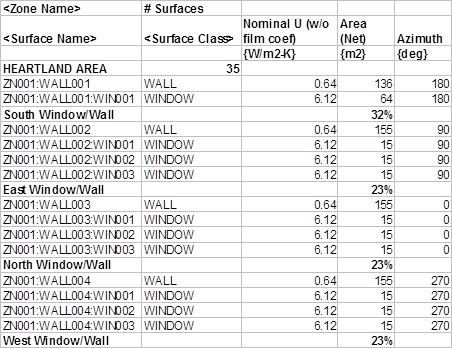
\includegraphics[width=0.9\textwidth, height=0.9\textheight, keepaspectratio=true]{media/image012.png}
\caption{Surface Details with Window/Wall \% calculated \protect \label{fig:surface-details-with-windowwall-calculated}}
\end{figure}

\subsection{Surface Convection Parameters}\label{surface-convection-parameters}

When detailed surface reports are requested, extra information on the surfaces related to how convection coefficients are calculated are also output to the EIO file.~ The first block of data relates to overall geometry parameters assigned to each surface and has the following header

! \textless{}Surface Convection Parameters\textgreater{}, Surface Name, Outside Model Assignment , Outside Area {[}m2{]}, Outside Perimeter {[}m{]}, Outside Height {[}m{]}, Inside Model Assignment, Inside Height {[}cm{]}, Inside Perimeter Envelope {[}m{]}, Inside Hydraulic Diameter {[}m{]}, Window Wall Ratio {[} {]},Window Location {[} {]}, Near Radiant {[}T/F{]}, Has Active HVAC {[}T/F{]}

With example data record.

Surface Convection Parameters,PERIMETER\_ZN\_1\_WALL\_SOUTH,0,84.45,61.48,3.05,0,3.05,27.69,6.94,0.24,0, F, F

\subsubsection{Field: Outside Model Assignment}\label{field-outside-model-assignment}

This is an integer code for the type of model assigned to the outside face, if a specific model has been assigned. Surface(SurfLoop)\%ExtConvCoeff

\begin{longtable}[c]{p{1.5in}p{4.5in}}
\toprule
Code value & meaning \tabularnewline
\midrule
\endfirsthead

\toprule
Code value & meaning \tabularnewline
\midrule
\endhead

0 & Not set special for this surface \tabularnewline
+/-1 & Simplest ASHRAE model \tabularnewline
+/-2 & TARP, ASHRAE-Walton model \tabularnewline
+/-5 & TARP, ASHRAE-Walton model \tabularnewline
+/- 6 & MoWITT model \tabularnewline
+/- 7 & DOE-2 model \tabularnewline
+/- 9 & Adaptive Convection Algorithm \tabularnewline
> 9 & Key values are indexes that are associated with the input order of SurfaceProperty:ConvectionCoefficients ( and MultipleSurface) \tabularnewline
\bottomrule
\end{longtable}

\subsubsection{Field: Outside Area}\label{field-outside-area}

This is the area used for convection calculations for the outside face.~ It is intended to be a model of the area of the larger group of surfaces that this surfaces is a part of. {[}m\(^{2}\){]}

\subsubsection{Field Outside Perimeter}\label{field-outside-perimeter}

This is the length of edge used for convection calculations for the outside face.~ It is intended to be a model of the perimeter for a larger group of surfaces that surface is a part of.~ {[}m{]}

\subsubsection{Field: Outside Height}\label{field-outside-height}

This is the height scale used for convection calculations for the outside face.~ It is intended to be a model of the overall height of a larger group of surfaces that this surface is a part of. {[}m{]}

\subsubsection{Field: Inside Model Assignment}\label{field-inside-model-assignment}

~This is an integer code for the type of model assigned to the inside face, if a specific model has been assigned. Surface(SurfLoop)\%IntConvCoeff

\subsubsection{Field: Inside Height}\label{field-inside-height}

This is the height scale used for convection calculations for the inside face.~ It is intended to be for the entire zone. {[}m{]}

\subsubsection{Field: Inside Perimeter Envelope}\label{field-inside-perimeter-envelope}

This is the length scale for the zone for the amount of exterior envelope with glazing.~ It is the length of wall that has glazed exterior.{[}m{]}

\subsubsection{Field: Inside Hydraulic Diameter}\label{field-inside-hydraulic-diameter}

This is the length scale for horizontal surfaces in the zone.~~ It is calculated using 4 * area/ perimeter and is used for natural convection on the floor or ceiling. {[}m{]}

\subsubsection{Field: Window to Wall Ratio}\label{field-window-to-wall-ratio}

This is the ratio of exterior window area to exterior wall area.~ It is for the zone. {[}non dimensional{]}

\subsubsection{Field: Window Location}\label{field-window-location}

This is an integer code for relative window positioning.~ It is used for some inside face correlations.

\subsubsection{Field: Near Radiant}\label{field-near-radiant}

This is a true or false flag indicating if this surfaces is near a radiant HVAC unit. If ``T'' then surface is is modeled as near a radiant HVAC device.~ If~ ``F'' then surface is normal.

\subsubsection{Field: Has Active HVAC}\label{field-has-active-hvac}

This is a true or false flag indicating if this surface has active HVAC elements inside it.~ If ``T'' then surface is modeled has having HVAC pipes or element inside it making it active for heating or cooling.~ If~ ``F'' then surface is normal.

\subsection{OtherSideCoefficient Outputs}\label{othersidecoefficient-outputs}

For the most part, the output for the Other Side Coefficients represents the input as entered. The header record for the Other Side Coefficients output is shown below:

\textbf{Line 1:} ! Other Side Coefficients,Name,Combined convective/radiative film coefficient,User selected Constant Temperature,Coefficient modifying the constant temperature term,Coefficient modifying the external dry bulb temperature term,Coefficient modifying the ground temperature term,Coefficient modifying the wind speed term \{s/m\},Coefficient modifying the zone air temperature term,Constant Temperature Schedule Name

\subsubsection{Field: Other Side Coefficients}\label{field-other-side-coefficients}

This field will be filled with the text \textbf{OtherSideCoefficients}.

The report describes the actions for the following equation:

The coefficients listed above are used in the following equation:

\begin{equation}
T = C_2 T_{zone} + C_3 T_{oadb} + C_4 C_5 + C_6 T_{grnd} + C_7 W_{spd} T_{oadb}
\end{equation}

where:

\begin{itemize}
\tightlist
\item
  T = Outdoor air Temperature when Combined convective/radiative film Coeff \textgreater{} 0
\item
  T = Exterior Surface Temperatre when Combined convective/radiative film Coeff \textless{} = 0
\item
  Tzone~ = Temperature of the zone being simulated (°C)
\item
  Toadb~ = Dry-bulb temperature of the outdoor air (°C)
\item
  Tgrnd~ = Temperature of the ground (°C)
\item
  Wspd~ = Outdoor wind speed (m/sec)
\end{itemize}

\subsubsection{Field: Name}\label{field-name-11}

This is the unique name entered for the OtherSideCoefficient. Note that the surface it applies to will have this name in the \textless{}ExtBoundCondition\textgreater{} field.

\subsubsection{Field: Combined convective/radiative film coefficient}\label{field-combined-convectiveradiative-film-coefficient}

This field is a trigger value. When entered as \textgreater{}0, it is used as the combined convective/radiative film coefficient. The other fields in the OtherSideCoefficient object are used then as well: the remaining fields are used first to calculate the outdoor air temperature for the surface and then to calculate the outside surface temperature based on the outdoor air temperature and the film coefficient. If this field contains \textbf{N/A}, then the remaining fields are used to calculate the surface temperature (not the outdoor air temperature).

\subsubsection{Field: User selected Constant Temperature}\label{field-user-selected-constant-temperature}

This field is a temperature that remains a constant part of the calculation either of the surface or outdoor air temperature. When the schedule option is used, this field will show \textbf{N/A}. The parameter in the equation for this or the schedule value is \textbf{\emph{C5}}.

\subsubsection{Field: Coefficient modifying the constant temperature term}\label{field-coefficient-modifying-the-constant-temperature-term}

This field is multiplied to the previous field when a simple number is entered. This parameter is shown as \textbf{\emph{C4}} in the equation. This parameter is dimensionless. The value of this parameter should be 1.0 if a schedule is used to set \textbf{\emph{C5}}.

\subsubsection{Field: Coefficient modifying the external dry bulb temperature term}\label{field-coefficient-modifying-the-external-dry-bulb-temperature-term}

This field defines a constant coefficient that is applied to the outdoor air dry-bulb temperature. This parameter is shown as \textbf{\emph{C3}} in the equation. This parameter is dimensionless.

\subsubsection{Field: Coefficient modifying the ground temperature term}\label{field-coefficient-modifying-the-ground-temperature-term}

This field defines a constant coefficient that is applied to the ground temperature. This parameter is shown as \textbf{\emph{C6}} in the equation. This parameter is dimensionless.

\subsubsection{Field: Coefficient modifying the wind speed term \{s/m\}}\label{field-coefficient-modifying-the-wind-speed-term-sm}

This field defines a constant coefficient that is applied to the product of the outdoor air dry-bulb temperature and the wind speed. This parameter is shown as \textbf{\emph{C7}} in the equation. This parameter has dimensions of inverse velocity or s/m.

\subsubsection{Field: Coefficient modifying the zone air temperature term}\label{field-coefficient-modifying-the-zone-air-temperature-term}

This field defines a constant coefficient that is applied to the temperature of the zone to which this surface belongs. This parameter is shown as \textbf{\emph{C2}} in the equation. This parameter is dimensionless.

\subsubsection{Field: Constant Temperature Schedule Name}\label{field-constant-temperature-schedule-name}

This field is used to supply a schedule name. That schedule supplies the ``constant'' temperature value \textbf{\emph{C5}}. Note that the value of the \textbf{\emph{C4}} field should normally be 1.0 if a schedule is used for \textbf{\emph{C5}}. If this field contains a value, then constant temperature field will be \textbf{N/A} in this report.

\subsection{Construction Element Outputs}\label{construction-element-outputs}

An optional report (contained in \textbf{eplusout.eio}) gives calculated elements for the materials and constructions used in the input. One report is specific to opaque constructions (note that nominal thermal conductance is calculated).

The report is invoked by including the following in the IDF:

\textbf{Output:Constructions,Constructions;}

\textbf{Line 1:}! \textless{}Construction\textgreater{},Construction Name,\#Layers,\#CTFs,Time Step \{hours\},ThermalConductance \{w/m2-K\},OuterThermalAbsorptance,InnerThermalAbsorptance,OuterSolarAbsorptance,InnerSolarAbsorptance,Roughness

\textbf{Line 2:}! \textless{}Material\textgreater{},Material Name,Thickness \{m\},Conductivity \{w/m-K\},Density \{kg/m3\},Specific Heat \{J/kg-K\},ThermalResistance \{m2-K/w\}

\textbf{Line 3:}! \textless{}Material:Air\textgreater{},Material Name,ThermalResistance \{m2-K/w\}

\textbf{Line 4:}! \textless{}CTF\textgreater{},Time,Outside,Cross,Inside,Flux (except final one)

\textbf{Ex Line 1:} Construction,EXTWALL09, 4,10, 0.250,2.545~~~ ,~~ 0.900,~~ 0.900,~~ 0.930,~~ 0.920,Rough

\textbf{Ex Line 2:} Material,A2 - 4 IN DENSE FACE BRICK,~ 0.1015, 1.245, 2082.400, 920.480,~ 0.8151E-01

\textbf{Ex Line 2:} Material:Air,B1 - AIRSPACE RESISTANCE,~ 0.1604

\textbf{Ex Line 2:} Material,C3 - 4 IN HW CONCRETE BLOCK,~ 0.1015, 0.813,~ 977.126,~ 836.800,~ 0.1249

\textbf{Ex Line 2:} Material,E1 - 3 / 4 IN PLASTER OR GYP BOARD,0.0191,0.726, 1601.846,~ 836.800,~ 0.2622E-01

\textbf{Ex Line 3:} CTF,~ 10,~~~~~ 0.13890138E-11,~~~~~ 0.95367648E-14,~~~~~ 0.62566281E-10,~~~~ -0.39500133E-14

\textbf{Ex Line 3:} CTF,~~ 9,~~~~ -0.32803336E-08,~~~~~ 0.29933755E-10,~~~~ -0.60855613E-07,~~~~~ 0.10196216E-10

\textbf{Ex Line 3:} CTF,~~ 8,~~~~~ 0.23798948E-05,~~~~~ 0.21201413E-07,~~~~~ 0.21649376E-04,~~~~ -0.88463084E-08

\textbf{Ex Line 3:} CTF,~~ 7,~~~~ -0.58681847E-03,~~~~~ 0.38118098E-05,~~~~ -0.26539198E-02,~~~~~ 0.25879187E-05

\textbf{Ex Line 3:} CTF,~~ 6,~~~~~ 0.46201324E-01,~~~~~ 0.18871269E-03,~~~~~ 0.12095720~~~ ,~~~~ -0.26290432E-03

\textbf{Ex Line 3:} CTF,~~ 5,~~~~~ -1.2828328~~~ ,~~~~~ 0.27337395E-02,~~~~~ -2.1646103~~~ ,~~~~~ 0.91268499E-02

\textbf{Ex Line 3:} CTF,~~ 4,~~~~~~ 13.603723~~~ ,~~~~~ 0.11920108E-01,~~~~~~ 17.065325~~~ ,~~~~ -0.12663354

\textbf{Ex Line 3:} CTF,~~ 3,~~~~~ -62.546625~~~ ,~~~~~ 0.15112689E-01,~~~~~ -64.276824~~~ ,~~~~~ 0.73877389

\textbf{Ex Line 3:} CTF,~~ 2,~~~~~~ 133.27916~~~ ,~~~~~ 0.47414487E-02,~~~~~~ 120.00640~~~ ,~~~~~ -1.9706501

\textbf{Ex Line 3:} CTF,~~ 1,~~~~~ -130.02410~~ ~,~~~~~ 0.22383019E-03,~~~~~ -106.88260~~~ ,~~~~~~ 2.3359193

\textbf{Ex Line 3:} CTF,~~ 0,~~~~~~ 46.959981~~~ ,~~~~~ 0.53137072E-06,~~~~~~ 36.168919~~~

\subsection{Opaque Constructions}\label{opaque-constructions}

\subsubsection{Description of the Opaque Construction Report}\label{description-of-the-opaque-construction-report}

The Opaque Construction report has 3 parts for each construction.

Part 1 is the construction name along with some derived values for the entire construction (i.e.~Thermal Conductance) as well as noting other details about the surface (\# CTFs, \#~ Layers).

Part 2 shows the material layers for the construction. This is essentially just an echo of the entered properties of the materials from the IDF.

Part 3 shows the CTFs as calculated for the Construction. CTFs are described more completely in the Engineering Reference document.

\subsubsection{Fields in Part 1 -- Opaque Construction Report}\label{fields-in-part-1-opaque-construction-report}

\subsubsection{Field: \textless{}Construction\textgreater{}}\label{field-construction-1}

This will be filled with the constant ``Construction'' for each Construction line.

\subsubsection{Field: Construction Name}\label{field-construction-name}

This is the name of the construction as entered in the IDF.

\subsubsection{Field: \#Layers}\label{field-layers}

This is the number of material layers inferred from the construction entry in the IDF. Material layers are listed ``outside'' to ``inside'' of the construction. This, of course, depends on the placement of the surface in the building -- the ``outside'' of an internal surface is the layer that is closest to whatever the surface touches whereas the ``inside'' of an internal surface is the layer that shows in the surface's ``zone''. The outside of an external surface is the layer that faces the outside environment and, again, the inside is the layer that shows in the zone.

\subsubsection{Field: \#CTFs}\label{field-ctfs}

This is the calculated number of CTFs (Conduction Transfer Functions). The conduction transfer functions are temperature and flux coefficients that characterize the thermal properties of the wall.

\subsubsection{Field: Time Step}\label{field-time-step}

The ``timestep'' in the construction line is the timestep at which the CTFs are valid. Because CTFs for certain constructions might not be stable at the user specified timestep (might be too ``heavy'' from a thermal mass standpoint), this may be different from the zone timestep (specified in ``TimeStep in Hour''). In all cases though, this will be greater than or equal to the zone timestep. If the timestep for the construction is greater than the zone timestep, E+ will use interpolated histories to solve for the surface heat balances for this surface (see discussion on interpolated histories in the \href{file:///E:/Docs4PDFs/EngineeringDoc.pdf}{Engineering Reference} document).

\subsubsection{Field: Thermal Conductance}\label{field-thermal-conductance}

This is the nominal thermal conductance of the construction calculated without film coefficients. Units are w/m\(^{2}\)-K.

\subsubsection{Field: Outer Thermal Absorptance}\label{field-outer-thermal-absorptance}

This will be the thermal absorptance of the outer material layer.

\subsubsection{Field: Inner Thermal Absorptance}\label{field-inner-thermal-absorptance}

This will be the thermal absorptance of the inner material layer.

\subsubsection{Field: Outer Solar Absorptance}\label{field-outer-solar-absorptance}

This will be the solar absorptance of the outer material layer.

\subsubsection{Field: Inner Solar Absorptance}\label{field-inner-solar-absorptance}

This will be the solar absorptance of the inner material layer.

\subsubsection{Field: Roughness}\label{field-roughness}

The construction takes on the roughness from the outer material layer. Roughness is used in several parts of external environment calculations.

\subsubsection{Fields in Part 2 -- Opaque Construction Report}\label{fields-in-part-2-opaque-construction-report}

\textbf{Line 2:} ! \textless{}Material\textgreater{},Material Name,Thickness \{m\},Conductivity \{w/m-K\},Density \{kg/m3\},Specific Heat \{J/kg-K\},ThermalResistance \{m2-K/w\}

In this version of part 2, the full material properties are entered by the user and displayed in the report.

\subsubsection{Field: \textless{}Material\textgreater{}}\label{field-material}

This will be filled with the constant ``Material'' for each material layer line.

\subsubsection{Field: Material Name}\label{field-material-name}

This is the name of the material as entered in the IDF.

\subsubsection{Field: Thickness}\label{field-thickness}

This is the entered thickness of the material. Units are m.

\subsubsection{Field: Conductivity}\label{field-conductivity}

For Material:Regular materials, this will be the entered conductivity in w/m-K. For Material:Regular-R materials, this will be shown as 0.0.

\subsubsection{Field: Density}\label{field-density}

For Material:Regular materials, this will be the entered density in kg/m\(^{3}\). For Material:Regular-R materials, this will be shown as 0.0.

\subsubsection{Field: Specific Heat}\label{field-specific-heat}

For Material:Regular materials, this will be the entered specific heat in J/kg-K. For Material:Regular-R materials, this will be shown as 0.0.

\subsubsection{Field: Thermal Resistance}\label{field-thermal-resistance}

For Material:Regular-R materials, this is the entered thermal resistance in m\(^{2}\)-K/w. For Material:Regular materials, this is the calculated thermal resistance based on the other properties.

\textbf{Line 3:} ! \textless{}Material:Air\textgreater{},Material Name,ThermalResistance \{m2-K/w\}

In this version of part 2, only the thermal resistance of the air layer is entered by the user and displayed in the report.

\subsubsection{Field: \textless{}Material:Air\textgreater{}}\label{field-materialair}

This will be filled with the constant ``Material:Air'' for each material layer line.

\subsubsection{Field: Material Name}\label{field-material-name-1}

This is the name of the material as entered in the IDF.

\subsubsection{Field: Thermal Resistance}\label{field-thermal-resistance-1}

This is the entered thermal resistance in m\(^{2}\)-K/w.

\subsubsection{Fields in Part 3 -- Opaque Construction Report}\label{fields-in-part-3-opaque-construction-report}

\textbf{Line 4:} ! \textless{}CTF\textgreater{},Time,Outside,Cross,Inside,Flux (except final one)

In part 3, the CTF calculations are shown. It is necessary to use the conduction transfer functions labeled ``Inside'' and ``Cross'' to calculate the heat flux at the inside surface and the conduction transfer functions labeled ``Outside'' and ``Cross'' to calculate the heat flux at the outside surface. Inside and outside coefficients will be identical for symmetric walls.

Conduction through constructions such as walls, roofs, floors, etc. is generally characterized as one-dimensional and transient within EnergyPlus. The solution to this partial differential equation results in ``conduction transfer functions'' or CTFs. In a CTF equation, the current heat transfer flux due to conduction through a construction is a function of the current temperature at either face of the surface as well as the history of temperatures at either face and the history of conductive fluxes at this face. CTFs are a simplification of response factors which are based solely on temperature histories and require an ``infinite'' history. The inclusion of heat flux history terms reduces the overall number of terms in the equation for conductive flux significantly, resulting in a more efficient solution.

For each unique combination of materials, there are a unique set of CTFs. While there are other procedures to determine the CTFs for a particular construction, EnergyPlus uses a state-space method (see conduction transfer function documentation) to obtain the CTF coefficients. These coefficients are calculated once at the beginning of the simulation and are constant for a particular construction. The CTF equation itself is a linear equation with these constant coefficients.

Conduction heat transfer flux at the outside face of a particular surface is a function of the construction of the surface (which leads to the CTF coefficients), the current and previous temperatures at both the inside and outside face of the surface, and the previous conduction heat transfer fluxes at the outside surface. The CTF coefficients that would be used in this equation would be the ``Outside'' (multiplied by the temperature history at the outside face) terms, the ``Cross'' (multiplied by the temperature history at the inside face) terms, and the ``Flux'' (multiplied by the flux history at the outside face) terms. Solving for the conductive flux at the inside surface would require the use of the ``Inside'' (multiplied by the temperature history at the inside face) terms, the ``Cross'' (multiplied by the temperature history at the outside face) terms, and the ``Flux'' (multiplied by the flux history at the inside face) terms. A textual example is given below for illustration purposes:

Current Outside Conductive Flux = (Outside Term 0) * (Current Outside Face Temperature)

~~~~~~~~~~~~~~~~~~~~~~~~~~~~~~~~ +(Outside Term 1) * (Previous Outside Face Temperature)

~~~~~~~~~~~~~~~~~~~~~~~~~~~~~~~~ +(Outside Term 2) * (Outside Face Temperature 2 Time Steps Ago)

~~~~~~~~~~~~~~~~~~~~~~~~~~~~~~~~ +(Outside Term 3) * (Outside Face Temperature 3 Time Steps Ago)

~~~~~~~~~~~~~~~~~~~~~~~~~~~~~~~~ + \ldots{}

~~~~~~~~~~~~~~~~~~~~~~~~~~~~~~~~ +(Cross Term 0) * (Current Inside Face Temperature)

~~~~~~~~~~~~~~~~~~~~~~~~~~~~~~~~ +(Cross Term 1) * (Previous Inside Face Temperature)

~~~~~~~~~~~~~~~~~~~~~~~~~~~~~~~~ +(Cross Term 2) * (Inside Face Temperature 2 Time Steps Ago)

~~~~~~~~~~~~~~~~~~~~~~~~~~~~~~~~ +(Cross Term 3) * (Inside Face Temperature 3 Time Steps Ago)

~~~~~~~~~~~~~~~~~~~~~~~~~~~~~~~~ + \ldots{}

~~~~~~~~~~~~~~~~~~~~~~~~~~~~~~~~ +(Flux Term 1) * (Previous Outside Face Flux)

~~~~~~~~~~~~~~~~~~~~~~~~~~~~~~~~ +(Flux Term 2) * (Outside Face Flux 2 Time Steps Ago)

~~~~~~~~~~~~~~~~~~~~~~~~~~~~~~~~ +(Flux Term 3) * (Outside Face Flux 3 Time Steps Ago)

~~~~~~~~~~~~~~~~~~~~~~~~~~~~~~~~ + \ldots{}

The number of terms is based on the CTF coefficient calculation routine and is related to the amount of thermal mass contained within a particular construction. Actual signs (positive or negative) of various terms in the preceding equation will vary based on their definition and use within the equation. Those interested in more details on the use and calculation of CTFs are encouraged to read the Engineering Documentation.

\subsubsection{Field: \textless{}CTF\textgreater{}}\label{field-ctf}

This will be filled with the constant ``CTF'' for each CTF coefficient line.

\subsubsection{Field: Time}\label{field-time}

This field ``time'' refers to the history term to which the coefficients are applied. The last line is the ``zero'' term that gets applied to the current values of temperatures. The line with a ``1'' refers to the temperatures and fluxes from the previous timestep--previous as in time minus one timestep. Timestep, in this case, is defined by the construction timestep (see description on ``Fields in Part 1 -- Opaque Construction Report'') \emph{not} the zone timestep. Lines with other values are for previous timesteps at t-n(timestep). These are the terms that are used to model conduction through a construction.

\subsubsection{Field: Outside}\label{field-outside}

\subsubsection{Field: Cross}\label{field-cross}

\subsubsection{Field: Inside}\label{field-inside}

\subsubsection{Field: Flux (except final one)}\label{field-flux-except-final-one}

\subsection{Window Constructions}\label{window-constructions}

\subsubsection{Description of the Windows Construction Report}\label{description-of-the-windows-construction-report}

A separate report is available for windows (note that both nominal conductance and Solar Heat Gain Coefficient are calculated for windows). Like the opaque construction, the window construction report has multiple parts -- in this case, 2.

\textbf{Line 1:} ! \textless{}WindowConstruction\textgreater{},Construction Name,\#Layers,Roughness,Conductance \{W/m2-K\},SHGC,SolarTransmittanceNormalIncid,VisibleTransmittanceNormalIncid

\textbf{Line 2:} ! \textless{}WindowMaterial:Glazing\textgreater{}, Material Name, Optical Data Type, Spectral Data Set Name, Thickness \{m\}, Solar Transmittance,Front Solar Reflectance, Back Solar Reflectance, Visible Transmittance, Front Visible Reflectance,Back Visible Reflectance,Infrared Transmittance, Front Thermal Emissivity, Back Thermal Emissivity,Conductivity \{W/m-K\},Dirt Factor,Solar Diffusing

\textbf{Line 3:} ! \textless{}WindowMaterial:Gas\textgreater{},Material Name,GasType,Thickness \{m\}

\textbf{Line 4:} ! \textless{}WindowMaterial:Shade\textgreater{},Material Name,Thickness \{m\},Conductivity \{W/m-K\},ThermalAbsorptance,Transmittance,VisibleTransmittance,ShadeReflectance

\textbf{Line 5:} ! \textless{}WindowMaterial:Screen\textgreater{},Material Name,Thickness \{m\},Conductivity \{W/m-K\},ThermalAbsorptance,Transmittance,Reflectance,VisibleReflectance,DiffuseReflectance,DiffuseVisibleReflectance,ScreenMaterialDiameterToSpacingRatio,ScreenToGlassDistance \{m\}

\textbf{Line 6:} ! \textless{}WindowMaterial:Blind\textgreater{},Material Name,SlatWidth \{m\},SlatSeparation \{m\},SlatThickness \{m\},SlatAngle \{deg\},SlatBeamSolarTransmittance,SlatBeamSolarFrontReflectance,BlindToGlassDistance \{m\}

WindowConstruction,DOUBLE PANE WITH SCREEN,~~ 4,MediumRough,~~ 2.514,~~ 0.555,~~ 0.511,~~ 0.589

~WindowMaterial:Screen,BRIGHT ALUMINUM SCREEN 1, 0.00025,~ 2.210E+02,~ 0.272,~ 0.697,~ 0.166,~ 0.166,~ 0.195,~ 0.195,~ 0.165,~ 0.025

~WindowMaterial:Glazing,GLASS - CLEAR SHEET 1 / 8 IN,SpectralAverage,,~ 0.00300,~ 0.83700,~ 0.07500,~ 0.07500,~ 0.89800,~ 0.08100,~ 0.08100,~ 0.00000,~ 0.84000,~ 0.84000,~ 0.90000,~ 1.00000,No

~WindowMaterial:Gas,WINAIRB1 - AIRSPACE RESISTANCE,Air,~ 1.300E-02,

~WindowMaterial:Glazing,GLASS - CLEAR SHEET 1 / 8 IN,SpectralAverage,,~ 0.00300,~ 0.83700,~ 0.07500,~ 0.07500,~ 0.89800,~ 0.08100,~ 0.08100,~ 0.00000,~ 0.84000,~ 0.84000,~ 0.90000,~ 1.00000,No

WindowConstruction,DOUBLE PANE WITH SHADE,~~ 4,VerySmooth,~~ 2.716,~~ 0.482,~~ 0.039,~~ 0.050

~WindowMaterial:Glazing,GLASS - CLEAR SHEET 1 / 8 IN,SpectralAverage,,~ 0.00300,~ 0.83700,~ 0.07500,~ 0.07500,~ 0.89800,~ 0.08100,~ 0.08100,~ 0.00000,~ 0.84000,~ 0.84000,~ 0.90000,~ 1.00000,No

~WindowMaterial:Gas,WINAIRB1 - AIRSPACE RESISTANCE,Air,~ 1.300E-02,

~WindowMaterial:Glazing,GLASS - CLEAR SHEET 1 / 8 IN,SpectralAverage,,~ 0.00300,~ 0.83700,~ 0.07500,~ 0.07500,~ 0.89800,~ 0.08100,~ 0.08100,~ 0.00000,~ 0.84000,~ 0.84000,~ 0.90000,~ 1.00000,No

~WindowMaterial:Shade,SHADE ROLL - LIGHT OPAQUE,~ 0.003,~ 1.000E-01,~ 0.900,~ 0.050,~ 0.050,~ 0.500

WindowConstruction,DOUBLE PANE WITH BLIND,~~ 4,VerySmooth,~~ 2.761,~~ 0.714,~~ 0.395,~~ 0.456

~WindowMaterial:Glazing,GLASS - CLEAR SHEET 1 / 8 IN,~ 0.003,~ 0.900,~ 0.837,~ 0.898,~ 0.840,~ 0.840,~ 0.075,~ 0.075,~ 0.081,~ 0.081,~ 1.000,NO

~WindowMaterial:Gas,WINAIRB1 - AIRSPACE RESISTANCE,Air,~ 1.300E-02,

~WindowMaterial:Glazing,GLASS - CLEAR SHEET 1 / 8 IN,~ 0.003,~ 0.900,~ 0.837,~ 0.898,~ 0.840,~ 0.840,~ 0.075,~ 0.075,~ 0.081,~ 0.081,~ 1.000,NO

~WindowMaterial:Blind,INTERIOR BLIND, 0.0010, 0.0022, 0.0010,~ 0.000,~ 0.000,~ 0.200,~ 0.025

\subsubsection{Fields in Part 1 -- Window Construction Report}\label{fields-in-part-1-window-construction-report}

\textbf{Line 1:} ! \textless{}WindowConstruction\textgreater{},Construction Name,\#Layers,Roughness,Conductance \{W/m2-K\},SHGC,SolarTransmittanceNormalIncid,VisibleTransmittanceNormalIncid

\subsubsection{Field: \textless{}WindowConstruction\textgreater{}}\label{field-windowconstruction}

This will be filled with the constant ``Construction'' for each Window Construction line.

\subsubsection{Field: Construction Name}\label{field-construction-name-1}

This is the name of the window as entered in the IDF.

\subsubsection{Field: \#Layers}\label{field-layers-1}

This is the number of material layers inferred from the windows construction entry in the IDF. Material layers are listed ``outside'' to ``inside'' of the construction. This, of course, depends on the placement of the surface in the building -- the ``outside'' of an internal surface is the layer that is closest to whatever the surface touches whereas the ``inside'' of an internal surface is the layer that shows in the surface's ``zone''. The outside of an external surface is the layer that faces the outside environment and, again, the inside is the layer that shows in the zone.

\subsubsection{Field: Roughness}\label{field-roughness-1}

The window construction takes on the roughness from the outer material layer. Roughness is used in several parts of external environment calculations.

\subsubsection{Field: Conductance}\label{field-conductance}

This is the center-of-glass conductance of the construction calculated with film coefficients, for winter conditions (indoor air temperature = 21C (69.8F), outdoor air temperature = -18C (-.4F), windspeed = 5.5 m/s (12.3 mph), no solar radiation). Units are W/m\(^{2}\)-K.

\subsubsection{Field: SHGC}\label{field-shgc}

This is the center-of-glass Solar Heat Gain Coefficient for summer conditions (indoor air temperature = 24C (75.2F), outdoor air temperature = 32C (89.6F), windspeed = 2.8 m/s (6.2 mph), 783 W/m2 (248 Btu/h-ft2) incident beam solar radiation normal to glazing.

The following transmittance and reflectance values are for the window glazing (plus shade, screen or blind, if present in the construction). For exterior windows, ``front'' means the side of the window facing the exterior environment and ``back'' means the side facing the zone. For interior windows, ``front'' means the side to window facing the zone and ``back'' means the side facing the adjacent zone.

\subsubsection{Field: Solar Transmittance at Normal Incidence (SolarTransmittanceNormalIncid)}\label{field-solar-transmittance-at-normal-incidence-solartransmittancenormalincid}

Transmittance at normal incidence averaged over the solar spectrum.

\subsubsection{Field: Visible Transmittance at Normal Incidence (VisibleTransmittanceNormalIncid)}\label{field-visible-transmittance-at-normal-incidence-visibletransmittancenormalincid}

Transmittance normal incidence averaged over the solar spectrum and weighted by the response of the human eye.

\subsubsection{Fields in Part 2 -- Window Construction Report}\label{fields-in-part-2-window-construction-report}

Part 2 of the Window Construction Report encompasses several ``lines''.

\textbf{Line 2:} ! \textless{}WindowMaterial:Glazing\textgreater{}, Material Name, Optical Data Type, Spectral Data Set Name, Thickness \{m\}, Solar Transmittance,Front Solar Reflectance, Back Solar Reflectance, Visible Transmittance, Front Visible Reflectance,Back Visible Reflectance,Infrared Transmittance, Front Thermal Emissivity, Back Thermal Emissivity,Conductivity \{W/m-K\},Dirt Factor,Solar Diffusing

\textbf{Line 3:} ! \textless{}WindowMaterial:Gas\textgreater{},Material Name,GasType,Thickness \{m\}

\textbf{Line 4:} ! \textless{}WindowMaterial:Shade\textgreater{},Material Name,Thickness \{m\},Conductivity \{W/m-K\},ThermalAbsorptance,Transmittance,VisibleTransmittance,ShadeReflectance

\textbf{Line 5:} ! \textless{}WindowMaterial:Screen\textgreater{},Material Name,Thickness \{m\},Conductivity \{W/m-K\},ThermalAbsorptance,Transmittance,Reflectance,VisibleReflectance,DiffuseReflectance,DiffuseVisibleReflectance,ScreenMaterialDiameterToSpacingRatio,ScreenToGlassDistance \{m\}

\textbf{Line 6:} ! \textless{}WindowMaterial:Blind\textgreater{},Material Name,SlatWidth \{m\},SlatSeparation \{m\},SlatThickness \{m\},SlatAngle \{deg\},SlatBeamSolarTransmittance,SlatBeamSolarFrontReflectance,BlindToGlassDistance \{m\}

\subsection{Material\textbf{:}WindowGlass}\label{materialwindowglass}

\subsubsection{Field:~ \textless{}Material:WindowGlass\textgreater{}}\label{field-materialwindowglass}

This will be filled with the constant ``Material:WindowGlass'' for each material of this type in the construction.

\subsubsection{Field: Material Name}\label{field-material-name-2}

Name of the glass layer.

\subsubsection{Field: Thickness \{m\}}\label{field-thickness-m}

Thickness of the glass layer.

\subsubsection{Field: Conductivity \{w/m-K\}}\label{field-conductivity-wm-k}

Conductivity of the glass layer.

\subsubsection{Field: SolarTransmittance}\label{field-solartransmittance}

Transmittance of the glass layer at normal incidence averaged over the solar spectrum.

\subsubsection{Field: VisibleTransmittance}\label{field-visibletransmittance}

Transmittance normal incidence of the glass layer averaged over the solar spectrum and weighted by the response of the human eye.

\subsubsection{Field: ThermalFrontAbsorptance}\label{field-thermalfrontabsorptance}

Thermal emissivity of the front face of the glass layer.

\subsubsection{Field: ThermalBackAbsorptance}\label{field-thermalbackabsorptance}

Thermal emissivity of the back face of the glass layer.

\subsubsection{Field: SolarFrontReflectance}\label{field-solarfrontreflectance}

Reflectance of the front face of the glass layer at normal incidence averaged over the solar spectrum.

\subsubsection{Field: SolarBackReflectance}\label{field-solarbackreflectance}

Reflectance of the back face of the glass layer at normal incidence averaged over the solar spectrum.

\subsubsection{Field: VisibleFrontReflectance}\label{field-visiblefrontreflectance}

Reflectance of the front face of the glass layer at normal incidence averaged over the solar spectrum.

\subsubsection{Field: VisibleBackReflectance}\label{field-visiblebackreflectance}

Reflectance of the back face of the glass layer at normal incidence averaged over the solar spectrum.

\subsubsection{Field: GlassTransDirtFactor}\label{field-glasstransdirtfactor}

Glass transmittance dirt factor (1.0 is clear, no dirt factor).

\subsubsection{Field: SolarDiffusing}\label{field-solardiffusing}

Solar Diffusing value -- Yes if solar diffusing glass, No if not.

\subsubsection{Material:WindowGas}\label{materialwindowgas}

\subsubsection{Field:~ \textless{}Material:WindowGas\textgreater{}}\label{field-materialwindowgas}

This will be filled with the constant ``Material:WindowGas'' for each material of this type in the construction.

\subsubsection{Field: Material Name}\label{field-material-name-3}

Name of the gas layer.

\subsubsection{Field: GasType}\label{field-gastype}

Type of the gas layer. Possibilities are Air, Argon, Krypton,~ Xenon, and Custom.

\subsubsection{Field: Thickness \{m\}}\label{field-thickness-m-1}

Thickness of the gas layer.

\subsubsection{Material:WindowShade}\label{materialwindowshade}

\subsubsection{Field:~ \textless{}Material:WindowShade\textgreater{}}\label{field-materialwindowshade}

This will be filled with the constant ``Material:WindowShade'' for each material of this type in the construction.

\subsubsection{Field: Material Name}\label{field-material-name-4}

Name of the window shade layer.

\subsubsection{Field: Thickness \{m\}}\label{field-thickness-m-2}

Thickness of the window shade layer.

\subsubsection{Field: Conductivity \{w/m-K\}}\label{field-conductivity-wm-k-1}

Thermal conductivity of the window shade layer.

\subsubsection{Field: ThermalAbsorptance}\label{field-thermalabsorptance}

Emissivity of the window shade layer (assumed same for front and back faces).

\subsubsection{Field: SolarTransmittance}\label{field-solartransmittance-1}

Transmittance of the window shade layer averaged over the solar spectrum. Assumed same for beam solar radiation and diffuse solar radiation. Transmittance of beam solar radiation is assumed to be independent of angle of incidence.

\subsubsection{Field: VisibleTransmittance}\label{field-visibletransmittance-1}

Transmittance of the window shade layer averaged over the solar spectrum and weighted by the response of the human eye. Assumed same for beam visible radiation and diffuse visible radiation. Transmittance of beam visible radiation is assumed to be independent of angle of incidence.

\subsubsection{Field: ShadeReflectance}\label{field-shadereflectance}

Reflectance of the window shade layer averaged over the solar spectrum. Assumed same for beam solar radiation and diffuse solar radiation. Reflectance of beam solar radiation is assumed to be independent of angle of incidence. Reflectance is assumed to be the same for the front and back faces of the shade layer.

\subsection{Material:WindowBlind}\label{materialwindowblind}

This will be filled with the constant ``Material:WindowBlind'' for each material of this type in the construction.

\subsubsection{Field: \textless{}Material:WindowBlind\textgreater{}}\label{field-materialwindowblind}

\subsubsection{Field: Material Name}\label{field-material-name-5}

Name of the blind layer.

\subsubsection{Field: SlatWidth \{m\}}\label{field-slatwidth-m}

Width of the slats in the blind.

\subsubsection{Field: SlatSeparation \{m\}}\label{field-slatseparation-m}

Distance between the centerline of adjacent slats.

\subsubsection{Field: SlatThickness \{m\}}\label{field-slatthickness-m}

Distance between front and back faces of a slat.

\subsubsection{Field: SlatAngle \{deg\}}\label{field-slatangle-deg}

This is the angle between the glazing outward normal and the slat outward normal, where the outward normal points away from the front face of the slat.

\subsubsection{Field: SlatBeamSolarTransmittance}\label{field-slatbeamsolartransmittance}

The beam solar transmittance of the slat at normal incidence. Any transmitted beam radiation is assumed to be 100\% diffuse (i.e., slats are translucent). Transmittance is assumed to have the same value at other angles of incidence.

\subsubsection{Field: SlatBeamSolarFrontReflectance}\label{field-slatbeamsolarfrontreflectance}

The beam solar reflectance at normal incidence on the front side of the slat. Assumed to have the same value at other angles of incidence (matte finish).

\subsubsection{Field: BlindToGlassDistance \{m\}}\label{field-blindtoglassdistance-m}

Distance from the mid-plane of the blind to the adjacent glass (m).

\subsubsection{Material:WindowScreen}\label{materialwindowscreen}

\subsubsection{Field:~ \textless{}Material:WindowScreen\textgreater{}}\label{field-materialwindowscreen}

This will be filled with the constant ``Material:WindowScreen'' for each material of this type in the construction.

\subsubsection{Field: Material Name}\label{field-material-name-6}

Name of the window screen layer.

\subsubsection{Field: Thickness \{m\}}\label{field-thickness-m-3}

Thickness of the window screen layer (screen material diameter).

\subsubsection{Field: Conductivity \{w/m-K\}}\label{field-conductivity-wm-k-2}

Thermal conductivity of the window screen layer. This is the effective value for the overall screen ``assembly'' including open spaces between the screen material.

\subsubsection{Field: ThermalAbsorptance}\label{field-thermalabsorptance-1}

Emissivity of the window screen layer (assumed same for front and back faces). This is the effective value for the overall screen ``assembly'' including open spaces between the screen material.

\subsubsection{Field: Transmittance}\label{field-transmittance}

Beam transmittance of the window screen layer including any inward reflections from the material surface if specified (i.e., Material: WindowScreen, field Reflected Beam Transmittance Accounting Method). This is the effective value for the overall screen ``assembly'' including open spaces between the screen material. The value reported here is for direct normal incidence.

\subsubsection{Field: Reflectance}\label{field-reflectance}

Solar reflectance (beam-to-diffuse) of the window screen layer accounting for inward-reflected beam solar radiation as specified (i.e., Material: WindowScreen, field Reflected Beam Transmittance Accounting Method). This is the effective value for the overall screen ``assembly'' including open spaces between the screen material averaged over the solar spectrum. The value reported here is for direct normal incidence.

\subsubsection{Field: VisibleReflectance}\label{field-visiblereflectance}

Visible reflectance (beam-to-diffuse) of the window screen layer accounting for inward-reflected beam solar radiation as specified (i.e., Material: WindowScreen, field Reflected Beam Transmittance Accounting Method). This is the effective value for the overall screen ``assembly'' including open spaces between the screen material averaged over the solar spectrum and weighted by the response of the human eye. The value reported here is for direct normal incidence.

\subsubsection{Field: DiffuseReflectance}\label{field-diffusereflectance}

Solar reflectance (diffuse-to-diffuse) of the window screen layer accounting for inward-reflected beam solar radiation as specified (i.e., Material: WindowScreen, field Reflected Beam Transmittance Accounting Method). Reflectance of diffuse solar radiation is considered constant and applies to both the front and back surfaces of the screen. Diffuse reflectance is calculated by the model as an average value by integrating the screen's solar reflectance (beam-to-diffuse) over a quarter hemisphere of incident radiation.

\subsubsection{Field: DiffuseVisibleReflectance}\label{field-diffusevisiblereflectance}

Visible reflectance (diffuse-to-diffuse) of the window screen layer accounting for inward-reflected beam solar radiation as specified (i.e., Material: WindowScreen, field Reflected Beam Transmittance Accounting Method). Visible reflectance of diffuse solar radiation is considered constant and applies to both the front and back surfaces of the screen. Diffuse visible reflectance is calculated by the model as an average value by integrating the screen's visible beam reflectance (beam-to-diffuse) over a quarter hemisphere of incident radiation.

\subsubsection{Field: ScreenMaterialDiameterToSpacingRatio}\label{field-screenmaterialdiametertospacingratio}

The aspect ratio of the screen material. The aspect ratio is calculated as the ratio of the screen material diameter to screen material spacing.

\subsubsection{Field: ScreenToGlassDistance \{m\}}\label{field-screentoglassdistance-m}

Distance from the mid-plane of the screen to the adjacent glass (m).

\subsection{ThermoChromic Windows}\label{thermochromic-windows}

Windows with Thermochromic constructions are reported similarly to other window constructions. First, you see the window as entered in the IDF:

WindowConstruction,TCWINDOW,~~ 5,VerySmooth,~~ 1.666,~~ 0.429,~~ 0.242,~~ 0.520

~WindowMaterial:Glazing,CLEAR3PPG,Spectral,CLEAR3PPGSP,~ 0.00328,~ 0.00000,~ 0.00000,~ 0.00000,~ 0.00000,~ 0.00000,~ 0.00000,~ 0.00000,~ 0.84000,~ 0.84000,~ 1.00000,~ 1.00000,No

~WindowMaterial:Gas,AIR 3MM,Air,~ 3.000E-03,

~WindowMaterial:Glazing,WO18RT25,Spectral,WO18RT25SP,~ 0.00750,~ 0.00000,~ 0.00000,~ 0.00000,~ 0.00000,~ 0.00000,~ 0.00000,~ 0.00000,~ 0.84000,~ 0.84000,~ 0.60000,~ 1.00000,No

~WindowMaterial:Gas,AIR 8MM,Air,~ 8.000E-03,

~WindowMaterial:Glazing,SB60CLEAR3PPG,Spectral,SB60CLEAR3PPGSP,~ 0.00328,~ 0.00000,~ 0.00000,~ 0.00000,~ 0.00000,~ 0.00000,~ 0.00000,~ 0.00000,~ 0.03500,~ 0.84000,~ 1.00000,~ 1.00000,No

Then, there will be a list of window constructions reported with each one corresponding to a particular temperature of the thermochromic glazing layer. For example, the following excerpt shows a list of window constructions for the thermochromic window TCWINDOW at different temperature of the thermochromic layer - TCWINDOW\_TC\_25 at 25°C, TCWINDOW\_TC\_27 at 27°C, and TCWINDOW\_TC\_29 at 29°C. Detailed properties of the thermochromic glazing layer are also listed for each temperature - WO18RT25 \textbf{at} 25°C, WO18RT27 \textbf{at} 27°C, and WO18RT29 \textbf{at} 29°C.

WindowConstruction,TCWINDOW\_TC\_25,~~ 5,VerySmooth,~~ 1.666,~~ 0.429,~~ 0.242,~~ 0.520

~WindowMaterial:Glazing,CLEAR3PPG,Spectral,CLEAR3PPGSP,~ 0.00328,~ 0.00000,~ 0.00000,~ 0.00000,~ 0.00000,~ 0.00000,~ 0.00000,~ 0.00000,~ 0.84000,~ 0.84000,~ 1.00000,~ 1.00000,No

~WindowMaterial:Gas,AIR 3MM,Air,~ 3.000E-03,

~WindowMaterial:Glazing,WO18RT25,Spectral,WO18RT25SP,~ 0.00750,~ 0.00000,~ 0.00000,~ 0.00000,~ 0.00000,~ 0.00000,~ 0.00000,~ 0.00000,~ 0.84000,~ 0.84000,~ 0.60000,~ 1.00000,No

~WindowMaterial:Gas,AIR 8MM,Air,~ 8.000E-03,

~WindowMaterial:Glazing,SB60CLEAR3PPG,Spectral,SB60CLEAR3PPGSP,~ 0.00328,~ 0.00000,~ 0.00000,~ 0.00000,~ 0.00000,~ 0.00000,~ 0.00000,~ 0.00000,~ 0.03500,~ 0.84000,~ 1.00000,~ 1.00000,No

~WindowConstruction,TCWINDOW\_TC\_27,~~ 5,VerySmooth,~~ 1.666,~~ 0.424,~~ 0.236,~~ 0.504

~WindowMaterial:Glazing,CLEAR3PPG,Spectral,CLEAR3PPGSP,~ 0.00328,~ 0.00000,~ 0.00000,~ 0.00000,~ 0.00000,~ 0.00000,~ 0.00000,~ 0.00000,~ 0.84000,~ 0.84000,~ 1.00000,~ 1.00000,No

~WindowMaterial:Gas,AIR 3MM,Air,~ 3.000E-03,

~WindowMaterial:Glazing,WO18RT27,Spectral,WO18RT27SP,~ 0.00750,~ 0.00000,~ 0.00000,~ 0.00000,~ 0.00000,~ 0.00000,~ 0.00000,~ 0.00000,~ 0.84000,~ 0.84000,~ 0.60000,~ 1.00000,No

~WindowMaterial:Gas,AIR 8MM,Air,~ 8.000E-03,

~WindowMaterial:Glazing,SB60CLEAR3PPG,Spectral,SB60CLEAR3PPGSP,~ 0.00328,~ 0.00000,~ 0.00000,~ 0.00000,~ 0.00000,~ 0.00000,~ 0.00000,~ 0.00000,~ 0.03500,~ 0.84000,~ 1.00000,~ 1.00000,No

~WindowConstruction,TCWINDOW\_TC\_29,~~ 5,VerySmooth,~~ 1.666,~~ 0.419,~~ 0.230,~~ 0.490

~WindowMaterial:Glazing,CLEAR3PPG,Spectral,CLEAR3PPGSP,~ 0.00328,~ 0.00000,~ 0.00000,~ 0.00000,~ 0.00000,~ 0.00000,~ 0.00000,~ 0.00000,~ 0.84000,~ 0.84000,~ 1.00000,~ 1.00000,No

~WindowMaterial:Gas,AIR 3MM,Air,~ 3.000E-03,

~WindowMaterial:Glazing,WO18RT29,Spectral,WO18RT29SP,~ 0.00750,~ 0.00000,~ 0.00000,~ 0.00000,~ 0.00000,~ 0.00000,~ 0.00000,~ 0.00000,~ 0.84000,~ 0.84000,~ 0.60000,~ 1.00000,No

~WindowMaterial:Gas,AIR 8MM,Air,~ 8.000E-03,

~WindowMaterial:Glazing,SB60CLEAR3PPG,Spectral,SB60CLEAR3PPGSP,~ 0.00328,~ 0.00000,~ 0.00000,~ 0.00000,~ 0.00000,~ 0.00000,~ 0.00000,~ 0.00000,~ 0.03500,~ 0.84000,~ 1.00000,~ 1.00000,No

\subsection{Complex Fenestration}\label{complex-fenestration}

Complex fenestration is reported in a similar manner as other windows.~ The first line is the header, followed by details about each fenestration object (window).

~! \textless{}WindowConstruction:Complex\textgreater{},Construction Name,Index,\#Layers,U-factor \{W/m2-K\},SHGC

~WindowConstruction:Complex,CFS\_GLZ\_813,6,4,0.544,9.104E-002

~WindowConstruction:Complex,CFS\_GLZ\_2015,7,3,1.777,9.205E-002

~WindowConstruction:Complex,CFS\_GLZ\_2046,8,3,2.418,9.273E-002

~WindowConstruction:Complex,CFS\_GLZ\_2001,9,3,1.989,9.253E-002

\subsubsection{Field: Construction Name}\label{field-construction-name-2}

Name of the complex fenestration construction.

\subsubsection{Field: Index}\label{field-index}

Index number in construction data.

\subsubsection{Field: \#Layers}\label{field-layers-2}

Number of solid layers in the complex fenestration construction.~ This number accounts for glass and shading layers.

\subsubsection{Field: U-factor}\label{field-u-factor}

Complex fenestration U-factor according to ASHRAE winter conditions.

\subsubsection{Field: SHGC}\label{field-shgc-1}

Complex fenestration solar heat gain coefficient according to ASHRAE summer conditions.

\subsection{HAMT Cell Data}\label{hamt-cell-data}

This gives the surface name,the construction name, the origins and cell numbers of the cells used within the HAMT solutions algorithm. The cell numbering starts from the external surface to the internal surface.

! \textless{}HAMT origins\textgreater{}, Surface Name, Construction Name, Cell origins (m)

! \textless{}HAMT cells\textgreater{}, Surface Name, Construction Name, Cell Numbers

HAMT origins,SOUTH WALL,EXTERIOR WALL, 0.0000000, 0.0005729,

0.0026459, 0.0060000, 0.0093541, 0.0114271, 0.0128076, 0.0159588,

0.0219528, 0.0302028, 0.0399012, 0.0500988, 0.0597972, 0.0680472,

0.0740412, 0.0771924, 0.0785729, 0.0806459, 0.0840000, 0.0873541,

0.0894271, 0.0900000

HAMT cells, SOUTH WALL,EXTERIOR

WALL,~~ 1,~~ 2,~~ 3,~~ 4,~~ 5,~~ 6,~~ 7,~~ 8,~~ 9,~ 10,~ 11,~ 12,

13,~ 14,~ 15,~ 16,~ 17,~ 18,~ 19,~ 20,~ 21,~ 22

\subsubsection{Field: Surface Name}\label{field-surface-name-1}

Name of the Surface.

\subsubsection{Field: Construction Name}\label{field-construction-name-3}

Name of the construction.

\subsubsection{Field: Cell origins}\label{field-cell-origins}

Origins of the Cells.

\subsubsection{Field: Cell Numbers}\label{field-cell-numbers}

Numbers for the Cells.

\subsection{Sizing Information}\label{sizing-information}

The sizing information in the .eio file reflects the inputs and results for the zone, system and plant (component). Actual fields/details included depend on the ``autosize'' inputs.

\subsubsection{Timesteps in Zone Design Calculation}\label{timesteps-in-zone-design-calculation}

\textbf{! \textless{}Load Timesteps in Zone Design Calculation Averaging Window\textgreater{}, Value}

~Load Timesteps in Zone Design Calculation Averaging Window,~~~ 1

\subsubsection{Field: Load Timesteps in Zone Design Calculation Averaging Window}\label{field-load-timesteps-in-zone-design-calculation-averaging-window}

The number of load timesteps in the zone design flow sequence averaging window. The default is 1, in which case the calculated zone design flow rates are averaged over the load timestep.

The zone design air flow rate calculation is performed assuming a potentially infinite supply of heating or cooling air at a fixed temperature. Thus, the calculated design air flow rate will always be able to meet any load or change in load no matter how large or abrupt. In reality air flow rates are limited by duct sizes and fan capacities. The idealized zone design flow calculation may result in unrealistically large flow rates, especially if the user is performing the sizing calculations using thermostat schedules with night setup or setback. The calculated zone design flow rates are always averaged over the load timestep. The user may want to perform a broader average to mitigate the effect of thermostat setup and setback and prevent the warm up or cool down flow rates from dominating the design flow rate calculation. Specifying the width of the averaging window allows the user to do this.

For example, if the load calculation timestep is 15 minutes and the user specifies the \emph{timesteps in averaging window}to be 4, the zone design air flows will be averaged over a time period of 1 hour. Specifying 8 would result in averaging over a 2 hour period.

\subsubsection{Sizing Factor Information}\label{sizing-factor-information}

\textbf{! \textless{}Sizing Factor Information\textgreater{}, Sizing Factor ID, Value}

Sizing Factor Information, Global,~~ 1.3000

~Sizing Factor Information, Zone SPACE1-1,~~ 1.3000

~Sizing Factor Information, Zone SPACE2-1,~~ 1.3000

~Sizing Factor Information, Zone SPACE3-1,~~ 1.3000

~Sizing Factor Information, Zone SPACE4-1,~~ 1.3000

~Sizing Factor Information, Zone SPACE5-1,~~ 1.3000

\subsubsection{Field: Sizing Factor ID}\label{field-sizing-factor-id}

Sizing factors can be entered in two places: Sizing Parameters, Zone Sizing. If entered in the Sizing Parameters statement, the Sizing Factor ID is ``Global'' (applied to all if not specified). If entered in the Zone Sizing statement, the Zone and Zone Name designation are shown.

This sizing factor ratio is applied at the zone level to all of the zone heating and cooling loads and air flow rates. These new loads and air flow rates are then used to calculate the system level flow rates and capacities and are used in all of the component sizing calculations.

\subsubsection{Field: Value}\label{field-value}

This is the sizing factor ratio to be applied as described previously.

\subsection{Zone Sizing Information}\label{zone-sizing-information}

! \textless{}Zone Sizing Information\textgreater{}, Zone Name, Load Type, Calc Des Load \{W\}, User Des Load \{W\}, Calc Des Air Flow Rate \{m3/s\}, User Des Air Flow Rate \{m3/s\}, Design Day Name, Date/Time of Peak, Temperature at Peak \{C\}, Humidity Ratio at Peak \{kgWater/kgAir\}, Floor Area \{m2\}, \# Occupants, Calc Outdoor Air Flow Rate \{m3/s\}

~Zone Sizing Information, SPACE1-1, Cooling, 2502.43786, 3253.16922, 0.21023, 0.27329, CHICAGO ANN CLG 1\% CONDNS DB = \textgreater{}MWB, 7/21 16:00:00, 30.85800, 1.45947E-002, 99.16000, 11.00000, 0.10384

~Zone Sizing Information, SPACE1-1, Heating, 2606.90880, 3388.98144, 7.56806E-002, 0.10384, CHICAGO ANN HTG 99\% CONDNS DB, 1/21 23:45:00, -17.30000, 8.38927E-004, 99.16000, 11.00000, 0.10384

~Zone Sizing Information, SPACE2-1, Cooling, 2038.79983, 2650.43978, 0.17125, 0.22263, CHICAGO ANN CLG 1\% CONDNS DB = \textgreater{}MWB, 7/21 10:15:00, 27.83525, 1.45947E-002, 42.73500, 5.00000, 4.72000E-002

~Zone Sizing Information, SPACE2-1, Heating, 1149.09174, 1493.81926, 3.33591E-002, 4.72000E-002, CHICAGO ANN HTG 99\% CONDNS DB, 1/21 24:00:00, -17.30000, 8.38927E-004, 42.73500, 5.00000, 4.72000E-002

~Zone Sizing Information, SPACE3-1, Cooling, 2318.10750, 3013.53976, 0.19473, 0.25315, CHICAGO ANN CLG 1\% CONDNS DB = \textgreater{}MWB, 7/21 15:00:00, 31.50000, 1.45947E-002, 96.48000, 11.00000, 0.10384

~Zone Sizing Information, SPACE3-1, Heating, 2589.95436, 3366.94067, 7.51884E-002, 0.10384, CHICAGO ANN HTG 99\% CONDNS DB, 1/21 23:30:00, -17.30000, 8.38927E-004, 96.48000, 11.00000, 0.10384

~Zone Sizing Information, SPACE4-1, Cooling, 2325.33534, 3022.93594, 0.19534, 0.25394, CHICAGO ANN CLG 1\% CONDNS DB = \textgreater{}MWB, 7/21 17:30:00, 29.46700, 1.45947E-002, 42.73500, 5.00000, 4.72000E-002

~Zone Sizing Information, SPACE4-1, Heating, 1143.87745, 1487.04068, 3.32077E-002, 4.72000E-002, CHICAGO ANN HTG 99\% CONDNS DB, 1/21 23:30:00, -17.30000, 8.38927E-004, 42.73500, 5.00000, 4.72000E-002

~Zone Sizing Information, SPACE5-1, Cooling, 2589.39474, 3366.21317, 0.21753, 0.28279, CHICAGO ANN CLG 1\% CONDNS DB = \textgreater{}MWB, 7/21 15:00:00, 31.50000, 1.45947E-002, 182.49000, 20.00000, 0.18880

~Zone Sizing Information, SPACE5-1, Heating, 1706.17191, 2218.02348, 4.95314E-002, 0.18880, CHICAGO ANN HTG 99\% CONDNS DB, 1/21 23:45:00, -17.30000, 8.38927E-004, 182.49000, 20.00000, 0.18880

\subsubsection{Field: \textless{}Zone Sizing Information\textgreater{}}\label{field-zone-sizing-information}

This field just contains ``Zone Sizing Information''.

\subsubsection{Field: Zone Name}\label{field-zone-name-11}

This field contains the Zone Name.

\subsubsection{Field: Load Type}\label{field-load-type}

This field specifies which kind of load is being sized -- Heating or Cooling.

\subsubsection{Field: Calc Des Load \{W\}}\label{field-calc-des-load-w}

The unaltered zone load resulting from the zone sizing calculations, using the design weather and schedules specified in the input.

\subsubsection{Field: User Des Load \{W\}}\label{field-user-des-load-w}

User Des Load is the load after user specified adjustments and is the load actually used for sizing components. Following the calculations (as in the previous field) various adjustments can be made based on user input - the most obvious is a sizing factor; but it could also be something like cooling min air flow per zone area or just a user input design flow rate.

\subsubsection{Field: Calc Des Air Flow Rate \{m3/s\}}\label{field-calc-des-air-flow-rate-m3s}

This is the calculated design air flow rate in m3/s. The calculated design air flow rate is the ``non-adjusted'' air flow rate. It is the air flow rate sufficient to meet the zone loads from the design day simulation.

\subsubsection{Field: User Des Air Flow Rate \{m3/s\}}\label{field-user-des-air-flow-rate-m3s}

User Des Air Flow Rate is the flow rate after user specified adjustments and is the flow rate actually used for sizing components. Following the calculations (as in the previous field) various adjustments can be made based on user input - the most obvious is a sizing factor; but it could also be something like cooling min air flow per zone area or just a user input design flow rate.

\subsubsection{Field: Design Day Name}\label{field-design-day-name}

This is the name of the design day or design run period that triggered the sizing calculations.

\subsubsection{Field: Date/Time of Peak}\label{field-datetime-of-peak}

This is the date and time of the peak load (used for the sizing calculations).

\subsubsection{Field: Temperature at Peak \{C\}}\label{field-temperature-at-peak-c}

This is the temperature (outdoor dry-bulb) at the time of the peak load.

\subsubsection{Field: Humidity Ratio at Peak \{kgWater/kgAir\}}\label{field-humidity-ratio-at-peak-kgwaterkgair}

This is the humidity ratio (outdoor) at the time of the peak load.

\subsubsection{Field: Floor Area \{m2\}}\label{field-floor-area-m2-2}

This is the floor area of the zone.

\subsubsection{Field: \# Occupants}\label{field-occupants-1}

This is the number of occupants in the zone.

\subsubsection{Field: Calc Outdoor air Flow Rate \{m3/s\}}\label{field-calc-outdoor-air-flow-rate-m3s}

This is the calculated outdoor air flow rate.

\subsection{System Sizing Information}\label{system-sizing-information}

\textbf{! \textless{}System Sizing Information\textgreater{}, System Name, Field Description, Value}

~System Sizing Information, VAV SYS 1, Calculated Cooling Design Air Flow Rate {[}m3/s{]}, 1.05725

~System Sizing Information, VAV SYS 1, User Cooling Design Air Flow Rate {[}m3/s{]}, 1.05725

~System Sizing Information, VAV SYS 1, Calculated Heating Design Air Flow Rate {[}m3/s{]}, 0.43343

~System Sizing Information, VAV SYS 1, User Heating Design Air Flow Rate {[}m3/s{]}, 0.43343

\subsubsection{Field: \textless{}System Sizing Information\textgreater{}}\label{field-system-sizing-information}

This field just contains ``System Sizing Information''.

\subsubsection{Field: System Name}\label{field-system-name}

This field contains the system (Air Loop) name.

\subsubsection{Field: Field Description}\label{field-field-description}

This contains the field description and units.

\subsubsection{Field: Value}\label{field-value-1}

This contains the value of the field.

\textbf{\emph{Note:}} ``Calculated'' values are the unaltered result of the system sizing calculations, using the design day weather and schedules given in the input. ``User'' values are the calculated values altered by various user inputs in Sizing:Zone and Sizing:System. For instance, sizing factors will alter the calculated values. Another example would be using the \emph{flow/system} method to specify a system design flow rate.

\subsection{Plant Coincident Sizing Algorithm}\label{plant-coincident-sizing-algorithm}

A special report is issued to the eio file that provides details for the Coincident sizing option. Coincident plant sizing adjustments using HVAC Sizing Simulations run a sizing algorithm at the end of each Sizing Pass. The following report provides details on the calculations and observations from monitoring the previous Sizing Pass.

\begin{lstlisting}
! <Plant Coincident Sizing Algorithm>,Plant Loop Name,Sizing Pass {#},Measured Mass Flow{kg/s},Measured Demand {W},Demand Calculated Mass Flow{kg/s},Sizes Changed {Yes/No},Previous Volume Flow Rate {m3/s},New Volume Flow Rate {m3/s},Demand Check Applied {Yes/No},Sizing Factor {},Normalized Change {},Specific Heat{J/kg-K},Density {kg/m3}
Plant Coincident Sizing Algorithm,HOT WATER LOOP,1,0.1062471,11942.67,0.2586269,Yes,7.324432E-004,2.586533E-004,Yes,1.0000,0.646862,4197.9300,999.8980
Plant Coincident Sizing Algorithm,CHILLED WATER LOOP,1,1.1222815,17614.26,0.6290764,Yes,1.197307E-003,1.122396E-003,No,1.0000,6.256652E-002,4197.9300,999.8980
\end{lstlisting}

\subsubsection{Field: }\label{field}

This field simply contains the words ``Plant Sizing Coincident Flow Algorithm.''

\subsubsection{Field: Plant Loop Name}\label{field-plant-loop-name}

This field shows the name of the plant loop being analyzed.

\subsubsection{Field: Sizing Pass}\label{field-sizing-pass}

This field shows which sizing pass has just completed prior to running the sizing algorithm. Each Sizing Pass is an iteration of a set of HVAC Sizing Simulations.

\subsubsection{Field: Measured Mass Flow \{kg/s\}}\label{field-measured-mass-flow-kgs}

This is the maximum coincident mass flow rate, in kg/s, found at the supply side inlet system node. This was recorded by a data logging system tracking node mass flow rate over all the sizing periods. It will include any zone timestep averaging.

\subsubsection{Field: Measured Demand \{W\}}\label{field-measured-demand-w}

This is the maximum loop coincident demand, in W, on the supply side. This was recorded by a data logging system tracking the report value for loop demand over all the sizing periods. It will include and zone timestep averaging.

\subsubsection{Field: Demand Calculated Mass Flow \{kg/s\}}\label{field-demand-calculated-mass-flow-kgs}

This is the flow rate, in kg/s, that was calculated from measured demand, the temperature difference in the plant sizing object, and the fluid specific heat.

\subsubsection{Field: Sizes Changed \{Yes/No\}}\label{field-sizes-changed-yesno}

This field indicates if the sizing algorithm resulted in a change of size. If the flows did not change significantly, the sizes might not change.

\subsubsection{Field: Previous Volume Flow Rate \{m3/s\}}\label{field-previous-volume-flow-rate-m3s}

This field is the prior size of the plant loop, in m3/s. This is the size before the adjustment if the size changes.

\subsubsection{Field: New Volume Flow Rate \{m3/s\}}\label{field-new-volume-flow-rate-m3s}

This field is the result of the sizing algorithm, in m3/s. If the size changes, this is the new value used for the plant loop maximum volume flow rate.

\subsubsection{Field: Demand Check Applied \{Yes/No\}}\label{field-demand-check-applied-yesno}

This field indicates if the algorithm produced a new mass flow rate from the measured demand or not. If this field is ``No,'' then the algorithm used coincident mass flow. If this field is ``Yes,'' then the mass flow derived from demand was larger than the measured mass flow and the demand drove the result.

\subsubsection{Field: Sizing Factor}\label{field-sizing-factor}

This field is the value of the sizing factor applied to the measured or calculated coincident flows.

\subsubsection{Field: Normalized Change}\label{field-normalized-change}

This field is the normalized change used to determine if the new flow size is significantly different from the previous.

\subsubsection{Field: Specific Heat \{J/kg-K \}}\label{field-specific-heat-jkg-k}

This is the fluid specific heat, in J/kg-K, used in the calculation of mass flow from the maximum coincident demand.

\subsubsection{Field: Density \{kg/m3\}}\label{field-density-kgm3}

This is the fluid density , in kg/m3, used in the calculation of volume flow rate from the mass flow rate.

\subsection{Component Sizing Information}\label{component-sizing-information}

Component sizing is applicable to all manners of autosized components and equipments (coils, boilers, chillers, towers, humidifiers, namely -- whatever can be autosized)

\textbf{! \textless{}Component Sizing Information\textgreater{}, Component Type, Component Name, Input Field Description, Value}

Component Sizing Information, AirTerminal:SingleDuct:VAV:Reheat, SPACE1-1 VAV REHEAT, Maximum Air Flow Rate {[}m3/s{]}, 0.22672

~Component Sizing Information, AirTerminal:SingleDuct:VAV:Reheat, SPACE1-1 VAV REHEAT, Maximum Reheat Water Flow Rate {[}m3/s{]}, 5.87104E-005

~Component Sizing Information, Coil:Heating:Water, SPACE1-1 ZONE COIL, Maximum Water Flow Rate {[}m3/s{]}, 5.87104E-005

~Component Sizing Information, Coil:Heating:Water, SPACE1-1 ZONE COIL, Design Coil Load {[}W{]}, 2699.50304

~Component Sizing Information, Coil:Heating:Water, SPACE1-1 ZONE COIL, U-Factor Times Area Value {[}W/K{]}, 66.15122

~Component Sizing Information, AirTerminal:SingleDuct:VAV:Reheat, SPACE2-1 VAV REHEAT, Maximum Air Flow Rate {[}m3/s{]}, 0.17666

~Component Sizing Information, AirTerminal:SingleDuct:VAV:Reheat, SPACE2-1 VAV REHEAT, Maximum Reheat Water Flow Rate {[}m3/s{]}, 4.57480E-005

~Component Sizing Information, Coil:Heating:Water, SPACE2-1 ZONE COIL, Maximum Water Flow Rate {[}m3/s{]}, 4.57480E-005

~Component Sizing Information, Coil:Heating:Water, SPACE2-1 ZONE COIL, Design Coil Load {[}W{]}, 2103.49527

~Component Sizing Information, Coil:Heating:Water, SPACE2-1 ZONE COIL, U-Factor Times Area Value {[}W/K{]}, 51.54607

~Component Sizing Information, AirTerminal:SingleDuct:VAV:Reheat, SPACE3-1 VAV REHEAT, Maximum Air Flow Rate {[}m3/s{]}, 0.20944

~Component Sizing Information, AirTerminal:SingleDuct:VAV:Reheat, SPACE3-1 VAV REHEAT, Maximum Reheat Water Flow Rate {[}m3/s{]}, 5.42362E-005

~Component Sizing Information, Coil:Heating:Water, SPACE3-1 ZONE COIL, Maximum Water Flow Rate {[}m3/s{]}, 5.42362E-005

~Component Sizing Information, Coil:Heating:Water, SPACE3-1 ZONE COIL, Design Coil Load {[}W{]}, 2493.78307

~Component Sizing Information, Coil:Heating:Water, SPACE3-1 ZONE COIL, U-Factor Times Area Value {[}W/K{]}, 61.11006

~Component Sizing Information, AirTerminal:SingleDuct:VAV:Reheat, SPACE4-1 VAV REHEAT, Maximum Air Flow Rate {[}m3/s{]}, 0.22257

~Component Sizing Information, AirTerminal:SingleDuct:VAV:Reheat, SPACE4-1 VAV REHEAT, Maximum Reheat Water Flow Rate {[}m3/s{]}, 5.76351E-005

~Component Sizing Information, Coil:Heating:Water, SPACE4-1 ZONE COIL, Maximum Water Flow Rate {[}m3/s{]}, 5.76351E-005

~Component Sizing Information, Coil:Heating:Water, SPACE4-1 ZONE COIL, Design Coil Load {[}W{]}, 2650.06093

~Component Sizing Information, Coil:Heating:Water, SPACE4-1 ZONE COIL, U-Factor Times Area Value {[}W/K{]}, 64.93964

~Component Sizing Information, AirTerminal:SingleDuct:VAV:Reheat, SPACE5-1 VAV REHEAT, Maximum Air Flow Rate {[}m3/s{]}, 0.22187

~Component Sizing Information, AirTerminal:SingleDuct:VAV:Reheat, SPACE5-1 VAV REHEAT, Maximum Reheat Water Flow Rate {[}m3/s{]}, 5.74541E-005

~Component Sizing Information, Coil:Heating:Water, SPACE5-1 ZONE COIL, Maximum Water Flow Rate {[}m3/s{]}, 5.74541E-005

~Component Sizing Information, Coil:Heating:Water, SPACE5-1 ZONE COIL, Design Coil Load {[}W{]}, 2641.74210

~Component Sizing Information, Coil:Heating:Water, SPACE5-1 ZONE COIL, U-Factor Times Area Value {[}W/K{]}, 64.73579

~Component Sizing Information, Branch, VAV SYS 1 MAIN BRANCH, Maximum Flow Rate {[}m3/s{]}, 1.05725

~Component Sizing Information, AirLoopHVAC, VAV SYS 1, Design Supply Air Flow Rate {[}m3/s{]}, 1.05725

~Component Sizing Information, Controller:OutdoorAir, OA CONTROLLER 1, Maximum Outdoor Air Flow Rate {[}m3/s{]}, 1.05725

~Component Sizing Information, Controller:OutdoorAir, OA CONTROLLER 1, Minimum Outdoor Air Flow Rate {[}m3/s{]}, 0.26412

~Component Sizing Information, Coil:Heating:Water, OA HEATING COIL 1, Maximum Water Flow Rate {[}m3/s{]}, 1.48158E-004

~Component Sizing Information, Coil:Heating:Water, OA HEATING COIL 1, Design Coil Load {[}W{]}, 6812.28921

~Component Sizing Information, Coil:Heating:Water, OA HEATING COIL 1, U-Factor Times Area Value {[}W/K{]}, 84.72044

~Component Sizing Information, Coil:Cooling:Water, OA COOLING COIL 1, Design Water Flow Rate {[}m3/s{]}, 1.14523E-003

~Component Sizing Information, Coil:Cooling:Water, OA COOLING COIL 1, Design Air Flow Rate {[}m3/s{]}, 0.26412

~Component Sizing Information, Coil:Cooling:Water, OA COOLING COIL 1, Design Inlet Air Temperature {[}C{]}, 30.01375

Component Sizing Information, Coil:Cooling:Water, OA COOLING COIL 1, Design Outlet Air Humidity Ratio, 8.00000E-003

Component Sizing Information, Coil:Cooling:Water, MAIN COOLING COIL 1, Design Inlet Air Humidity Ratio, 9.33031E-003

~Component Sizing Information, Coil:Cooling:Water, MAIN COOLING COIL 1, Design Outlet Air Humidity Ratio, 8.00000E-003

Component Sizing Information, Coil:Cooling:DX:TwoStageWithHumidityControlMode, ACDXCOIL 2:ACDXCOIL 2 STANDARD MODE-STAGE 1, Rated Air Flow Rate {[}m3/s{]}, 2.04925

~Component Sizing Information, Coil:Heating:Water, MAIN HEATING COIL 1, Maximum Water Flow Rate {[}m3/s{]}, 7.51969E-005

~Component Sizing Information, Coil:Heating:Water, MAIN HEATING COIL 1, Design Coil Load {[}W{]}, 3457.55329

~Component Sizing Information, Coil:Heating:Water, MAIN HEATING COIL 1, U-Factor Times Area Value {[}W/K{]}, 55.78870

~Component Sizing Information, Fan:VariableVolume, SUPPLY FAN 1, Maximum Flow Rate {[}m3/s{]}, 1.05725

~Component Sizing Information, Fan:VariableVolume, SUPPLY FAN 1, Minimum Flow Rate {[}m3/s{]}, 0.35326

~Component Sizing Information, Controller:WaterCoil, OA CC CONTROLLER 1, Maximum Actuated Flow {[}m3/s{]}, 1.14523E-003

~Component Sizing Information, Controller:WaterCoil, OA HC CONTROLLER 1, Maximum Actuated Flow {[}m3/s{]}, 1.48158E-004

~Component Sizing Information, Controller:WaterCoil, CENTRAL COOLING COIL CONTROLLER 1, Maximum Actuated Flow {[}m3/s{]}, 9.16309E-004

~Component Sizing Information, Controller:WaterCoil, CENTRAL HEATING COIL CONTROLLER 1, Maximum Actuated Flow {[}m3/s{]}, 7.51969E-005

~Component Sizing Information, PlantLoop, HOT WATER LOOP, Maximum Loop Flow Rate {[}m3/s{]}, 4.97138E-004

~Component Sizing Information, PlantLoop, HOT WATER LOOP, Plant Loop Volume {[}m3{]}, 0.55928

~Component Sizing Information, PlantLoop, CHILLED WATER LOOP, Maximum Loop Flow Rate {[}m3/s{]}, 2.06154E-003

~Component Sizing Information, PlantLoop, CHILLED WATER LOOP, Plant Loop Volume {[}m3{]}, 2.31923

~Component Sizing Information, Chiller:Electric, CENTRAL CHILLER, Nominal Capacity {[}W{]}, 34468.93699

~Component Sizing Information, Chiller:Electric, CENTRAL CHILLER, Design Chilled Water Flow Rate {[}m3/s{]}, 2.06154E-003

~Component Sizing Information, Boiler:HotWater, CENTRAL BOILER, Nominal Capacity {[}W{]}, 22858.42690

~Component Sizing Information, Boiler:HotWater, CENTRAL BOILER, Design Water Flow Rate {[}m3/s{]}, 4.97138E-004

~Component Sizing Information, Pump:VariableSpeed, HW CIRC PUMP, Rated Flow Rate {[}m3/s{]}, 4.97138E-004

~Component Sizing Information, Pump:VariableSpeed, HW CIRC PUMP, Rated Power Consumption {[}W{]}, 127.01247

~Component Sizing Information, Pump:VariableSpeed, CW CIRC PUMP, Rated Flow Rate {[}m3/s{]}, 2.06154E-003

~Component Sizing Information, Pump:VariableSpeed, CW CIRC PUMP, Rated Power Consumption {[}W{]}, 526.69672

~Component Sizing Information, Humidifier:Steam:Electric, HUMIDIFIER 1, Rated Power {[}W{]}, 9826.56303

Component Sizing Information, Humidifier:Steam:Gas, MAIN GAS HUMIDIFIER, Design Size Nominal Capacity Volume {[}m3/s{]}, 1.05405E-002

Component Sizing Information, Humidifier:Steam:Gas, MAIN GAS HUMIDIFIER, Design Size Rated Power {[}W{]}, 103710.42776

\subsubsection{Field: \textless{}Component Sizing Information\textgreater{}}\label{field-component-sizing-information}

This field simply contains the words ``Component Sizing''.

\subsubsection{Field: ~Component Type}\label{field-component-type}

This field shows the component type (e.g.~Pump:Variable Speed, Plant Loop, Fan:Simple:VariableVolume) being sized.

\subsubsection{Field: ~Component Name}\label{field-component-name}

This field shows the name of the component.

\subsubsection{Field: ~Input Field Description}\label{field-input-field-description}

This field shows the field description/variable with units. When using HVAC Sizing Simulation for advanced sizing methods, there are two versions of the report for each component that might be affected. With HVAC Sizing Simulation, there is a first size value reported, which is the result of the Ideal Loads Sizing Simulation, and there is the final value after all the Sizing Passes have completed. This input field description will have ``Initial'' prepended to the description to indicate that this is the first size, the same report without ``Initial'' is the final size. Note that with HVAC Sizing Simulation, these reports will occur much later in the simulation and hence appear further down in the .eio file.

\subsubsection{Field: ~Value}\label{field-value-2}

This field shows the value of the sized component.

\subsection{Heating/Cooling Coil Capacity Information}\label{heatingcooling-coil-capacity-information}

Water heating coils appear:

! \textless{}Water Heating Coil Capacity Information\textgreater{},Component Type,Name,Nominal Total Capacity \{W\}

Water Heating Coil Capacity Information,Coil:Heating:Water,BASEMENT VAV BOX REHEAT COIL,66543.21

\subsubsection{Field: \textless{}Water Heating Coil Capacity Information\textgreater{}}\label{field-water-heating-coil-capacity-information}

This field simply contains the words ``Water Heating Coil Capacity Information''.

\subsubsection{Field: Component Type}\label{field-component-type-1}

This field contains the component type (e.g.~Coil:Heating:Water).

\subsubsection{Field: Component Name}\label{field-component-name-1}

This field contains the user supplied name for the coil.

\subsubsection{Field: Nominal Total Capacity \{W\}}\label{field-nominal-total-capacity-w}

This field contains the nominal heating capacity of the coil in Watts. The capacity is calculated using the rated inlet conditions: inlet air dry bulb temperature = 16.6C, inlet relative humidity = 50\%, inlet hot water temperature = 82.2C.

! \textless{}Water Cooling Coil Capacity Information\textgreater{},Component Type, Name, Nominal Total Capacity \{W\},Nominal Sensible Capacity \{W\},Nominal Latent Capacity \{W\},Nominal Sensible Heat Ratio, Nominal Coil UA Value \{W/C\}, Nominal Coil Surface Area \{m2\}

Water Cooling Coil Capacity Information, Coil:Cooling:Water, MAIN COOLING COIL 1,37219.64,24969.42,12250.22,0.67,4202.30,42.62

\subsubsection{Field: \textless{}Water Cooling Coil Capacity Information\textgreater{}}\label{field-water-cooling-coil-capacity-information}

This field simply contains the words ``Water Cooling Coil Capacity Information''.

\subsubsection{Field: Component Type}\label{field-component-type-2}

This field contains the component type (e.g.~Coil:Cooling:Water).

\subsubsection{Field: Component Name}\label{field-component-name-2}

This field contains the user supplied name for the coil.

\subsubsection{Field: Nominal Total Capacity \{W\}}\label{field-nominal-total-capacity-w-1}

This field contains the nominal cooling capacity of the coil in Watts.

\subsubsection{Field: Nominal Sensible Capacity \{W\}}\label{field-nominal-sensible-capacity-w}

This field contains the nominal sensible cooling capacity of the coil in Watts.

\subsubsection{Field: Nominal Latent Capacity \{W\}}\label{field-nominal-latent-capacity-w}

This field contains the nominal latent cooling capacity of the coil in Watts.

\subsubsection{Field: Nominal Sensible Heat Ratio Capacity \{W\}}\label{field-nominal-sensible-heat-ratio-capacity-w}

This field contains the nominal sensible heat ratio (SHR) capacity of the coil in Watts.

\subsubsection{Field: Nominal UA Value \{W/C\}}\label{field-nominal-ua-value-wc}

This field contains the nominal cooling coil UA value in Watts per deg C.

\subsubsection{Field: Nominal Surface Area \{m\(^{2}\)\}}\label{field-nominal-surface-area-m2}

This field contains the nominal cooling coil surface area in square meter.

\textbf{\emph{Note:}} values labeled ``Nominal'' are calculated using the rated inlet conditions: inlet air dry bulb temperature = 26.67C, inlet air wet bulb temperature = 19.44C, inlet chilled water temperature = 6.67C.

\subsection{Refrigerated Case and WalkIn Output}\label{refrigerated-case-and-walkin-output}

Refrigeration related variables appear in the eio file according to the refrigeration models selected. The total possible header records would show:

! \textless{}\#Refrigeration Compressor Racks\textgreater{},Number of Refrigeration Compressor Racks

! \textless{}Refrigeration Compressor Rack\textgreater{},Compressor Rack Name, \# Refrigerated Cases Connected,\# WalkIn Coolers Connected, Heat Rejection Location, Condenser Type, COP

! \textless{}\#Detailed Refrigeration Systems\textgreater{},Number of Detailed Refrigeration Systems

! \textless{}Detailed Refrigeration System\textgreater{},Refrigeration System Name,Refrigerant Used, \# Refrigerated Cases Connected, \# WalkInCoolers Connected, \#Air Chillers Connected, \# Secondary Loops Served, \# Cascade Condensers Served, \# Mechanical Subcoolers Served, \# Compressors Connected, \# Compression Stages, Intercooler Type, Intercooler Effectiveness, \# Subcoolers Connected, Minimum Condensing Temperature (C)

!~ \textless{}\#Detailed Transcritical Refrigeration Systems\textgreater{},Number of Detailed Transcritical Refrigeration Systems

!~ \textless{}Detailed Transcritical Refrigeration System\textgreater{},Transcritical Refrigeration System Name, Refrigerant Used, \# Medium Temperature Refrigerated Cases Connected, \# Low Temperature Refrigerated Cases Connected, \# Medium Temperature WalkInCoolers Connected, \# Low Temperature WalkInCoolers Connected, \# High Pressure Compressors Connected, \# Low Pressure Compressors Connected, Minimum Condensing Temperature (C)

! \textless{}\#Secondary Refrigeration Systems\textgreater{},Number of Secondary Refrigeration Systems

! \textless{}Secondary Refrigeration System: Fluid Always Liquid\textgreater{}, Secondary Number, Secondary Name, \# Refrigerated Cases Connected, \# WalkIn Coolers Connected, Fluid Name, Capacity (W),Evap Temperature in Secondary Evaporator (C), Approach Temperature Difference (DeltaC), Temperature Range (DeltaC), TotalPumpPower (W)

! \textless{}Secondary Refrigeration System: Liquid Overfeed\textgreater{}, Secondary Number, Secondary Name, \# Refrigerated Cases Connected, \# WalkIn Coolers Connected, Fluid Name, Capacity (W),Evap Temperature in Secondary Evaporator (C), Approach Temperature Difference (DeltaC), Circulating Rate, TotalPumpPower (W)

!~ \textless{}Refrigeration Case\textgreater{},Refrigeration Case Number, Refrigeration Case Name,Zone Name,Zone Node \#,Zone Node Name,Capacity (W/m),LHR,Temperature (C),Length (m),Fan (W/m),Installed Lighting (W/m),Anti-Sweat (W/m),Defrost (W/m)

!~ \textless{}Refrigeration Walk In Cooler\textgreater{}, Walk In Number, Walk In Name,Capacity (W),Temperature (C),Coil Fan (W), Circulating Fan (W), Lighting (W),Heaters (W),Defrost (W), \# Zones

!~~~~~ \textless{}Walk-In Surfaces Facing Zone\textgreater{}, ZoneName, Wall/Ceiling Area (m2), UValue (W/m2-C), AreaStockDoors (m2), HeightStockDoors, UValueStockDoors (W/m2-C), AreaGlassDoors (m2), HeightGlassDoors (m),~ UValueGlassDoors (W/m2-C)

!~ \textless{}Refrigeration Compressor\textgreater{},Compressor Number,Compressor Name,Nominal Capacity (W)

!~ \textless{}Refrigeration Condenser:Air-Cooled\textgreater{},Condenser Number,Condenser Name,Rated Condensing Temperature (C),Rated Capacity (W), Rated Fan Power (W)

!~ \textless{}Refrigeration Condenser:Evaporative-Cooled\textgreater{},Condenser Number,Condenser Name,Rated Capacity (W), Rated Fan Power (W)

!~ \textless{}Refrigeration Condenser:Water-Cooled\textgreater{},Condenser Number,Condenser Name,Rated Condensing Temperature (C),Rated Capacity (W), Rated Water Inlet Temperature (C), Rated Water Flow Rate (m3/s)

!~ \textless{}Refrigeration Condenser:Cascade\textgreater{}, Condenser Number, Condenser Name, Condensing Temperature Control Type, Rated Condensing Temperature (C), Capacity (W), Approach Temperature Difference (DeltaC)

!~ \textless{}Refrigeration GasCooler:Air-Cooled\textgreater{},Gas Cooler Number, Gas Cooler Name, Rated Outlet Pressure (Pa), Rated Outlet Temperature (C), Rated Approach Temperature (C), Rated Capacity (W), Rated Fan Power (W)

!~ \textless{}Secondary Load\textgreater{}, Secondary System Served Name, Secondary Number

!~ \textless{}Cascade Load\textgreater{}, System Name Connected, Condenser Number, Condenser Name

!~ \textless{}Mechanical Subcooler Load\textgreater{}, Subcooler Number, Subcooler Name

!~ \textless{}Refrigeration Mechanical Subcooler\textgreater{}, Subcooler Number, Subcooler Name, Name of System Providing Cooling, Design Outlet Temperature (C)

!~ \textless{}Refrigeration Liquid Suction Subcooler\textgreater{}, Subcooler Number, Subcooler Name, Design Subcooling (DeltaC),Design liquid inlet temperature (C), Design vapor inlet temperature (C)

For example, a supermarket refrigeration system including models for a compressor rack and four detailed systems that include refrigerated cases, walk-ins, subcoolers, air-, water-, and evaporative-cooled condensers, and a secondary loop would show the following data lines following the header lines :

\#Refrigeration Compressor Racks: 1

~Refrigeration Compressor Rack,RACKA,4,0,Outdoors,Air-Cooled,~ 2.500

~~ Refrigeration Case,1,DELI\_CASE:1\_ MULTIDECKDAIRYANDDELICASE,DELI,76,DELI AIR NODE,~ 1442.2,~~ 0.30,~~~ 2.2,~~~ 3.0,~~ 87.6,~~ 38.7,~~ 65.6,~~~ 0.0

~~ Refrigeration Case,3,SALES\_CASE:1\_MEATDISPLAYCASE,SALES,78,SALES AIR NODE,~ 1442.2,~~ 0.10,~~~ 2.2,~~ 33.6,~~ 87.6,~~ 38.7,~~ 65.6,~ 443.0

~~ Refrigeration Case,4,SALES\_CASE:2\_ MULTIDECKDIARYANDDELICASE,SALES,78,SALES AIR NODE,~ 1442.2,~~ 0.30,~~~ 2.2,~~ 49.2,~~ 41.0,~~ 60.0,~~~ 0.0,~~~ 0.0

~~ Refrigeration Case,10,PRODUCE\_CASE:1\_ MULTIDECKDIARYANDDELICASE,PRODUCE,80,PRODUCE AIR NODE,~ 1442.2,~~ 0.30,~~~ 2.2,~~ 30.0,~~ 41.0,~~ 60.0,~~~ 0.0,~~~ 0.0

\#Detailed Refrigeration Systems,4

~Detailed Refrigeration System,MEDIUMTEMPSYSTEM,R22,3,0,0,0,1,3,0,~~~ 25.0

~~ Refrigeration Case,2,FISHDISPLAYCASE,SALESFLOOR,9,SALESFLOOR NODE,~~ 288.4,~~ 0.10,~~~ 1.1,~~ 15.0,~~~ 0.0,~~ 41.6,~~~ 0.0,~~~ 0.0

~~ Refrigeration Case,5,MEATDISPLAYCASE,SALESFLOOR,9,SALESFLOOR NODE,~~ 456.6,~~ 0.10,~~ -4.4,~~ 26.0,~~ 47.2,~~ 86.8,~~ 13.2,~ 585.8

~~ Refrigeration Case,6,MULTIDECKDAIRYANDDELICASE,SALESFLOOR,9,SALESFLOOR NODE,~ 1890.0,~~ 0.30,~~ -1.1,~~ 12.0,~~ 78.7,~ 307.3,~~~ 0.0,~~~ 0.0

~~ Mechanical Subcooler Load, 2,SampleMSC

~~ Refrigeration Compressor,1,MEDTEMP001CARLYLE\_R-22\_MED\_06DR820,~~~~~~~~~~ 15535.

~~ Refrigeration Compressor,2,MEDTEMP002CARLYLE\_R-22\_MED\_06DR820,~~~~~~~~~~ 15535.

~~ Refrigeration Compressor,3,MEDTEMP003CARLYLE\_R-22\_MED\_06DR820,~~~~~~~~~~ 15535.

~~ Refrigeration Condenser:Air-Cooled,1,MEDIUMTEMPCONDENSER~ ,~~~~~~~~ 51.7,~~~~~ 52563.5,~~~~~~ 4000.0

Detailed Refrigeration System,LOWTEMPSYSTEM,R22,3,0,0,0,0,3,1,0,0.80,2,~~~ 25.0

~~ Refrigeration Case,7,OPENWELLICECREAMDISPLAYCASE,SALESFLOOR,9,SALESFLOOR NODE,~~ 441.6,~~ 0.08,~ -34.4,~~ 14.6,~~ 28.7,~~ 42.7,~~ 70.0,~~ 76.5

~~ Refrigeration Case,8,GLASSDOORFROZENFOOD,SALESFLOOR,9,SALESFLOOR NODE,~~ 615.8,~~ 0.13,~ -23.3,~~ 11.7,~~ 57.9,~~ 99.8,~ 218.7, 1106.5

~~ Refrigeration Case,9,WALKINFREEZER,BACKROOM,11,BACKROOM NODE,~ 1098.0,~~ 0.10,~~ -2.2,~~~ 4.3,~ 172.2,~~ 28.1,~~~ 0.0, 1291.7

~~ Refrigeration Compressor,4,LOWTEMP001CARLYLE\_R-22\_LOW\_06CC665,~~~~~~~~~~ 15952.

~~ Refrigeration Compressor,5,LOWTEMP002CARLYLE\_R-22\_LOW\_06DR718,~~~~~~~~~~~ 2940.

~~ Refrigeration Compressor,6,LOWTEMP003CARLYLE\_R-22\_LOW\_06DR718,~~~~~~~~~~~ 2940.

~~ Refrigeration Condenser:Air-Cooled,2,LOWTEMPCONDENSER~ ,~~~~~~~~ 51.7,~~~~~ 34875.5,~~~~~~ 2600.0

~~ Refrigeration Mechanical Subcooler,2,SAMPLEMSC,MEDIUMTEMPSYSTEM,~~~ 10.0

~~ Refrigeration Liquid Suction Subcooler,1,SAMPLELSHX,~~~~ 6.0,~~~ 16.0,~~~~ 0.0

~Detailed Refrigeration System,MEDIUMTEMPSYSTEM2,R22,0,0,1,0,0,3,1,0,0.80,0,~~~ 25.0

~~Secondary Load,SECONDARY,1

~~ Refrigeration Compressor,7,MEDTEMP004CARLYLE\_R-22\_MED\_06DR820,~~~~~~~~~~ 15535.

~~ Refrigeration Compressor,8,MEDTEMP005CARLYLE\_R-22\_MED\_06DR820,~~~~~~~~~~ 15535.

~~ Refrigeration Compressor,9,MEDTEMP006CARLYLE\_R-22\_MED\_06DR820,~~~~~~~~~~ 15535.

~~ Refrigeration Condenser:Evaporative-Cooled,1,MEDIUMTEMPEVAPCOOLEDCONDENSER1~ ,~~~~~ 64800.0,~~~~~~~ 746.0

~Detailed Refrigeration System,LOWTEMPSYSTEM2,R22,4,1,0,0,0,3,1,0,0.80,0,~~~ 25.0

~~ Refrigeration Case,11,OPENWELLICECREAMDISPLAYCASE2,SALESFLOOR,9,SALESFLOOR NODE,~~ 441.6,~~ 0.08,~ -34.4,~~ 14.6,~~ 28.7,~~ 42.7,~~ 70.0,~~ 76.5

~~ Refrigeration Case,12,GLASSDOORFROZENFOODA,SALESFLOOR,9,SALESFLOOR NODE,~~ 615.8,~~ 0.13,~ -23.3,~~~ 4.0,~~ 57.9,~~ 99.8,~ 218.7, 1106.5

~~ Refrigeration Case,13,GLASSDOORFROZENFOODB,SALESFLOOR,9,SALESFLOOR NODE,~~ 615.8,~~ 0.13,~ -23.3,~~~ 4.0,~~ 57.9,~~ 99.8,~ 218.7, 1106.5

~~ Refrigeration Case,14,GLASSDOORFROZENFOODC,SALESFLOOR,9,SALESFLOOR NODE,~~ 615.8,~~ 0.13,~ -23.3,~~~ 4.0,~~ 57.9,~~ 99.8,~ 218.7, 1106.5

~~ Refrigeration Walk In Cooler,~ 1,~ WALKINFREEZER2,~~ 4690.0,~~~~ -2.2,~~~ 735.0,~~~~~ 0.0,~~~ 120.0,~~~~~ 0.0,~~ 5512.0,~~~~~ 0.0,~~ 1

~~~~~~ Walk-In Surfaces Facing Zone,BACKROOM,~~~~ 43.4,~~ 0.2350 ,~~~ 2.00,~~~~ 2.00,~~ 0.3785 ,~~~ 1.00,~~~~ 2.00,~~ 1.2050

~~ Refrigeration Compressor,10,LOWTEMP004CARLYLE\_R-22\_LOW\_06CC665,~~~~~~~~~~ 15952.

~~ Refrigeration Compressor,11,LOWTEMP005CARLYLE\_R-22\_LOW\_06DR718,~~~~~~~~~~~ 2940.

~~ Refrigeration Compressor,12,LOWTEMP006CARLYLE\_R-22\_LOW\_06DR718,~~~~~~~~~~~ 2940.

~~ Refrigeration Condenser:Water-Cooled,2,LOWTEMPCONDENSERWATER~ ,~~~~~~~~ 29.4,~~~~~ 58000.0,~~~~~~~~~ 0.0,~~~~~~~~~ 0.0

\#Secondary Refrigeration Systems,1

~Secondary Refrigeration System: Fluid Always Liquid,1,SECONDARY,3,0,PROGLY30PERCENT, 35000.0, -12.60,~~~ 2.7,~~~ 4.0,~ 725.0,

~ Refrigeration Case,15,FISHDISPLAYCASE2,SALESFLOOR,9,SALESFLOOR NODE,~~ 288.4,~~ 0.10,~~~ 1.1,~~ 15.0,~~~ 0.0,~~ 41.6,~~~ 0.0,~~~ 0.0

~ Refrigeration Case,16,MEATDISPLAYCASE2,SALESFLOOR,9,SALESFLOOR NODE,~~ 456.6,~~ 0.10,~~ -4.4,~~ 26.0,~~ 47.2,~~ 86.8,~~ 13.2,~ 585.8

~ Refrigeration Case,17,MULTIDECKDAIRYANDDELICASE2,SALESFLOOR,9,SALESFLOOR NODE,~ 1890.0,~~ 0.30,~~ -1.1,~~ 12.0,~~ 78.7,~ 307.3,~~~ 0.0,~~~ 0.0

For a supermarket system including a model for a cascade condenser arrangement, the eio would show:

Detailed Refrigeration System,CASCADELOWTEMPSYSTEM,R22,4,1,0,0,0,3,1,0,0.80,0,~~~ -4.0

~~ Refrigeration Case,5,OPENWELLICECREAMDISPLAYCASE,SALESFLOOR,10,SALESFLOOR NODE,~~ 441.6,~~ 0.08,~ -34.4,~~ 14.6,~~ 28.7,~~ 42.7,~~ 70.0,~~ 76.5

~~ Refrigeration Case,6,GLASSDOORFROZENFOODA,SALESFLOOR,10,SALESFLOOR NODE,~~ 615.8,~~ 0.13,~ -23.3,~~~ 4.0,~~ 57.9,~~ 99.8,~ 218.7, 1106.5

~~ Refrigeration Case,7,GLASSDOORFROZENFOODB,SALESFLOOR,10,SALESFLOOR NODE,~~ 615.8,~~ 0.13,~ -23.3,~~~ 4.0,~~ 57.9,~~ 99.8,~ 218.7, 1106.5

~~ Refrigeration Case,8,GLASSDOORFROZENFOODC,SALESFLOOR,10,SALESFLOOR NODE,~~ 615.8,~~ 0.13,~ -23.3,~~~ 4.0,~~ 57.9,~~ 99.8,~ 218.7, 1106.5

~~ Refrigeration Walk In Cooler,~ 1,~ WALKINFREEZER,~~ 4690.0,~~~~ -2.2,~~~ 735.0,~~~~~ 0.0,~~~ 120.0,~~~~~ 0.0,~~ 5512.0,~~~~~ 0.0,~~ 1

~~~~~~ Walk-In Surfaces Facing Zone,BACKROOM,~~~~ 43.4,~~ 0.2350 ,~~~ 2.00,~~~~ 2.00,~~ 0.3785 ,~~~ 2.00,~~~~ 2.00,~~ 1.2050

~~ Refrigeration Compressor,4,LOWTEMP001CARLYLE\_R-22\_LOW\_06CC665,~~~~~~~~~~ 16680.

~~ Refrigeration Compressor,5,LOWTEMP002CARLYLE\_R-22\_LOW\_06DR718,~~~~~~~~~~~ 5523.

~~ Refrigeration Compressor,6,LOWTEMP003CARLYLE\_R-22\_LOW\_06DR718,~~~~~~~~~~~ 5523.

~~ Refrigeration Condenser:Cascade,4,CASCADECONDENSER1,Fixed~ ,~~~~~~~~ -4.0,~~~~~ 20000.0,~~~~~~~~~ 3.0

~Detailed Refrigeration System,CASCADEHIGHTEMPSYSTEM,R22,0,0,0,1,0,4,1,0,0.80,0,~~~ 25.0

~~ Cascade Load,CASCADELOWTEMPSYSTEM,4,CASCADECONDENSER1

~~ Refrigeration Compressor,7,MEDTEMP005CARLYLE\_R-22\_MED\_06DR820,~~~~~~~~~~ 17190.

~~ Refrigeration Compressor,8,MEDTEMP006CARLYLE\_R-22\_MED\_06DR820,~~~~~~~~~~ 17190.

~~ Refrigeration Compressor,9,MEDTEMP007CARLYLE\_R-22\_MED\_06DR820,~~~~~~~~~~ 17190.

~~ Refrigeration Compressor,10,MEDTEMP008CARLYLE\_R-22\_MED\_06DR820,~~~~~~~~~~ 17190.

~~ Refrigeration Condenser:Air-Cooled,3,CASCADETOPSYSTEMCONDENSER~ ,~~~~~~~~ 51.7,~~~~~ 52563.5,~~~~~~ 4000.0

The refrigeration output in the \textbf{eplusout.eio} file shows the number of refrigeration compressor racks, detailed refrigeration systems, detailed transcritical refrigeration systems, and secondary refrigeration systems found in the input data file (IDF). Additional information is shown for each compressor rack and the refrigerated case(s) and walk-in(s) connected to each compressor rack. For the detailed systems, additional information is shown for each refrigerated case(s), walk-in(s), cascade loads, secondary loads, mechanical subcooler loads, compressors, condenser, and mechanical and liquid suction heat exchanger subcoolers connected to the system. For the detailed transcritical refrigeration systems, additional information is shown for each refrigerated case(s), walk-in(s), compressor and gas cooler connected to the system. For secondary refrigeration systems, additional information is shown for each refrigerated case(s) and walk-in(s) connected to the system. For walk-ins, additional information is shown for each zone exchanging energy with that walk-in.

The refrigeration ``header'' records (lines starting with an ``!'') precede all the data lines. The data lines are grouped, showing the number of refrigeration compressor racks specified in the input data file followed by lines that reflect the information for each refrigeration compressor rack followed by the information for each refrigerated case and walk-in connected to this rack. The number of detailed systems is followed by a group of data lines describing the input values for the detailed refrigeration systems and similarly for the secondary refrigeration systems.

This output reflects information for the specified refrigeration equipment along with entries from the IDF (or default data for blank fields). The data are preceded by a description (i.e. \#Refrigeration Compressor Racks, Refrigeration Compressor Rack, Refrigerated Case, \#Orphaned Refrigerated Cases, and Orphaned Refrigerated Case) followed by the information associated with each description.

A final set of ``header'' records and descriptions are output only when a refrigeration object is found in the IDF but is not connected to a refrigeration compressor rack or refrigeration system object (i.e., orphaned).

The following fields define each description and associated information.

\subsubsection{Header Record: \#Refrigeration Compressor Racks}\label{header-record-refrigeration-compressor-racks}

This field simply says ``\#Refrigeration Compressor Racks'' .

\subsubsection{Field: Number ofRefrigeration Compressor Racks}\label{field-number-ofrefrigeration-compressor-racks}

The total number of refrigeration compressor racks simulated. This is the number of Refrigeration:CompressorRack objects found in the IDF.

\subsubsection{Header Record: Refrigeration Compressor Rack}\label{header-record-refrigeration-compressor-rack}

\subsubsection{Field: Compressor Rack Name}\label{field-compressor-rack-name}

The name of the compressor rack simulated. Echoes the field Name in object Refrigeration:CompressorRack from the IDF.

\subsubsection{Field: \# Refrigerated Cases Connected}\label{field-refrigerated-cases-connected}

The total number of refrigerated cases connected to the compressor rack.

\subsubsection{Field: \# WalkInCoolers Connected}\label{field-walkincoolers-connected}

The total number of refrigeration walk-ins connected to the compressor rack.

\subsubsection{Field: Heat Rejection Location}\label{field-heat-rejection-location}

The location of the compressor rack's air-cooled condenser. Echoes the field Heat Rejection Location in object Refrigeration:CompressorRack from the IDF.

\subsubsection{Field: COP}\label{field-cop}

The Coefficient of Performance (W/W) of the compressor rack. Echoes the field Design Compressor Rack COP in object Refrigeration:CompressorRack from the IDF.

\subsubsection{Header Record: Refrigeration Case}\label{header-record-refrigeration-case}

\subsubsection{Field: Refrigeration Case Number}\label{field-refrigeration-case-number}

The number of the refrigerated case, assigned sequentially according to the order in which these objects are defined in the IDF.

\subsubsection{Field: Refrigeration~ Case Name}\label{field-refrigeration-case-name}

The name of the refrigerated case simulated. Echoes the field Name in object Refrigeration:Case from the IDF.

\subsubsection{Field: Zone Name}\label{field-zone-name-12}

The name of the zone where the refrigerated case is located. Echoes the field Zone Name in object Refrigeration:Case from the IDF.

\subsubsection{Field: Zone Node \#}\label{field-zone-node}

The number of the zone node (connection to the air loop) where the refrigerated case is located. This is the number of the zone node as found in the \textbf{eplusout.bnd} file.

\subsubsection{Field: Zone Node Name}\label{field-zone-node-name}

The name of the zone node where the refrigerated case is located. The refrigerated case will impact the air heat balance in this zone.

\subsubsection{Field: Capacity}\label{field-capacity}

The total cooling capacity (W/m) of the refrigerated case. Echoes the field Rated Total Cooling Capacity per Unit Length in object Refrigeration:Case from the IDF.

\subsubsection{Field: LHR}\label{field-lhr}

The design latent heat ratio (latent capacity divided by total cooling capacity) of the refrigerated case. Echoes the field Rated LHR in object Refrigeration:Case from the IDF.

\subsubsection{Field: Temperature \{C\}}\label{field-temperature-c}

The average temperature (C) of the air and products within the refrigerated case. Echoes the field Case Operating Temperature in object Refrigeration:Case from the IDF.

\subsubsection{Field: Length \{m\}}\label{field-length-m}

The length (m) of the refrigerated case. Echoes the field Case Length in object Refrigeration:Case from the IDF.

\subsubsection{Field: Fan \{W/m\}}\label{field-fan-wm}

The total operating fan power (W/m) in the refrigerated case. Echoes the field Operating Case Fan Power per Unit Length in object Refrigeration:Case from the IDF.

\subsubsection{Field:Installed Lighting \{W/m\}}\label{fieldinstalled-lighting-wm}

The total installed lighting power (W/m) in the refrigerated case. Echoes the field Installed Case Lighting Power per Unit Length in object Refrigeration:Case from the IDF.

\subsubsection{Field: Anti-Sweat \{W/m\}}\label{field-anti-sweat-wm}

The electric anti-sweat heater power (W/m) in the refrigerated case. Echoes the field Case Anti-Sweat Heater Power per Unit Length in object Refrigeration:Case from the IDF.

\subsubsection{Field: Defrost \{W/m\}}\label{field-defrost-wm}

The defrost power (W/m) in the refrigerated case. Echoes the field Case Defrost Power per Unit Length in object Refrigeration:Case from the IDF.

\subsubsection{Header Record: Refrigeration Walk In Cooler}\label{header-record-refrigeration-walk-in-cooler}

\subsubsection{Field: Walk In Number}\label{field-walk-in-number}

The number of the refrigerated walk-in, assigned sequentially according to the order in which these objects are defined in the IDF.

\subsubsection{Field: Walk In Name}\label{field-walk-in-name}

The name of the refrigerated walk-in simulated. Echoes the field Name in object Refrigeration:WalkIn from the IDF.

\subsubsection{Field: Capacity}\label{field-capacity-1}

The total cooling capacity (W) of the walk-in. Echoes the field Rated Coil Cooling Capacity in object Refrigeration:WalkIn from the IDF.

\subsubsection{Field: Temperature \{C\}}\label{field-temperature-c-1}

The average temperature (C) of the air and products within the refrigerated case. Echoes the field Operating Temperature in object Refrigeration:WalkIn from the IDF.

\subsubsection{Field: Coil Fan \{W\}}\label{field-coil-fan-w}

The coil fan power (W) in the walk-in . Echoes the field Cooling Coil Fan Power in object Refrigeration:WalkIn from the IDF.

\subsubsection{Field: Circulation Fan \{W\}}\label{field-circulation-fan-w}

The circulation fan power (W) in the walk-in. Echoes the field Circulation Fan Power in object Refrigeration:WalkIn from the IDF.

\subsubsection{Field: Lighting \{W\}}\label{field-lighting-w}

The total lighting power (W) in the walk-in. Echoes the field Total Lighting Power in object Refrigeration:WalkIn from the IDF.

\subsubsection{Field: Heaters \{W\}}\label{field-heaters-w}

The total electric heater power (W) in the walk-in. Echoes the field Total Heating Power in object Refrigeration:WalkIn from the IDF.

\subsubsection{Field: Defrost \{W\}}\label{field-defrost-w}

The defrost power (W) in the walk-in. Echoes the field Defrost Power in object Refrigeration:WalkIn from the IDF.

\subsubsection{Field: \# Zones}\label{field-zones}

The number of zones that exchange energy with the walk-in. Counted according to the number of records in the Refrigeration:WalkIn object in the IDF..

\subsubsection{Header Record: Walk-In Surfaces Facing Zone}\label{header-record-walk-in-surfaces-facing-zone}

\subsubsection{Field: Zone Name}\label{field-zone-name-13}

The name of a zone adjacent to the walk-in. Echoes the field Zone Name in object Refrigeration:WalkIn from the IDF.

\subsubsection{Field: Wall/Ceiling Area \{m2\}}\label{field-wallceiling-area-m2}

The insulated surface area facing this zone adjacent to the walk-in. Echoes the field Total Insulated Surface Area Facing this Zone in object Refrigeration:WalkIn from the IDF.

\subsubsection{Field: UValue \{W/m2-C{]}\}}\label{field-uvalue-wm2-c}

The thermal conductance of the insulated surface area facing this zone adjacent to the walk-in. Echoes the field Insulated Surface UValue Facing this Zone in object Refrigeration:WalkIn from the IDF.

\subsubsection{Field: AreaStockDoors \{m2\}}\label{field-areastockdoors-m2}

The total surface area of stock doors facing this zone adjacent to the walk-in. Echoes the field Area of Stocking Doors Facing this Zone in object Refrigeration:WalkIn from the IDF.

\subsubsection{Field: HeightStockDoors \{m\}}\label{field-heightstockdoors-m}

The height of stock doors facing this zone adjacent to the walk-in. Echoes the field Height of Stocking Doors Facing this Zone in object Refrigeration:WalkIn from the IDF.

\subsubsection{Field: UValueStockDoors \{W/m2-C{]}\}}\label{field-uvaluestockdoors-wm2-c}

The thermal conductance of the stock doors facing this zone adjacent to the walk-in. Echoes the field Stocking Door U Value Facing this Zone in object Refrigeration:WalkIn from the IDF.

\subsubsection{Field: AreaGlassDoors \{m2\}}\label{field-areaglassdoors-m2}

The total surface area of glass doors facing this zone adjacent to the walk-in. Echoes the field Area of Glass Reach In Doors Facing this Zone in object Refrigeration:WalkIn from the IDF.

\subsubsection{Field: HeightGlassDoors \{m\}}\label{field-heightglassdoors-m}

The height of glass doors facing this zone adjacent to the walk-in. Echoes the field Height of Glass Doors Facing this Zone in object Refrigeration:WalkIn from the IDF.

\subsubsection{Field: UValueGlassDoors \{W/m2-C{]}\}}\label{field-uvalueglassdoors-wm2-c}

The thermal conductance of the glass doors facing this zone adjacent to the walk-in. Echoes the field Glass Reach In Door U Value Facing this Zone in object Refrigeration:WalkIn from the IDF.

\subsubsection{Header Record: \#Detailed Refrigeration Systems}\label{header-record-detailed-refrigeration-systems}

\subsubsection{Field: Number of Detailed Refrigeration Systems}\label{field-number-of-detailed-refrigeration-systems}

The total number of detailed refrigeration systems found in the IDF.

\subsubsection{Header Record:~ Detailed Refrigeration System}\label{header-record-detailed-refrigeration-system}

\subsubsection{Field: Refrigeration System Name}\label{field-refrigeration-system-name}

The name of the Refrigeration System simulated. Echoes the field Name in object Refrigeration:System from the IDF.

\subsubsection{Field: Refrigerant Used}\label{field-refrigerant-used}

The name of the refrigerant used in the system. Echoes the field Working Fluid ID in object Refrigeration:System from the IDF.

\subsubsection{Field: \# Refrigerated Cases Connected}\label{field-refrigerated-cases-connected-1}

The total number of refrigerated cases connected to the refrigeration system. These are assigned to the refrigeration system through the field Refrigerated Case or Walkin or CaseAndWalkInList Name in object Refrigeration:System from the IDF.

\subsubsection{Field: \# WalkInCoolers~ Connected}\label{field-walkincoolers-connected-1}

The total number of walk-ins connected to the refrigeration system. These are assigned to the refrigeration system through the field Refrigerated Case or Walkin or CaseAndWalkInList Name in object Refrigeration:System from the IDF.

\subsubsection{Field: \# Secondary Loops Served}\label{field-secondary-loops-served}

The total number of secondary loops connected to the refrigeration system. These are assigned to the refrigeration system through the field Refrigeration Transfer Load or TransferLoad List Name in object Refrigeration:System from the IDF.

\subsubsection{Field: \# Cascade Condensers Served}\label{field-cascade-condensers-served}

The total number of cascade condensers cooled by the refrigeration system. These are assigned to the refrigeration system through the field Refrigeration Transfer Load or TransferLoad List Name in object Refrigeration:System from the IDF.

\subsubsection{Field: \# Mechanical Subcoolers Served}\label{field-mechanical-subcoolers-served}

The total number of mechanical subcoolers cooled by the refrigeration system. These are assigned to the refrigeration system through the field Capacity-Providing System in object Refrigeration:Subcooler from the IDF.

\subsubsection{Field: \# Compressors Connected}\label{field-compressors-connected}

The total number of compressors connected to the refrigeration system. These are assigned to the refrigeration system through the field Compressor Name or CompressorList Name in object Refrigeration:System from the IDF.

\subsubsection{Field: \# Compression Stages}\label{field-compression-stages}

The number of compressor stages for the refrigeration system. The value is either ``1'' for single-stage compression systems or ``2'' for two-stage compression systems.

\subsubsection{Field: Intercooler Type}\label{field-intercooler-type}

The intercooler type (either ``1'' for Flash Intercooler or ``2'' for Shell-and-Coil Intercooler) for two-stage compression systems.~ A value of ``0'' indicates no intercooler (single-stage compression systems only).

\subsubsection{Field: Intercooler Effectiveness}\label{field-intercooler-effectiveness}

The intercooler effectiveness for the shell-and-coil intercooler.

\subsubsection{Field: \# Subcoolers Connected}\label{field-subcoolers-connected}

The total number of subcoolers, both liquid suction and mechanical, that provide cooling to the refrigeration system. These are assigned to the refrigeration system through the fields Mechanical Subcooler Name and Liquid Suction Heat Exchanger Subcooler Name in object Refrigeration:System from the IDF.

\subsubsection{Field: Minimum Condensing Temperature (C)}\label{field-minimum-condensing-temperature-c}

The minimum condensing temperature allowed for the refrigeration system. Echoes the field Minimum Condensing Temperature in object Refrigeration:WalkIn from the IDF.

\subsubsection{Header Record: \#Detailed Transcritical Refrigeration Systems}\label{header-record-detailed-transcritical-refrigeration-systems}

\subsubsection{Field: Number of Detailed Transcritical Refrigeration Systems}\label{field-number-of-detailed-transcritical-refrigeration-systems}

The total number of detailed transcritical CO\(_{2}\) refrigeration systems found in the IDF.

\subsubsection{Header Record:~ Detailed Transcritical Refrigeration System}\label{header-record-detailed-transcritical-refrigeration-system}

\subsubsection{Field: Transcritical Refrigeration System Name}\label{field-transcritical-refrigeration-system-name}

The name of the Transcritical Refrigeration System simulated. Echoes the field Name in object Refrigeration:TranscriticalSystem from the IDF.

\subsubsection{Field: Refrigerant Used}\label{field-refrigerant-used-1}

The name of the refrigerant used in the transcritical refrigeration system. Echoes the field Working Fluid ID in object Refrigeration:TranscriticalSystem from the IDF.

\subsubsection{Field: \# Medium Temperature Refrigerated Cases Connected}\label{field-medium-temperature-refrigerated-cases-connected}

The total number of medium temperature refrigerated cases connected to the transcritical refrigeration system. These are assigned to the refrigeration system through the field Refrigerated Case or Walkin or CaseAndWalkInList Name in object Refrigeration:TranscriticalSystem from the IDF.

\subsubsection{Field: \# Low Temperature Refrigerated Cases Connected}\label{field-low-temperature-refrigerated-cases-connected}

The total number of low temperature refrigerated cases connected to the transcritical refrigeration system. These are assigned to the refrigeration system through the field Refrigerated Case or Walkin or CaseAndWalkInList Name in object Refrigeration:TranscriticalSystem from the IDF.

\subsubsection{Field: \# Medium Temperature WalkInCoolers~ Connected}\label{field-medium-temperature-walkincoolers-connected}

The total number of medium temperature walk-ins connected to the transcritical refrigeration system. These are assigned to the refrigeration system through the field Refrigerated Case or Walkin or CaseAndWalkInList Name in object Refrigeration:TranscriticalSystem from the IDF.

\subsubsection{Field: \# Low Temperature WalkInCoolers~ Connected}\label{field-low-temperature-walkincoolers-connected}

The total number of low temperature walk-ins connected to the transcritical refrigeration system. These are assigned to the refrigeration system through the field Refrigerated Case or Walkin or CaseAndWalkInList Name in object Refrigeration:TranscriticalSystem from the IDF.

\subsubsection{Field: \# High Pressure Compressors Connected}\label{field-high-pressure-compressors-connected}

The total number of high pressure compressors connected to the transcritical refrigeration system. These are assigned to the refrigeration system through the field Compressor Name or CompressorList Name in object Refrigeration:TranscriticalSystem from the IDF.

\subsubsection{Field: \# Low Pressure Compressors Connected}\label{field-low-pressure-compressors-connected}

The total number of low pressure compressors connected to the transcritical refrigeration system. These are assigned to the refrigeration system through the field Compressor Name or CompressorList Name in object Refrigeration:TranscriticalSystem from the IDF.

\subsubsection{Field: Minimum Condensing Temperature (C)}\label{field-minimum-condensing-temperature-c-1}

The minimum condensing temperature allowed during subcritical operation for the transcritical refrigeration system. Echoes the field Minimum Condensing Temperature in object Refrigeration:GasCooler:AirCooled from the IDF.

\subsubsection{Header Record: Cascade Load}\label{header-record-cascade-load}

\subsubsection{Field: System Name Connected}\label{field-system-name-connected}

The name of another detailed system that rejects heat to a cascade condenser cooled by this detailed system. These are assigned to the refrigeration system, via the name of the cascade condenser, through the field Refrigeration Transfer Load or TransferLoad List Name in object Refrigeration:System from the IDF.

\subsubsection{Field: Condenser Number}\label{field-condenser-number}

The number of the cascade condenser cooled by this detailed system, assigned sequentially according to the order in which these objects are defined in the IDF.

\subsubsection{Field: Condenser Name}\label{field-condenser-name}

The name of a cascade condenser cooled by this detailed system. These are assigned to the refrigeration system, via the name of the cascade condenser, through the field Refrigeration Transfer Load or TransferLoad List Name in object Refrigeration:System from the IDF. The name corresponds to an entry in the field Name in the object Refrigeration:Condenser:Cascade

\subsubsection{Header Record: Secondary Load}\label{header-record-secondary-load}

\subsubsection{Field: Secondary System Served Name}\label{field-secondary-system-served-name}

The name of the secondary system cooled by this detailed system. These are assigned to the refrigeration system through the field Refrigeration Transfer Load or TransferLoad List Name in object Refrigeration:System from the IDF. The name corresponds to an entry in the field Name in the object Refrigeration:SecondarySystem.

\subsubsection{Field: Secondary Number}\label{field-secondary-number}

The number of the secondary system cooled by this detailed system, assigned sequentially according to the order in which these objects are defined in the IDF.

\subsubsection{Header Record: Mechanical Subcooler Load}\label{header-record-mechanical-subcooler-load}

\subsubsection{Field: Subcooler Number}\label{field-subcooler-number}

The number of the mechanical subcooler cooled by this detailed system, assigned sequentially according to the order in which these objects are defined in the IDF.

\subsubsection{Field: Subcooler Name}\label{field-subcooler-name}

The name of the secondary system cooled by this detailed system. These are assigned to the refrigeration system through the field Capacity-Providing System in object Refrigeration:Subcooler from the IDF. The name corresponds to an entry in the field Name in the object Refrigeration:Subcooler.

\subsubsection{Header Record:~ Refrigeration Compressor}\label{header-record-refrigeration-compressor}

\subsubsection{Field: Compressor Number}\label{field-compressor-number}

The number of the refrigeration compressor, assigned sequentially according to the order in which these objects are defined in the IDF.

\subsubsection{Field: Compressor Name}\label{field-compressor-name}

The name of the compressor simulated. Echoes the field Name of Compressor in object List:Refrigeration:Compressors from the IDF.

\subsubsection{Field: Nominal Capacity, W}\label{field-nominal-capacity-w}

The nominal capacity of the compressor based on the capacity curve (identified by the field Unique Name of Capacity Curve in the object Refrigeration:Compressor in the IDF) evaluated at the lowest design evaporating temperature of all the cases attached to the system and at the design condensing temperature of the condenser attached to the system.

\subsubsection{Header Record:~ Refrigeration Condenser, Air-Cooled}\label{header-record-refrigeration-condenser-air-cooled}

\subsubsection{Field: Condenser~ Number}\label{field-condenser-number-1}

The number of the refrigeration condenser, assigned sequentially according to the order in which all the Refrigeration:Condenser:*~ objects are defined in the IDF.

\subsubsection{Field: Condenser Name}\label{field-condenser-name-1}

The name of the condenser simulated. Echoes the field Name of Condenser for the System in object Refrigeration:System from the IDF. The name corresponds to an entry in the field Name in the object Refrigeration:Condenser:Aircooled.

\subsubsection{Field: Rated Condensing Temperature, C}\label{field-rated-condensing-temperature-c}

The rated condensing temperature of the condenser, set by standard ARI 460 for air-cooled condensers.

\subsubsection{Field: Rated Capacity, W}\label{field-rated-capacity-w}

The rated capacity of the condenser. This value is taken from the capacity curve (identified by the field Name of Condenser Heat of Rejection Curve, Linear, in the object Refrigeration:Condenser:AirCooled in the IDF) evaluated at the temperature difference specified in standard ARI 460.

\subsubsection{Field: Rated Fan Power, W}\label{field-rated-fan-power-w}

The rated fan power of the condenser. Echoes the field Rated Fan Power in object Refrigeration:Condenser:AirCooled from the IDF.

\subsubsection{Header Record:~ Refrigeration Condenser, Water-Cooled}\label{header-record-refrigeration-condenser-water-cooled}

\subsubsection{Field: Condenser~ Number}\label{field-condenser-number-2}

The number of the refrigeration condenser, assigned sequentially according to the order in which all the Refrigeration: Condenser:* objects are defined in the IDF.

\subsubsection{Field: Condenser Name}\label{field-condenser-name-2}

The name of the condenser simulated. Echoes the field Name of Condenser for the System in object Refrigeration:System from the IDF. The name corresponds to an entry in the field Name in the object Refrigeration:Condenser:WaterCooled.

\subsubsection{Field: Rated Condensing Temperature, C}\label{field-rated-condensing-temperature-c-1}

The rated condensing temperature of the condenser, echos the field Rated Condensing Temperature in the object Refrigeration:Condenser:WaterCooled.

\subsubsection{Field: Rated Capacity, W}\label{field-rated-capacity-w-1}

The rated capacity of the condenser. Echos the field Rated Total Heat Rejection Effect in the object Refrigeration:Condenser:WaterCooled in the IDF.

\subsubsection{Field: Rated Water Inlet Temperature, C}\label{field-rated-water-inlet-temperature-c}

The rated water inlet temperature of the condenser. Echos the field Rated Water Inlet Temperature in the object Refrigeration:Condenser:WaterCooled in the IDF.

\subsubsection{Field: Rated Water Flow Rate, m3/s}\label{field-rated-water-flow-rate-m3s}

The rated water flow rate of the condenser. Echos the field Water Design Flow Rate in the object Refrigeration:Condenser:WaterCooled in the IDF.

\subsubsection{Header Record:~ Refrigeration Condenser, Evaporative-Cooled}\label{header-record-refrigeration-condenser-evaporative-cooled}

\subsubsection{Field: Condenser~ Number}\label{field-condenser-number-3}

The number of the refrigeration condenser, assigned sequentially according to the order in which all the Refrigeration: Condenser:* objects are defined in the IDF.

\subsubsection{Field: Condenser Name}\label{field-condenser-name-3}

The name of the condenser simulated. Echoes the field Name of Condenser for the System in object Refrigeration:System from the IDF. The name corresponds to an entry in the field Name in the object Refrigeration:Condenser: EvaporativeCooled.

\subsubsection{Field: Rated Capacity, W}\label{field-rated-capacity-w-2}

The rated capacity of the condenser. Echos the field Rated Total Heat Rejection Effect in the object Refrigeration:Condenser:EvaporativeCooled in the IDF.

\subsubsection{Field: Rated Fan Power, W}\label{field-rated-fan-power-w-1}

The rated fan power of the condenser. Echoes the field Rated Fan Power in object~ Refrigeration:Condenser: EvaporativeCooled in the IDF.

\subsubsection{Header Record:~ Refrigeration Condenser, Cascade}\label{header-record-refrigeration-condenser-cascade}

\subsubsection{Field: Condenser~ Number}\label{field-condenser-number-4}

The number of the refrigeration condenser, assigned sequentially according to the order in which all the Refrigeration: Condenser *~ objects are defined in the IDF.

\subsubsection{Field: Condenser Name}\label{field-condenser-name-4}

The name of the condenser simulated. Echoes the field Name of Condenser for the System in object Refrigeration:System from the IDF. The name corresponds to an entry in the field Name in the object Refrigeration:Condenser:Cascade.

\subsubsection{Field: Condensing Temperature Control Type,}\label{field-condensing-temperature-control-type}

Echoes the field Condensing Temperature Control Type in object Refrigeration:Condenser:Cascade.

\subsubsection{Field: Rated Condensing Temperature, C}\label{field-rated-condensing-temperature-c-2}

The rated condensing temperature of the condenser, echoes the field Rated Condensing Temperature in object Refrigeration:Condenser:Cascade.

\subsubsection{Field: Rated Capacity, W}\label{field-rated-capacity-w-3}

The rated capacity of the condenser, echoes the field Rated Effective Total Heat Rejection Rate in object Refrigeration:Condenser:Cascade.

\subsubsection{Field: Approach Temperature Difference, DeltaC}\label{field-approach-temperature-difference-deltac}

The approach temperature difference of the condenser, echoes the field Rated Approach Temperature Difference in object Refrigeration:Condenser:Cascade from the IDF.

\subsubsection{Header Record:~ Refrigeration GasCooler:Air-Cooled}\label{header-record-refrigeration-gascoolerair-cooled}

\subsubsection{Field: Gas Cooler Number}\label{field-gas-cooler-number}

The number of the refrigeration gas cooler, assigned sequentially according to the order in which all the Refrigeration:GasCooler objects are defined in the IDF.

\subsubsection{Field: Gas Cooler Name}\label{field-gas-cooler-name}

The name of the gas cooler simulated. Echoes the field Refrigeration Gas Cooler Name in object Refrigeration:TranscriticalSystem from the IDF. The name corresponds to an entry in the field Name in the object Refrigeration:GasCooler:Aircooled.

\subsubsection{Field: Rated Outlet Pressure, Pa}\label{field-rated-outlet-pressure-pa}

The rated gas cooler pressure corresponding to the rated capacity.

\subsubsection{Field: Rated Outlet Temperature, C}\label{field-rated-outlet-temperature-c}

The rated gas cooler outlet temperature corresponding to the rated capacity.

\subsubsection{Field: Rated Approach Temperature, C}\label{field-rated-approach-temperature-c}

The rated gas cooler approach temperature corresponding to the rated capacity.

\subsubsection{Field: Rated Capacity, W}\label{field-rated-capacity-w-4}

The rated capacity of the gas cooler. This value is taken from the capacity curve (identified by the field Rated Total Heat Rejection Rate Curve Name, in the object Refrigeration:GasCoooler:AirCooled in the IDF) evaluated at the rated approach temperature.

\subsubsection{Field: Rated Fan Power, W}\label{field-rated-fan-power-w-2}

The rated fan power of the gas cooler. Echoes the field Rated Fan Power in object Refrigeration:GasCooler:AirCooled from the IDF.

\subsubsection{Header Record: Refrigeration~ Mechanical Subcooler}\label{header-record-refrigeration-mechanical-subcooler}

\subsubsection{Field: Subcooler Number}\label{field-subcooler-number-1}

The number of the mechanical subcooler, assigned sequentially according to the order in which all the Refrigeration:Subcooler~ objects are defined in the IDF.

\subsubsection{Field: Subcooler Name}\label{field-subcooler-name-1}

The name of the subcooler simulated. Echoes the field Mechanical Subcooler Name for the System in object Refrigeration:System from the IDF. The name corresponds to an entry in the field Name in the object Refrigeration:Subcooler.

\subsubsection{Field: Name of System Providing Cooling}\label{field-name-of-system-providing-cooling}

The name of the detailed system that absorbs heat from the subcooler. These are assigned to the subcooer through the field Capacity-Providing System in object Refrigeration:Subcooler from the IDF. The name corresponds to an entry in the field Name in the object Refrigeration:System.

\subsubsection{Field: Design Outlet Temperature, C}\label{field-design-outlet-temperature-c}

The controlled outlet temperature of the subcooler, echoes the field Outlet Control Temperature in object Refrigeration: Subcooler.

\subsubsection{Header Record:~ Refrigeration Liquid Suction Subcooler}\label{header-record-refrigeration-liquid-suction-subcooler}

\subsubsection{Field: Subcooler Number}\label{field-subcooler-number-2}

The number of the liquid suction subcooler, assigned sequentially according to the order in which all the Refrigeration:Subcooler~ objects are defined in the IDF.

\subsubsection{Field: Subcooler Name}\label{field-subcooler-name-2}

The name of the subcooler simulated. Echoes the field Liquid Suction Heat Exchanger Subcooler Name for the System in object Refrigeration:System from the IDF. The name corresponds to an entry in the field Name in the object Refrigeration:Subcooler.

\subsubsection{Field: Design Subcooling, deltaC}\label{field-design-subcooling-deltac}

The design change in temperature of the warm fluid within the liquid suction subcooler, echoes the field Liquid Suction Design Subcooling Temperature in object Refrigeration: Subcooler.

\subsubsection{Field: Design liquid inlet temperature, C}\label{field-design-liquid-inlet-temperature-c}

The design warm liquid inlet temperature of the liquid suction subcooler, echoes the field Design Liquid Inlet Temperature in object Refrigeration: Subcooler.

\subsubsection{Field: Design vapor inlet temperature, C}\label{field-design-vapor-inlet-temperature-c}

The design cold vapor inlet temperature of the liquid suction subcooler, echoes the field Design Vapor Inlet Temperature in object Refrigeration: Subcooler.

\subsubsection{Header Record: \# Secondary Refrigeration Systems}\label{header-record-secondary-refrigeration-systems}

\subsubsection{Field: Number of Secondary Refrigeration Systems}\label{field-number-of-secondary-refrigeration-systems}

The total number of secondary refrigeration systems found in the IDF.

\subsubsection{Header Record:~ Secondary Refrigeration System: Fluid Always Liquid}\label{header-record-secondary-refrigeration-system-fluid-always-liquid}

\subsubsection{Field: Secondary Number}\label{field-secondary-number-1}

The number of the secondary refrigeration system, assigned sequentially according to the order in which all the Refrigeration:SecondarySystem~ objects are defined in the IDF.

\subsubsection{Field: Secondary Name}\label{field-secondary-name}

The name of the secondary refrigeration system simulated. Echoes the field Name in object Refrigeration:SecondarySystem from the IDF.

\subsubsection{Field: \# Refrigerated Cases Connected}\label{field-refrigerated-cases-connected-2}

The total number of refrigerated cases connected to the secondary refrigeration system. These are assigned to the secondary refrigeration system through the field Refrigerated Case or Walkin or CaseAndWalkInList Name in object Refrigeration:SecondarySystem from the IDF.

\subsubsection{Field: \# WalkInCoolers~ Connected}\label{field-walkincoolers-connected-2}

The total number of walk-ins connected to the secondary refrigeration system. These are assigned to the secondary refrigeration system through the field Refrigerated Case or Walkin or CaseAndWalkInList Name in object Refrigeration:System from the IDF.

\subsubsection{Field: Fluid Name}\label{field-fluid-name}

The name of the circulating fluid used in the system. Echoes the field Circulating Fluid Name in object Refrigeration:SecondarySystem from the IDF.

\subsubsection{Field: Capacity, W}\label{field-capacity-w}

The rated capacity of the evaporator, echoes the field Evaporator Design Capacity In Watts in object Refrigeration:SecondarySystem.

\subsubsection{Field: Evap Temperature in Secondary Evaporator, C}\label{field-evap-temperature-in-secondary-evaporator-c}

The rated evaporating temperature of the heat exchanger, echoes the field Design Evaporating Temperature in object Refrigeration:SecondarySystem.

\subsubsection{Field: Approach Temperature Difference, DeltaC}\label{field-approach-temperature-difference-deltac-1}

The approach temperature difference of the heat exchanger, echoes the field Design Approach Temperature Difference in object Refrigeration:SecondarySystem from the IDF.

\subsubsection{Field: Temperature Range, DeltaC}\label{field-temperature-range-deltac}

The temperature range of the heat exchanger, echoes the field Design Range Temperature Difference in object Refrigeration:SecondarySystem from the IDF.

\subsubsection{Field: TotalPumpPower, W}\label{field-totalpumppower-w}

The rated total pump power of the secondary loop, echoes the field Design Total Pump Power in object Refrigeration:SecondarySystem.

\subsubsection{Header Record:~ Secondary Refrigeration System: Liquid Overfeed}\label{header-record-secondary-refrigeration-system-liquid-overfeed}

\subsubsection{Field: Secondary Number}\label{field-secondary-number-2}

The number of the secondary refrigeration system, assigned sequentially according to the order in which all the Refrigeration:SecondarySystem~ objects are defined in the IDF.

\subsubsection{Field: Secondary Name}\label{field-secondary-name-1}

The name of the secondary refrigeration system simulated. Echoes the field Name in object Refrigeration:SecondarySystem from the IDF.

\subsubsection{Field: \# Refrigerated Cases Connected}\label{field-refrigerated-cases-connected-3}

The total number of refrigerated cases connected to the secondary refrigeration system. These are assigned to the secondary refrigeration system through the field Refrigerated Case or Walkin or CaseAndWalkInList Name in object Refrigeration:SecondarySystem from the IDF.

\subsubsection{Field: \# WalkInCoolers~ Connected}\label{field-walkincoolers-connected-3}

The total number of walk-ins connected to the secondary refrigeration system. These are assigned to the secondary refrigeration system through the field Refrigerated Case or Walkin or CaseAndWalkInList Name in object Refrigeration:System from the IDF.

\subsubsection{Field: Fluid Name}\label{field-fluid-name-1}

The name of the circulating fluid used in the system. Echoes the field Circulating Fluid Name in object Refrigeration:SecondarySystem from the IDF.

\subsubsection{Field: Capacity, W}\label{field-capacity-w-1}

The rated capacity of the evaporator, echoes the field Evaporator Design Capacity In Watts in object Refrigeration:SecondarySystem.

\subsubsection{Field: Evap Temperature in Secondary Evaporator, C}\label{field-evap-temperature-in-secondary-evaporator-c-1}

The rated evaporating temperature of the heat exchanger, echoes the field Design Evaporating Temperature in object Refrigeration:SecondarySystem.

\subsubsection{Field: Approach Temperature Difference, DeltaC}\label{field-approach-temperature-difference-deltac-2}

The approach temperature difference of the heat exchanger, echoes the field Design Approach Temperature Difference in object Refrigeration:SecondarySystem from the IDF.

\subsubsection{Field: Circulating Rate}\label{field-circulating-rate}

The ratio of the mass flow rate of refrigerant at the pump to the mass flow rate of refrigerant vapor leaving the refrigeration load(s), echoes the field PhaseChange Circulating Rate in object Refrigeration:SecondarySystem from the IDF.

\subsubsection{Field: TotalPumpPower, W}\label{field-totalpumppower-w-1}

The rated total pump power of the secondary loop, echoes the field Design Total Pump Power in object Refrigeration:SecondarySystem.

\subsubsection{Header Record: \#Orphaned Refrigerated Cases}\label{header-record-orphaned-refrigerated-cases}

\subsubsection{Field: Number of Orphaned Refrigerated Cases}\label{field-number-of-orphaned-refrigerated-cases}

The total number of orphaned refrigerated cases found in the IDF.

\subsubsection{Field: Message}\label{field-message}

A message stating ``NOTE: These cases were not simulated\ldots{}''.

\subsubsection{Header Record: Orphaned Refrigerated Case}\label{header-record-orphaned-refrigerated-case}

\subsubsection{Field: Refrigerated Case Number}\label{field-refrigerated-case-number}

The number of the orphaned refrigerated case found in the IDF. The refrigerated case numbers are assigned sequentially according to the order in which these objects are defined in the IDF.

\subsubsection{Field: Refrigerated Case Name}\label{field-refrigerated-case-name}

The name of the orphaned refrigerated case which is \textbf{not} connected to a compressor rack or detailed refrigeration system. Echoes the field Name in object Refrigeration:Case from the IDF.

\subsubsection{Field: Zone Name}\label{field-zone-name-14}

The name of the zone where the refrigerated case is located. Echoes the field Zone Name in object Refrigeration:Case from the IDF.

\subsubsection{Field: Zone Node \#}\label{field-zone-node-1}

The number of the zone node (connection to the air loop) where the refrigerated case is located. This is the number of the zone node as found in the \textbf{eplusout.bnd} file.

\subsubsection{Field: Zone Node Name}\label{field-zone-node-name-1}

The name of the zone node where the orphaned refrigerated case is located. This orphaned refrigerated case will \textbf{not} impact the air heat balance in this zone.

\subsubsection{Header Record: \#Orphaned Walk Ins}\label{header-record-orphaned-walk-ins}

\subsubsection{Field: Number of OrphanedWalk Ins}\label{field-number-of-orphanedwalk-ins}

The total number of orphaned Walk Ins found in the IDF.

\subsubsection{Field: Message}\label{field-message-1}

A message stating ``NOTE: These Walk Ins were not simulated\ldots{}''.

\subsubsection{Header Record: Orphaned Walk In}\label{header-record-orphaned-walk-in}

\subsubsection{Field:Walk In Number}\label{fieldwalk-in-number}

The number of the orphaned Walk In found in the IDF. The Walk In numbers are assigned sequentially according to the order in which these objects are defined in the IDF.

\subsubsection{Field: Walk In Name}\label{field-walk-in-name-1}

The name of the orphaned Walk In which is \textbf{not} connected to a compressor rack or refrigeration system. Echoes the field Name in object Refrigeration:WalkIn from the IDF.

\subsubsection{Header Record: \#Orphaned Refrigeration Compressors}\label{header-record-orphaned-refrigeration-compressors}

\subsubsection{Field: Number of Orphaned Refrigeration Compressors}\label{field-number-of-orphaned-refrigeration-compressors}

The total number of orphaned Refrigeration Compressors found in the IDF.

\subsubsection{Field: Message}\label{field-message-2}

A message stating ``NOTE: These Compressors were not simulated\ldots{}''.

\subsubsection{Header Record: Orphaned Refrigeration Compressor}\label{header-record-orphaned-refrigeration-compressor}

\subsubsection{Field:Compressor ~Number}\label{fieldcompressor-number}

The number of the orphaned Compressor found in the IDF. The Compressor numbers are assigned sequentially according to the order in which these objects are defined in the IDF.

\subsubsection{Field: Compressor Name}\label{field-compressor-name-1}

The name of the orphaned Compressor which is \textbf{not} connected to a detailed refrigeration system. Echoes the field Name in object Refrigeration:Compressor from the IDF.

\subsubsection{Header Record: \#Orphaned Refrigeration Secondary Loops}\label{header-record-orphaned-refrigeration-secondary-loops}

\subsubsection{Field: Number of Orphaned Secondary Loops}\label{field-number-of-orphaned-secondary-loops}

The total number of orphaned Secondary Loops found in the IDF.

\subsubsection{Field: Message}\label{field-message-3}

A message stating ``NOTE: These Secondary Loops were not simulated\ldots{}''.

\subsubsection{Header Record: Orphaned Refrigeration Secondary Loop}\label{header-record-orphaned-refrigeration-secondary-loop}

\subsubsection{Field:Secondary ~Number}\label{fieldsecondary-number}

The number of the orphaned Secondary System found in the IDF. The Secondary System numbers are assigned sequentially according to the order in which these objects are defined in the IDF.

\subsubsection{Field: Secondary Name}\label{field-secondary-name-2}

The name of the orphaned Secondary which is not connected to a detailed refrigeration system. Echoes the field Name in object Refrigeration:SecondarySystem from the IDF.

\subsection{View Factor Info}\label{view-factor-info}

A semi-debugging, informational report on View Factors for each zone/surface is available when you add \textbf{Output:Diagnostics,DisplayAdvancedReportVariables;} to your input file.

After EnergyPlus receives the geometry information for the building, it calculates the view factors and grey interchange information for each zone and surface. These are used to calculate the interior radiant exchange between surfaces. The first set is called the approximate view factors; then, a deeper evaluation of the zone's geometry and surfaces is performed to see if corrections need to be applied. Three sets of values are provided for the user's information.

! \textless{}Surface View Factor Check Values\textgreater{},ZoneName,Original Check Value,Calculated Fixed Check Value,Final Check Value

Surface View Factor Check Values,ZONE ONE,8.881784E-016,8.637788E-004,8.881784E-016

\subsubsection{Field: Zone Name}\label{field-zone-name-15}

This is the zone name for the values.

\subsubsection{Field: Original Check Value}\label{field-original-check-value}

Original check value as submitted to the ``Test and Check'' routine. This value represents the Sum of the N (number of surfaces) by N matrix -- the Number of Surfaces. Ideally, it should be very close to zero. The original check value could come from either the User inputting the view factors for the zone or the approximate view factor calculation in EnergyPlus.

\subsubsection{Field: Calculated Fixed Check Value}\label{field-calculated-fixed-check-value}

This is the value of the view factor matrix (i.e.~SUM(NXNmatrix -- N) after the fix routine has applied them.

\subsubsection{Field: Final Check Value}\label{field-final-check-value}

This value should match one of the previous values and indicate whether the original matrix or the modfied/fixed matrix will be used in the calculations.

\subsection{View Factor Details}\label{view-factor-details}

View factors for zones (surfaces) can be entered into the input file (object: ZoneProperty:UserViewFactors) if desired. Or they can be reported from the input file. The following describes the reporting of these view factors. You can report the surface view factor information by using:

Output:Surfaces:List,ViewFactorInfo;

This triggers EnergyPlus to produce a special output section in the file eplusout.eio. This file, which is csv format, can be opened in Excel, and will show detailed information about the surfaces in all the zones.

In order to get user view factors ready for inclusion in an input file, several steps much be taken. \emph{First, because EnergyPlus has a data structure for zones that only is defined at initialization, it is necessary to use EnergyPlus to determine the surface numbers (i,j) before a UserViewFactors object can be constructed.} (This is a known defect -- a new object is being defined that will make this unnecessary). THIS STILL NEEDS TO BE REVISED BASE ON IF WE GO FOR NEW INPUT OR NOT.

! \textless{}Surface View Factor and Grey Interchange Information\textgreater{}

! \textless{}View Factor - Zone Information\textgreater{},Zone Name,Number of Surfaces

! \textless{}View Factor - Surface Information\textgreater{},Surface Name,Surface Class,Area \{m2\},Azimuth,Tilt,Thermal Emissivity,\#Sides,Vertices

! \textless{}View Factor / Grey Interchange Type\textgreater{},Surface Name(s)

! \textless{}View Factor\textgreater{},Surface Name,Surface Class,Row Sum,View Factors for each Surface

Surface View Factor - Zone Information,ZONE ONE,6

Surface View Factor - Surface Information, ZN001:WALL001,Wall,69.6773,180.0000,90.0000,0.9000,4, 0.0000,0.0000,4.5720,0.0000,0.0000,0.0000,15.2400,0.0000,0.0000,15.2400,0.0000,4.5720,

Surface View Factor - Surface Information,ZN001:WALL002,Wall,69.6773,90.0000,90.0000,0.9000,4, 15.2400,0.0000,4.5720,15.2400,0.0000,0.0000,15.2400,15.2400,0.0000,15.2400,15.2400,4.5720,

Surface View Factor - Surface Information,ZN001:WALL003,Wall,69.6773,0.0000,90.0000,0.9000,4, 15.2400,15.2400,4.5720,15.2400,15.2400,0.0000,0.0000,15.2400,0.0000,0.0000,15.2400,4.5720,

Surface View Factor - Surface Information,ZN001:WALL004,Wall,69.6773,270.0000,90.0000,0.9000,4, 0.0000,15.2400,4.5720,0.0000,15.2400,0.0000,0.0000,0.0000,0.0000,0.0000,0.0000,4.5720,

Surface View Factor - Surface Information,ZN001:FLR001,Floor,232.2576,90.0000,180.0000,0.9000,4, 15.2400,0.0000,0.0000,0.0000,0.0000,0.0000,0.0000,15.2400,0.0000,15.2400,15.2400,0.0000,

Surface View Factor - Surface Information,ZN001:ROOF001,Roof,232.2576,180.0000,0.0000,0.9000,4, 0.0000,15.2400,4.5720,0.0000,0.0000,4.5720,15.2400,0.0000,4.5720,15.2400,15.2400,4.5720,

Approximate or User Input ViewFactors,To Surface,Surface Class,RowSum,ZN001:WALL001,ZN001:WALL002,ZN001:WALL003,ZN001:WALL004,ZN001:FLR001,ZN001:ROOF001,

View Factor,ZN001:WALL001,Wall,1.0000,0.0000,0.1034,0.1034,0.1034,0.3448,0.3448,

View Factor,ZN001:WALL002,Wall,1.0000,0.1034,0.0000,0.1034,0.1034,0.3448,0.3448,

View Factor,ZN001:WALL003,Wall,1.0000,0.1034,0.1034,0.0000,0.1034,0.3448,0.3448,

View Factor,ZN001:WALL004,Wall,1.0000,0.1034,0.1034,0.1034,0.0000,0.3448,0.3448,

View Factor,ZN001:FLR001,Floor,1.0000,0.1364,0.1364,0.1364,0.1364,0.0000,0.4545,

View Factor,ZN001:ROOF001,Roof,1.0000,0.1364,0.1364,0.1364,0.1364,0.4545,0.0000,

Final ViewFactors,To Surface,Surface Class,RowSum,ZN001:WALL001,ZN001:WALL002,ZN001:WALL003,ZN001:WALL004,ZN001:FLR001,ZN001:ROOF001,

View Factor,ZN001:WALL001,Wall,1.0000,0.0000,0.1034,0.1034,0.1034,0.3448,0.3448,

View Factor,ZN001:WALL002,Wall,1.0000,0.1034,0.0000,0.1034,0.1034,0.3448,0.3448,

View Factor,ZN001:WALL003,Wall,1.0000,0.1034,0.1034,0.0000,0.1034,0.3448,0.3448,

View Factor,ZN001:WALL004,Wall,1.0000,0.1034,0.1034,0.1034,0.0000,0.3448,0.3448,

View Factor,ZN001:FLR001,Floor,1.0000,0.1364,0.1364,0.1364,0.1364,0.0000,0.4545,

View Factor,ZN001:ROOF001,Roof,1.0000,0.1364,0.1364,0.1364,0.1364,0.4545,0.0000,

Script F Factors,X Surface,ZN001:WALL001,ZN001:WALL002,ZN001:WALL003,ZN001:WALL004,ZN001:FLR001,ZN001:ROOF001,

Script F Factor,ZN001:WALL001,1.1191E-002,9.4126E-002,9.4126E-002,9.4126E-002,0.3032,0.3032,

Script F Factor,ZN001:WALL002,9.4126E-002,1.1191E-002,9.4126E-002,9.4126E-002,0.3032,0.3032,

Script F Factor,ZN001:WALL003,9.4126E-002,9.4126E-002,1.1191E-002,9.4126E-002,0.3032,0.3032,

Script F Factor,ZN001:WALL004,9.4126E-002,9.4126E-002,9.4126E-002,1.1191E-002,0.3032,0.3032,

Script F Factor,ZN001:FLR001,0.1199,0.1199,0.1199,0.1199,3.4097E-002,0.3863,

Script F Factor,ZN001:ROOF001,0.1199,0.1199,0.1199,0.1199,0.3863,3.4097E-002,

\subsubsection{Surface View Factor -- Zone Information}\label{surface-view-factor-zone-information}

This line provides the zone name and the number of surfaces (heat transfer) in the zone. This information may be redundant with other reports in the eio file. It is included here to assist users who wish to use the auxiliary view factor program to generate view factors.

\subsubsection{Surface View Factor -- Surface Information}\label{surface-view-factor-surface-information}

These lines provide the surface information for each surface in the zone. This includes the name, class, area, azimuth (outward facing normal angle), the tilt angle, the thermal emissivity, the number of sides to the surface and the vertices.~ Again, this information may be redundant with other reports in the eio file. It is included here to assist users who wish to use the auxiliary view factor program to generate view factors.

\subsubsection{Approximate or User Input View Factors}\label{approximate-or-user-input-view-factors}

This section/lines provide the original view factors after either user input or approximate calculation. Surface name and class information are given again as well as each row sum (these should sum to 1, ideally) and then the view factors to other surfaces shown in columnar order.

\subsubsection{Final View Factors}\label{final-view-factors}

This section/lines shows view factors after they have been corrected for reciprocity and completeness. Correction may be necessary to make sure any two surfaces exchange radiation reciprocally, that is, the radiation leaving one surface directed at another surface is the same as the amount of radiation arriving at the other surface, and that the sum of all the radiant energy exchanges in the zone is zero. If the user input view factors are perfect in these characteristics, the correction will not change them. The displayed lines show what view factors will be used during the simulation.

\subsubsection{Script F Factors}\label{script-f-factors}

Finally, grey interchange coefficients are presented. These are the coefficients that are used to calculate the radiant energy exchange between the surfaces in the zone. They are calculated to include reflection from intervening surfaces in the zone.

\subsection{DX Coil Outputs}\label{dx-coil-outputs}

\subsection{DX Cooling Coil Outputs}\label{dx-cooling-coil-outputs}

Outputs are provided for air-cooled, single-speed direct expansion (DX) cooling coils as follows:

\begin{lstlisting}
! <DX Cooling Coil Standard Rating Information>, Component Type, Component Name, Standard Rating (Net) Cooling Capacity {W}, Standard Rated Net COP {W/W}, EER {Btu/W-h}, SEER {Btu/W-h}, SEER Default {Btu/W-h}, IEER {Btu/W-h}
\end{lstlisting}
~ DX Cooling Coil Standard Rating Information, Coil:Cooling:DX:SingleSpeed, PSZ-AC\_1:1\_COOLC DXCOIL, 23990.7, 2.57, 8.77, 9.30, 8.80, 9.03
\begin{lstlisting}
DX Cooling Coil Standard Rating Information, Coil:Cooling:DX:SingleSpeed, PSZ-AC\_2:2\_COOLC DXCOIL, 17626.1, 3.19, 10.88, 12.53, 11.46, 12.16
\end{lstlisting}

\subsubsection{Field: Component Type}\label{field-component-type-3}

This is the component type, currently Coil:Cooling:DX:SingleSpeed is the only valid type.

\subsubsection{Field: Component Name}\label{field-component-name-3}

The name of the DX cooling coil from the input data file (IDF).

\subsubsection{Field: Standard Rating (Net) Cooling Capacity \{W\}}\label{field-standard-rating-net-cooling-capacity-w}

The standard rating (net) cooling capacity for this DX cooling coil. Units are Watts. See the EnergyPlus Engineering Reference (Single Speed DX Cooling Coil, Standard Ratings) for details on how this value is calculated.

\subsubsection{Field: Standard Rated Net COP \{W/W\}}\label{field-standard-rated-net-cop-ww}

The standard rated net COP or energy efficiency ratio (\emph{EER}) at standard rating conditions for the DX cooling coil in SI units of W/W. See the EnergyPlus Engineering Reference (Single Speed DX Cooling Coil, Standard Ratings) for details on how this value is calculated.

\subsubsection{Field: EER \{Btu/W-h\}}\label{field-eer-btuw-h}

The energy efficiency ratio (\emph{EER}) at standard rating conditions for the DX cooling coil in IP units of Btu/W-hr. See the EnergyPlus Engineering Reference (Single Speed DX Cooling Coil, Standard Ratings) for details on how this value is calculated.

\subsubsection{Field: SEER User \{Btu/W-h\}}

The seasonal energy efficiency ratio (SEER) for the DX cooling coil in IP units of Btu/W-hr. See the EnergyPlus Engineering Reference (Single Speed DX Cooling Coil and Multi Speed DX Cooling Coil, Standard Ratings) for details on how this value is calculated. SEER User value calculation uses user specified Part Load Factor (PLF) curve to account for cycling effect.

\subsubsection{Field: SEER Standard \{Btu/W-h\}}\label{field-seer-btuw-h}

The seasonal energy efficiency ratio (SEER) for the DX cooling coil in IP units of Btu/W-hr. See the EnergyPlus Engineering Reference (Single Speed DX Cooling Coil and Multi Speed DX Cooling Coil, Standard Ratings) for details on how this value is calculated. SEER Standard value calculation uses AHRI Standard 210/240-2008 default Part Load Factor (PLF) curve and cooling coefficient of degradation value of 0.25 to account for cycling effect. Otherwise, the SEER User and SEER Standard values calculation use identical procedure.

\subsubsection{Field: IEER \{Btu/W-h\}}\label{field-ieer-btuw-h}

The integrated energy efficiency ratio (\emph{IEER}) for the DX cooling coil in IP units of Btu/W-hr. See the EnergyPlus Engineering Reference (Single Speed DX Cooling Coil, Standard Ratings) for details on how this value is calculated.

\subsection{DX Cooling Coil Outputs for ASHRAE 127 Standard Ratings}\label{dx-cooling-coil-outputs-for-ashrae-127-standard-ratings}

\subsubsection{Field: Component Type}\label{field-component-type-4}

This is the component type, currently Coil:Cooling:DX:SingleSpeed is the only valid type.

\subsubsection{Field: Component Name}\label{field-component-name-4}

The name of the DX cooling coil from the input data file (IDF).

\subsubsection{Field: Class}\label{field-class}

The application classification classes of the DX cooling coil. There are four application classification classes per ASHRAE standard 127: Class I, Class II, Class III, and Class IV. The standard ratings are reported for each the four classification classes and test conditions.

\subsubsection{Field: Rated Net Cooling Capacity at Test A \{W\}}\label{field-rated-net-cooling-capacity-at-test-a-w}

Rated net cooling capacity for this DX cooling coil at Test condition A per Standard ASHRAE 127. Units are Watts. See the EnergyPlus Engineering Reference (ANSI/ASHRAE 127 - Standard Ratings of Single-Speed DX Cooling Coils) for details on how this value is calculated. The net cooling capacity is reported for class I, II, II and IV test conditions.

\subsubsection{Field: Rated Total Electric Power Test A \{W\}}\label{field-rated-total-electric-power-test-a-w}

Rated total electric power input of the unit at Test condition A per Standard ASHRAE 127. Units are Watts. See the EnergyPlus Engineering Reference (ANSI/ASHRAE 127 - Standard Ratings of Single-Speed DX Cooling Coils) for details on how this value is calculated. The total electric power includes the supply fan power as well. The total electric power input is reported for class I, II, III and IV test conditions.

\subsubsection{Field: Rated Net Cooling Capacity at Test B \{W\}}\label{field-rated-net-cooling-capacity-at-test-b-w}

Rated net cooling capacity of this unit at Test condition B per Standard ASHRAE 127. Units are Watts. See the EnergyPlus Engineering Reference (ANSI/ASHRAE 127 - Standard Ratings of Single-Speed DX Cooling Coils) for details on how this value is calculated. The net cooling capacity is reported for class I, II, II and IV test conditions.

\subsubsection{Field: Rated Total Electric Power Test B \{W\}}\label{field-rated-total-electric-power-test-b-w}

Rated total electric power input of the unit at Test condition B per Standard ASHRAE 127. Units are Watts. See the EnergyPlus Engineering Reference (ANSI/ASHRAE 127 - Standard Ratings of Single-Speed DX Cooling Coils) for details on how this value is calculated. The total electric power includes the supply fan power as well. The total electric power input is reported for class I, II, III and IV test conditions.

\subsubsection{Field: Rated Net Cooling Capacity at Test C \{W\}}\label{field-rated-net-cooling-capacity-at-test-c-w}

Rated net cooling capacity of this unit at Test condition C per Standard ASHRAE 127. Units are Watts. See the EnergyPlus Engineering Reference (ANSI/ASHRAE 127 - Standard Ratings of Single-Speed DX Cooling Coils) for details on how this value is calculated. The net cooling capacity is reported for class I, II, II and IV test conditions.

\subsubsection{Field: Rated Total Electric Power Test C \{W\}}\label{field-rated-total-electric-power-test-c-w}

Rated total electric power input of the unit at Test condition C per Standard ASHRAE 127. Units are Watts. See the EnergyPlus Engineering Reference (ANSI/ASHRAE 127 - Standard Ratings of Single-Speed DX Cooling Coils) for details on how this value is calculated. The total electric power includes the supply fan power as well. The total electric power input is reported for class I, II, III and IV test conditions.

\subsubsection{Field: Rated Net Cooling Capacity at Test D \{W\}}\label{field-rated-net-cooling-capacity-at-test-d-w}

Rated net cooling capacity of unit at Test condition D per Standard ASHRAE 127. Units are Watts. See the EnergyPlus Engineering Reference (ANSI/ASHRAE 127 - Standard Ratings of Single-Speed DX Cooling Coils) for details on how this value is calculated. The net cooling capacity is reported for class I, II, II and IV test conditions.

\subsubsection{Field: Rated Total Electric Power Test D \{W\}}\label{field-rated-total-electric-power-test-d-w}

Rated total electric power input of the unit at Test condition D per Standard ASHRAE 127. Units are Watts. See the EnergyPlus Engineering Reference (ANSI/ASHRAE 127 - Standard Ratings of Single-Speed DX Cooling Coils) for details on how this value is calculated. The total electric power includes the supply fan power as well. The total electric power input is reported for class I, II, III and IV test conditions.

\begin{lstlisting}
! <DX Cooling Coil ASHRAE 127 Standard Ratings Information>, Component Type, Component Name, Standard 127 Classification, Rated Net Cooling Capacity Test A {W}, Rated Total Electric Power Test A {W}, Rated Net Cooling Capacity Test B {W}, Rated Total Electric Power Test B {W}, Rated Net Cooling Capacity Test C {W}, Rated Total Electric Power Test C {W}, Rated Net Cooling Capacity Test D {W}, Rated Total Electric Power Test D {W}
 DX Cooling Coil ASHRAE 127 Standard Ratings Information, Coil:Cooling:DX:SingleSpeed, MAIN COOLING COIL 1, Class 1, 126953.8, 35918.5, 135678.7, 30852.7, 141523.1, 24400.1, 141727.0, 13951.0
 DX Cooling Coil ASHRAE 127 Standard Ratings Information, Coil:Cooling:DX:SingleSpeed, MAIN COOLING COIL 1, Class 2, 133377.6, 37330.3, 140336.0, 31647.7, 141727.0, 24424.7, 141727.0, 13951.0
 DX Cooling Coil ASHRAE 127 Standard Ratings Information, Coil:Cooling:DX:SingleSpeed, MAIN COOLING COIL 1, Class 3, 139488.4, 38673.3, 141354.0, 31821.4, 141727.0, 24424.7, 141727.0, 13951.0
 DX Cooling Coil ASHRAE 127 Standard Ratings Information, Coil:Cooling:DX:SingleSpeed, MAIN COOLING COIL 1, Class 4, 145024.0, 39889.8, 141727.0, 31885.1, 141727.0, 24424.7, 141727.0, 13951.0
\end{lstlisting}

\subsection{DX Heating Coil Outputs}\label{dx-heating-coil-outputs}

Outputs are provided for single-speed direct expansion (DX) heating coils as follows:

\begin{lstlisting}
! <DX Heating Coil Standard Rating Information>, Component Type, Component Name, High Temperature Heating Standard (Net) Rating Capacity {W}, Low Temperature Heating Standard (Net) Rating Capacity {W}, HSPF {Btu/W-h, Region Number
DX Heating Coil Standard Rating Information, Coil:Heating:DX:SingleSpeed, PSZ-AC\_1:1\_HEATC DXCOIL, 10476.1, 5833.2, 6.10, 4
\end{lstlisting}

\subsubsection{Field: Component Type}\label{field-component-type-5}

This is the component type, currently Coil:Heating:DX:SingleSpeed is the only valid type.

\subsubsection{Field: Component Name}\label{field-component-name-5}

The name of the DX heating coil from the input data file (IDF).

\subsubsection{Field: High Temperature Heating Standard (Net) Rating Capacity \{W\}}\label{field-high-temperature-heating-standard-net-rating-capacity-w}

The standard rating (net) heating capacity for this DX heating coil at high temperature. Units are Watts. See the EnergyPlus Engineering Reference (Single Speed DX Heating Coil, Standard Ratings) for details on how this value is calculated.

\subsubsection{Field: Low Temperature Heating Standard (Net) Rating Capacity \{W\}}\label{field-low-temperature-heating-standard-net-rating-capacity-w}

The standard rating (net) heating capacity for this DX heating coil at low temperature. Units are Watts. See the EnergyPlus Engineering Reference (Single Speed DX Heating Coil, Standard Ratings) for details on how this value is calculated.

\subsubsection{Field: HSPF \{Btu/W-h\}}\label{field-hspf-btuw-h}

The heating seasonal performance factor (\emph{HSPF}) for the DX heating coil in IP units of Btu/W-h. See the EnergyPlus Engineering Reference (Single Speed DX Heating Coil, Standard Ratings) for details on how this value is calculated.

\subsubsection{Field: Region Number}\label{field-region-number}

The standard region number for which above ratings are calculated (from the input data file).

\subsection{Chiller Outputs}\label{chiller-outputs}

Outputs are provided for Chiller:Electric:EIR and Chiller:Electric:ReformulatedEIR objects as follows:

\begin{lstlisting}
! <Chiller Standard Rating Information>, Component Type, Component Name, IPLV in SI Units {W/W}, IPLV in IP Units {Btu/W-h}
Chiller Standard Rating Information, Chiller:Electric:EIR, Big Chiller 1, 4.5, 15.4
Chiller Standard Rating Information, Chiller:Electric:ReformulatedEIR, Big Chiller 2, 4.8, 16.4
\end{lstlisting}

\subsubsection{Field: Component Type}\label{field-component-type-6}

This is the component type, Chiller:Electric:EIR and/or Chiller:Electric:ReformulatedEIR.

\subsubsection{Field: Component Name}\label{field-component-name-6}

The name of the Chiller:Electric:EIR and Chiller:Electric:ReformulatedEIR objects from the input data file (IDF).

\subsubsection{Field: IPLV in SI Units \{W/W\}}\label{field-iplv-in-si-units-ww}

The integrated part load value (\emph{IPLV}) for the Chiller:Electric:EIR and Chiller:Electric:ReformulatedEIR in SI units of W/W. See the EnergyPlus Engineering Reference (Electric Chiller Model Based on Condenser Entering Temperature, Standard Ratings) for details on how this value is calculated.

\subsubsection{Field: IPLV in IP Units \{Btu/W-h\}}\label{field-iplv-in-ip-units-btuw-h}

The integrated part load value (\emph{IPLV}) for the Chiller:Electric:EIR and Chiller:Electric:ReformulatedEIR in IP units of Btu/W-hr. See the EnergyPlus Engineering Reference (Electric Chiller Model Based on Condenser Entering Temperature, Standard Ratings) for details on how this value is calculated.

\subsection{Warmup Days Line}

As described elsewhere, EnergyPlus simulates the first day of each simulation period until it reaches “convergence”. This data line will show how many warm up days were required to reach that state.

\begin{lstlisting}
! <Environment:WarmupDays>, NumberofWarmupDays
Environment:WarmupDays,  6
\end{lstlisting}

\subsubsection{Field: <Environment:WarmupDays>}

This is a constant that will display ``Environment:WarmupDays''.

\subsubsection{Field: NumberofWarmupDays}

This field will show the number of days required to reach the convergence state for the simulation.

\subsection{Warmup Convergence Outputs}

Warmup is performed for each environment being simulated. When a file passes convergence, no warnings are shown.  However, when it doesn’t a warning appears in the eplusout.err file, for example:

\begin{lstlisting}
CheckWarmupConvergence: Loads Initialization, Zone = "BACKROOM" did not converge after 25 warmup days.
\end{lstlisting}

See Warmup Convergence Information in .eio file for details

\begin{lstlisting}
...Environment(RunPeriod) = "Phoenix Sky Harbor Intl Ap AZ USA TMY3 WMO# = 722780"

..Max Temp Comparison = 8.46E-005 vs Temperature Convergence Tolerance = 0.40 - Pass Convergence

..Min Temp Comparison = 7.05E-002 vs Temperature Convergence Tolerance = 0.40 - Pass Convergence

..Max Heat Load Comparison = 9.8513E-002 vs Loads Convergence Tolerance = 4.00E-002 - Fail Convergence

..Max Cool Load Comparison = 8.2481E-003 vs Loads Convergence Tolerance = 4.00E-002 - Pass Convergence
\end{lstlisting}

\subsection{Warmup Convergence Information}

Warmup convergence information reflects the warmup days calculations and whether or not the zone has reached “convergence”. Warmup calculations are done for each environment (e.g. each sizing period simulated, each run period simulated). Reference the building parameters on Minimum and Maximum Number of Warmup Days as well as Loads and Temperature convergence Tolerance. The file contains two possible flavors of warmup information: summary and detailed.

\subsection{Summary Warmup Convergence Information}

Summary (warmup convergance information is not reported during sizing and only at the end of the calculations). The below information is included after each warmup period.

\begin{lstlisting}
! <Warmup Convergence Information>,Zone Name,Environment Type/Name,Average Warmup Temperature Difference {deltaC},Std Dev Warmup Temperature Difference {deltaC},Max Temperature Pass/Fail Convergence,Min Temperature Pass/Fail Convergence,Average Warmup Load Difference {W},Std Dev Warmup Load Difference {W},Heating Load Pass/Fail Convergence,Cooling Load Pass/Fail Convergence

Warmup Convergence Information,PLENUM-1,RunPeriod: Chicago Ohare Intl Ap IL USA TMY3 WMO# = 725300,0.1459548118,7.6866834879E-002,Pass,Pass,6.4148162842E-002,0.1344412193,Pass,Pass

 Warmup Convergence Information,SPACE1-1,RunPeriod: Chicago Ohare Intl Ap IL USA TMY3 WMO# = 725300,0.1205887641,0.2962564087,Pass,Pass,0.6840608138,3.7598304674,Pass,Pass

 Warmup Convergence Information,SPACE2-1,RunPeriod: Chicago Ohare Intl Ap IL USA TMY3 WMO# = 725300,0.1494584750,0.4540146507,Pass,Pass,0.7552649309,3.0925096445,Pass,Pass

 Warmup Convergence Information,SPACE3-1,RunPeriod: Chicago Ohare Intl Ap IL USA TMY3 WMO# = 725300,0.1150550710,0.2873890950,Pass,Pass,7.0443709912,61.6558566585,Pass,Pass

 Warmup Convergence Information,SPACE4-1,RunPeriod: Chicago Ohare Intl Ap IL USA TMY3 WMO# = 725300,0.1153798692,0.4838241280,Pass,Pass,2.4744275587,18.1154149427,Pass,Pass

 Warmup Convergence Information,SPACE5-1,RunPeriod: Chicago Ohare Intl Ap IL USA TMY3 WMO# = 725300,0.1208173250,0.2114200039,Pass,Pass,0.4984428726,2.8997025264,Pass,Pass
\end{lstlisting}

\subsubsection{Field: Zone Name}

This field will show the name of individual zone.

\subsubsection{Field: Environment Type/Name}

Type of environment being run (SizingPeriod, RunPeriod) as well as it’s "name".

\subsubsection{Field: Average Warmup Temperature Difference \{deltaC\}}

This field displays the average mean air temperature difference of the zone over the warmup days.

\subsubsection{Field: Std Dev Warmup Temperature Difference \{deltaC\}}

This field displays the standard deviation of mean air temperature difference of the zone over the warmup days.

\subsubsection{Field: Max Temperature Pass/Fail Convergence}

This field indicates \textbf{Pass} or \textbf{Fail} for the maximum temperature difference criteria.

\subsubsection{Field: Min Temperature Pass/Fail Convergence}

This field indicates \textbf{Pass} or \textbf{Fail} for the minimum temperature difference criteria.

\subsubsection{Field: Average Warmup Load Difference \{W\}}

This field displays the average load difference of the zone over the warmup days.

\subsubsection{Field: Std Dev Warmup Load Difference \{W\}}

This field displays the standard deviation load difference of the zone over the warmup days.

\subsubsection{Field: Heating Load Pass/Fail Convergence}

This field indicates \textbf{Pass} or \textbf{Fail} for the heating load criteria.

\subsubsection{Field: Cooling Load Pass/Fail Convergence}

This field indicates \textbf{Pass} or \textbf{Fail} for the cooling load criteria.

\subsection{Detailed Warmup Convergence Information}

Detailed warmup convergence information is reported if you add an Output:Diagnostics, ReportDetailedWarmupConvergence; object statement to the input file. It does not include the current environment name or type as it is displayed immediately after the environment details.

\begin{lstlisting}
! <Warmup Convergence Information>, Zone Name,Time Step,Hour of Day, Warmup Temperature Difference {deltaC}, Warmup Load Difference {W}

 Warmup Convergence Information, PLENUM-1,1,1,7.2649997289E-005,0.3830511891

 Warmup Convergence Information, SPACE1-1,1,1,1.9871863274E-004,1.6099213169E-002

 Warmup Convergence Information, SPACE2-1,1,1,4.2767539998E-003,3.1481614518

 Warmup Convergence Information, SPACE3-1,1,1,1.2388614949E-003,5.9934952313

 Warmup Convergence Information, SPACE4-1,1,1,2.7512443391E-003,3.9192729035

 Warmup Convergence Information, SPACE5-1,1,1,1.7415692658E-003,5.3879887714
\end{lstlisting}

\subsubsection{Field: Zone Name}

This field will show the name of individual zone.

\subsubsection{Field: Time Step}

This field will show the value of time step.

\subsubsection{Field: Hour of Day}

This field will show the value of hour of the day.

\subsubsection{Field: Warmup Temperature Difference}

This field will provide a mean air temperature comparison between the second to last and the last warmup day for the simulation.  In other words, it will provide a DT between, for example, 9:10AM on the second to last warmup day and 9:10AM on the last warmup day. The value will be on a zone-by-zone basis for each time step in the simulation.

\subsubsection{Field: Warmup Load Difference}

This field is similar to the previous field except that it displays the heating or cooling load of the zone in question.
